\section{Desarrollo del aplicativo de realidad aumentada para mantenimiento}

    Esta fase comprende el diseño e implementación del aplicativo móvil de realidad aumentada, el cual integra modelos 3D de la máquina junto con información técnica de mantenimiento, presentados a través de una interfaz gráfica intuitiva que facilita la interacción del usuario.

    \subsection{Especificación del entorno tecnológico}

        El aplicativo fue desarrollado para la plataforma Android usando el entorno de desarrollo integrado (IDE), Android Studio, como solución oficial y óptima para la codificación y testeo de esta tecnología de realidad aumentada.

        \subsubsection{Lenguaje de programación y framework}

            Se hizo uso del lenguaje oficial de la plataforma Android, Kotlin, por su implementación directa con el framework declarativo de Jetpack Compose y su gestión de estados mediante StateFlows y corrutinas para manejar adecuadamente de forma asíncrona la carga e interacción con los modelos 3D.

        \subsubsection{Motor y librerías de realidad aumentada}

            Se implementa el motor de renderizado 3D Filament, gracias a su alta eficiencia en dispositivos Android y diseño de menor tamaño, mediante la implementación de la librería de SceneView, que adapta el antiguo SDK de SceneForm creado por Google para la gestión de una escena 3D de realidad aumentada.


        \subsubsection{Interfaz de usuario}

            La interfaz fue construida usando como base las directrices de Material Design 3, con una capa de personalización que abarca el esquema de colores, tipografías, espaciados, formas y disposición de los componentes.

    \subsection{Arquitectura del software}

        A partir del entorno tecnológico, se diseñó la arquitectura de software mediante el patrón de arquitectura MVVM (\textit{Model-View-ViewModel}), permitiendo separar la lógica de presentación, la interfaz de usuario y el acceso a datos mediante clases intermediarias encargadas de administrar el estado expuesto a la vista.
        
        Adicionalmente, para la gestión de estados e interacción de interfaces construidas con Jetpack Compose, se implementó un flujo de arquitectura basado en el patrón MVI (\textit{Model-View-Intent}), utilizando estados inmutables y eventos de intención para representar de forma reactiva las acciones del usuario y los cambios de la interfaz dentro del aplicativo.

    \subsection{Diseño de la lógica de negocio y subsistemas}

        \subsubsection{Descomposición modular del sistema}

        A partir de los requerimientos establecidos mediante las entrevistas y los referentes bibliográficos, el aplicativo fue estructurado en subsistemas, también conocidos como paquetes. Lo anterior se muestra en la Figura \ref{fig:subsystems}.

        \begin{figure}[H]

    \caption{Subsistemas del aplicativo}
    \centering

    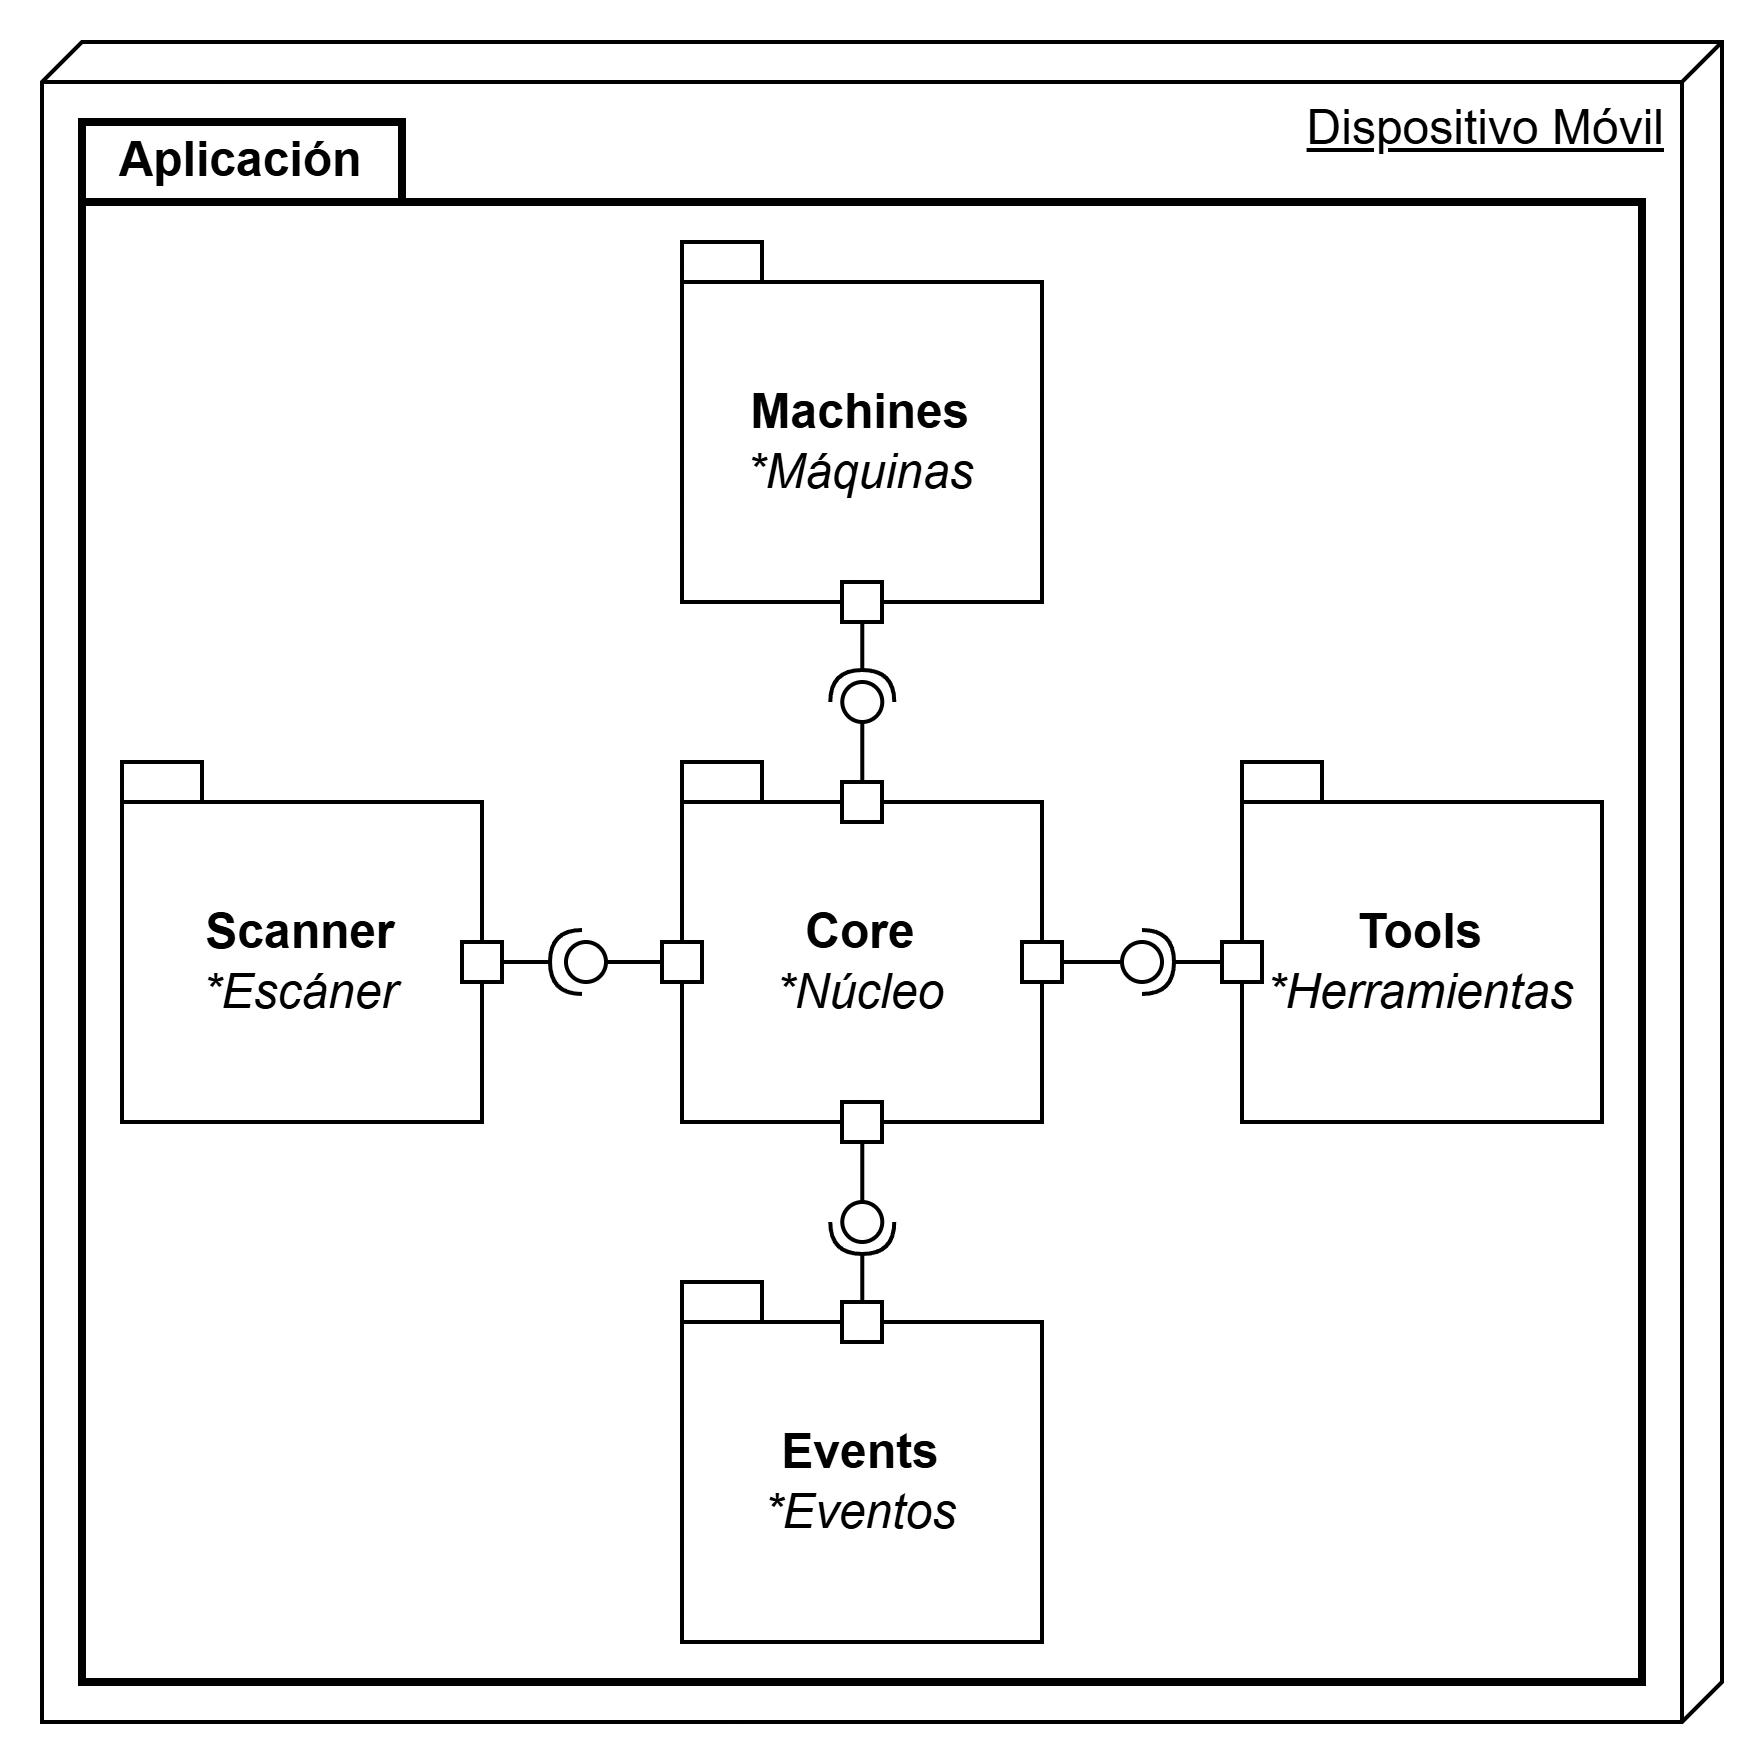
\includegraphics[width=0.8\textwidth]{assets/figures/second_phase/fig_uml_subsystems.png}
    \label{fig:subsystems}
    
\end{figure}
\fixvspace{0}

            \paragraph{Paquete de núcleo}

                Contiene la lógica y las definiciones transversales del aplicativo: el flujo de navegación entre pantallas, la declaración de la base de datos local, y los estilos compartidos entre subsistemas, incluyendo tipografías, colores, formas y utilidades comunes.

            \paragraph{Paquete de escáner}

                Agrupa la lógica y los componentes gráficos correspondientes a la sección de escáner, la cual implementa una previsualización de cámara en tiempo real para la lectura de marcadores, agilizando el acceso a la información de una máquina sin necesidad de realizar una navegación manual.

            \paragraph{Paquete de máquinas}

                Gestiona la lógica y los componentes gráficos de la sección de máquinas, abarcando la administración de información técnica, documentos PDF, marcadores, modelos 3D, lista de proveedores y actividades de mantenimiento con realidad aumentada.

            \paragraph{Paquete de herramientas}

                Agrupa la lógica y los componentes gráficos de la sección de herramientas, centralizando la disponibilidad de los instrumentos que pueden ser requeridos durante las actividades de mantenimiento vinculadas a las máquinas gestionadas en el subsistema de máquinas.

            \paragraph{Paquete de cronograma}

                Concentra la lógica y los componentes gráficos de la sección de cronograma, encargándose de la programación de eventos de mantenimiento y la gestión de notificaciones asociadas, donde dichos eventos corresponden a las actividades de mantenimiento vinculadas a las máquinas gestionadas en el subsistema de máquinas.

        \subsubsection{Flujo de navegación del aplicativo}

            La organización de los destinos del aplicativo se basa en un sistema de enrutamiento encargado de gestionar el flujo de navegación entre las diferentes secciones, controlando el acceso y la presentación de pantallas y componentes. Este sistema se representa mediante un árbol de navegación que define la jerarquía entre los destinos del aplicativo en la Figura \ref{fig:uml_navigation_state}.

            \begin{figure}[H]

    \caption{Secciones de navegación}
    \centering
    
    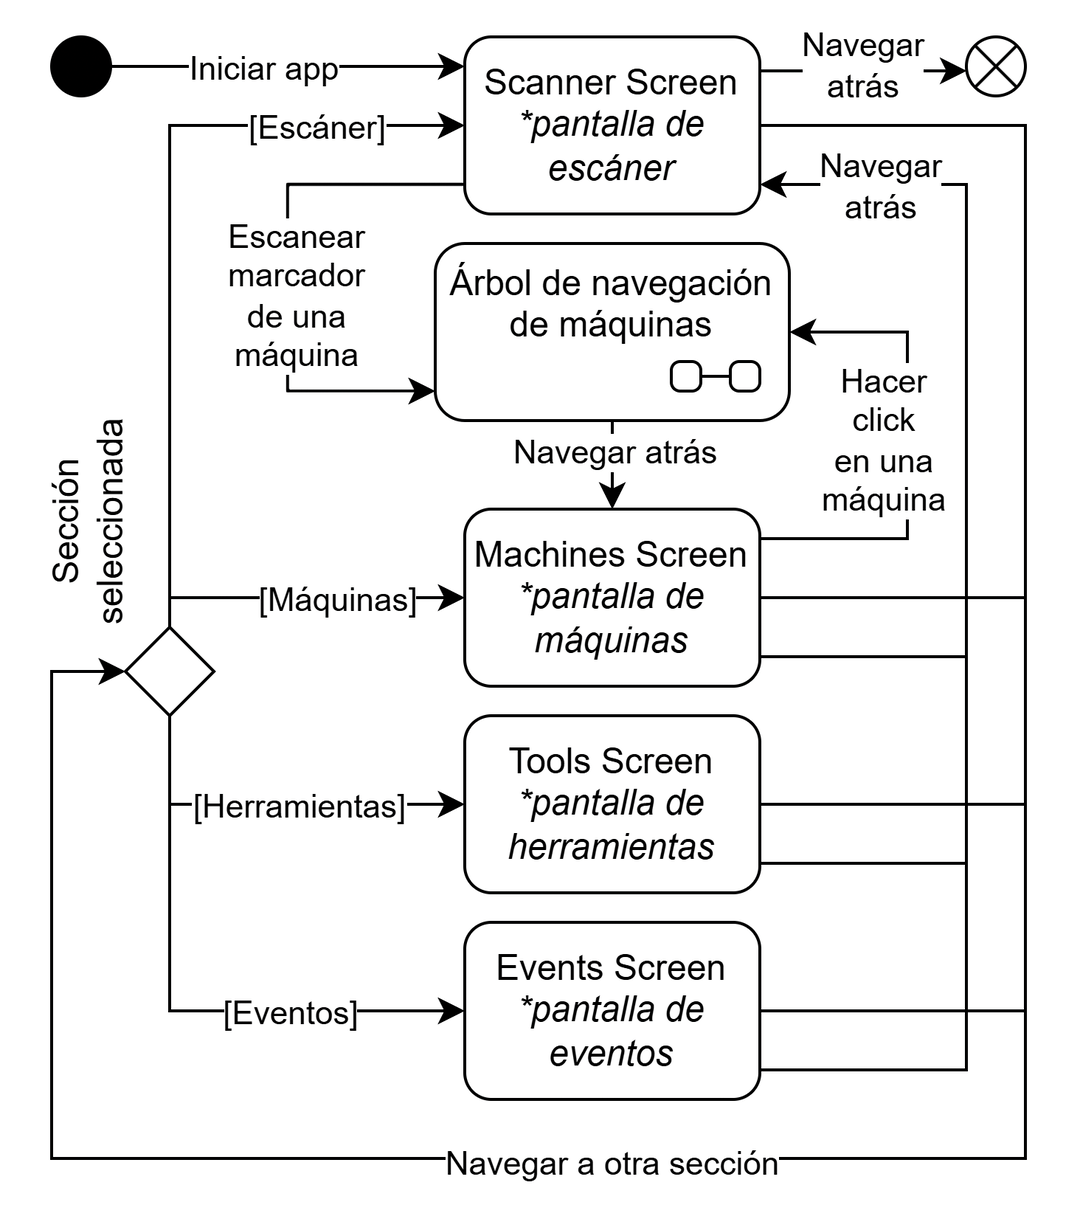
\includegraphics[width=1\textwidth]{assets/figures/second_phase/navigation/img_uml_navigation_state.png}
    \label{fig:uml_navigation_state}

\end{figure}
\fixvspace{1}

            \paragraph{Árboles de navegación anidados}

                A partir de la jerarquía principal, la sección de máquinas, al ser la única que cuenta con más de una pantalla, se define su propio árbol de navegación anidado, donde se administra de forma independiente su navegación interna, simplificando la comprensión del flujo principal (ver Figura \ref{fig:uml_navigation_machines_state}).

                \begin{figure}[H]

    \caption{Árbol de navegación anidado de máquinas}

    \centering
    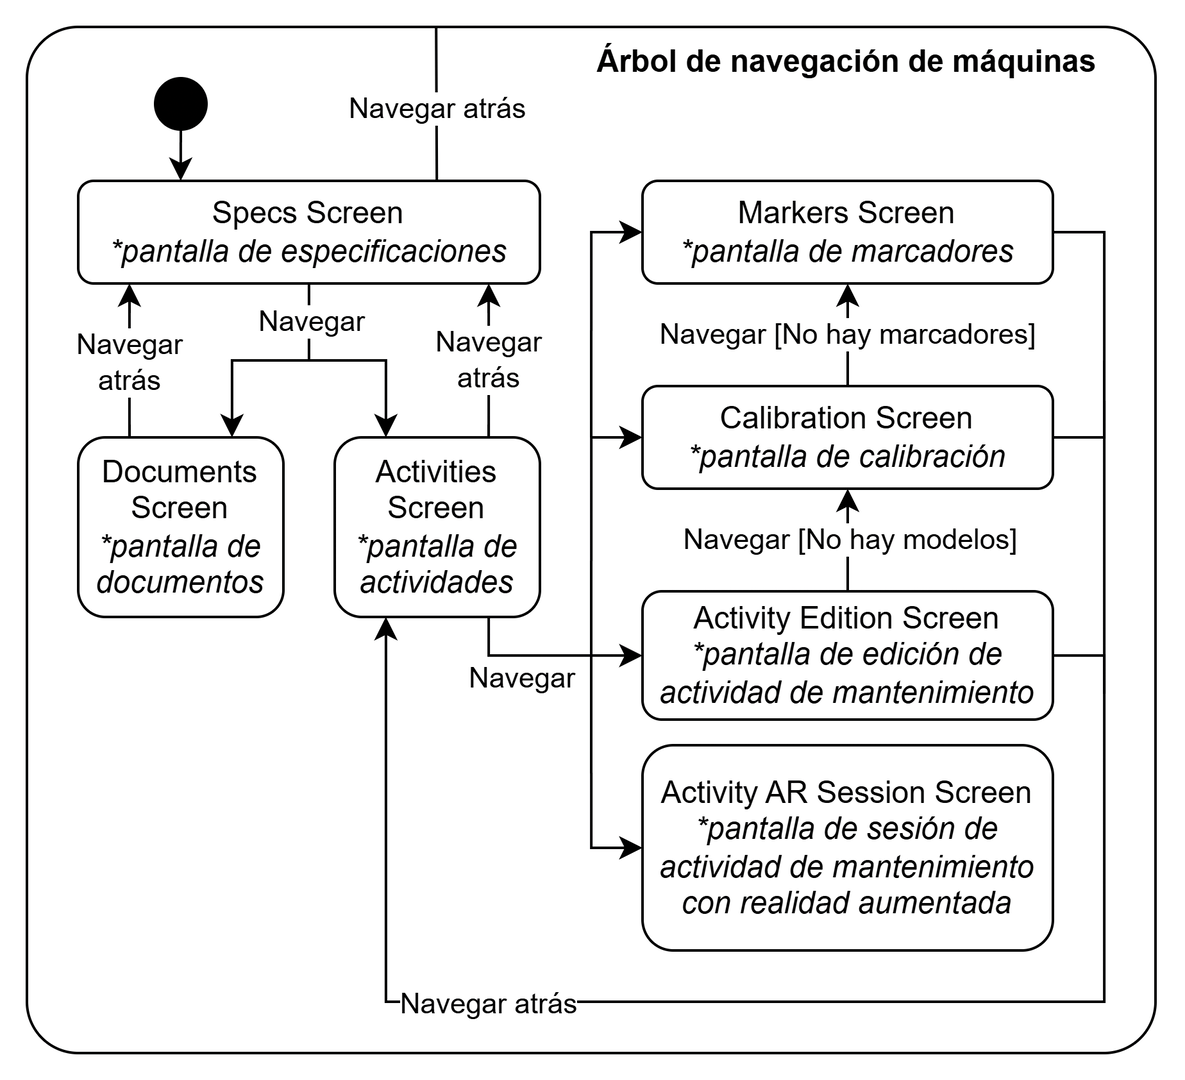
\includegraphics[width=1\textwidth]{assets/figures/second_phase/navigation/img_uml_navigation_machines_state.png}
    \label{fig:uml_navigation_machines_state}
    
\end{figure}
\fixvspace{1}
    
    \subsection{Arquitectura del sistema de bases de datos}

        El diseño de la base de datos se fundamenta en SQLite mediante el uso de la librería Room para Android, estructurándose en tablas de entidades simples y tablas de entidades compuestas según la naturaleza de los datos almacenados.

        \subsubsection{Tablas de entidades simples}

            Las tablas de entidades simples almacenan los datos individuales de un objeto en específico, agrupándose según su propósito funcional.

            \paragraph{Entidades de información técnica.}
            
                Almacenan los datos de identificación y especificaciones técnicas de la máquina y su motor eléctrico (ver Apéndices \ref{apc:entity_machine_and_specs} y \ref{apc:entity_motor_and_specs}). Cada equipo organiza su información en dos tablas: una destinada a la identidad y otro a las especificaciones técnicas, dado el volumen de atributos que cada una contiene. Adicionalmente, se incluye una entidad para los documentos PDF vinculados a cada máquina (ver Apéndice \ref{apc:entity_document}).

            \paragraph{Entidades de realidad aumentada.}
            
                Almacenan los datos de los elementos aumentados vinculados a cada máquina, los marcadores físicos que activan la experiencia de realidad aumentada y los modelos 3D superpuestos (ver Apéndice \ref{apc:entities_augmented_reality}). La entidad de marcador incluye un desplazamiento (offset) que define su posición relativa respecto a un nodo de origen. Dicho nodo actúa como referencia común para alinear los modelos dentro de una escena. De manera similar, la entidad de modelo también posee un desplazamiento relativo al nodo de origen.

            \paragraph{Entidades de procesos de mantenimiento.}
            
                Conforman una estructura secuencial que almacena la información sobre los procedimientos de mantenimiento asociados a cada máquina (ver Apéndice \ref{apc:entities_processes}).

            \paragraph{Entidades de catálogo.}
            
                Almacenan datos reutilizables de alcance global, sin vínculo directo a una máquina en particular. En este caso, corresponden al catálogo de herramientas disponibles durante las actividades de mantenimiento, cada una con representación visual vectorial según su tipo (ver Apéndice \ref{apc:entities_catalogue}).

            \paragraph{Entidad de cronograma.}
                
                Almacena los eventos de mantenimiento programados, cada uno vinculado a una actividad específica dentro del subsistema de máquinas. Gestiona tanto la recurrencia como la programación temporal de dichos eventos (ver Apéndice \ref{apc:entities_events}).

        \subsubsection{Tablas de entidades compuestas}

            Las tablas de entidades compuestas almacenan los registros de relaciones entre múltiples entidades, consolidando las llaves primarias (PK) de las entidades relacionadas para representar asociaciones de tipo muchos a muchos (N:N).

            \paragraph{Entidad de referencia para edición de modelos 3D en una operación.}
            
                Almacena la referencia de las partes de un modelo 3D asociadas a una operación de mantenimiento específica, actuando como tabla pivote entre la entidad de operación y la entidad de modelo (ver Apéndice \ref{apc:entity_edition}).

        \subsubsection{Modelo de relaciones}

            \paragraph{Relaciones de la entidad de máquinas.}
            
                La entidad de máquinas constituye el punto central del modelo relacional, la cual vincula entidades que almacenan datos técnicos, especificaciones y referencias a múltiples tareas. Estas relaciones se basan en llaves primarias (PK) y llaves foráneas (FK), siendo comúnmente de tipo uno a uno (1:1) o uno a muchos (1:N), como se muestra en la Figura \ref{fig:relation_machine_entities}.

                \begin{figure}[H]
    \caption{Relaciones generales de una máquina}
    \centering
    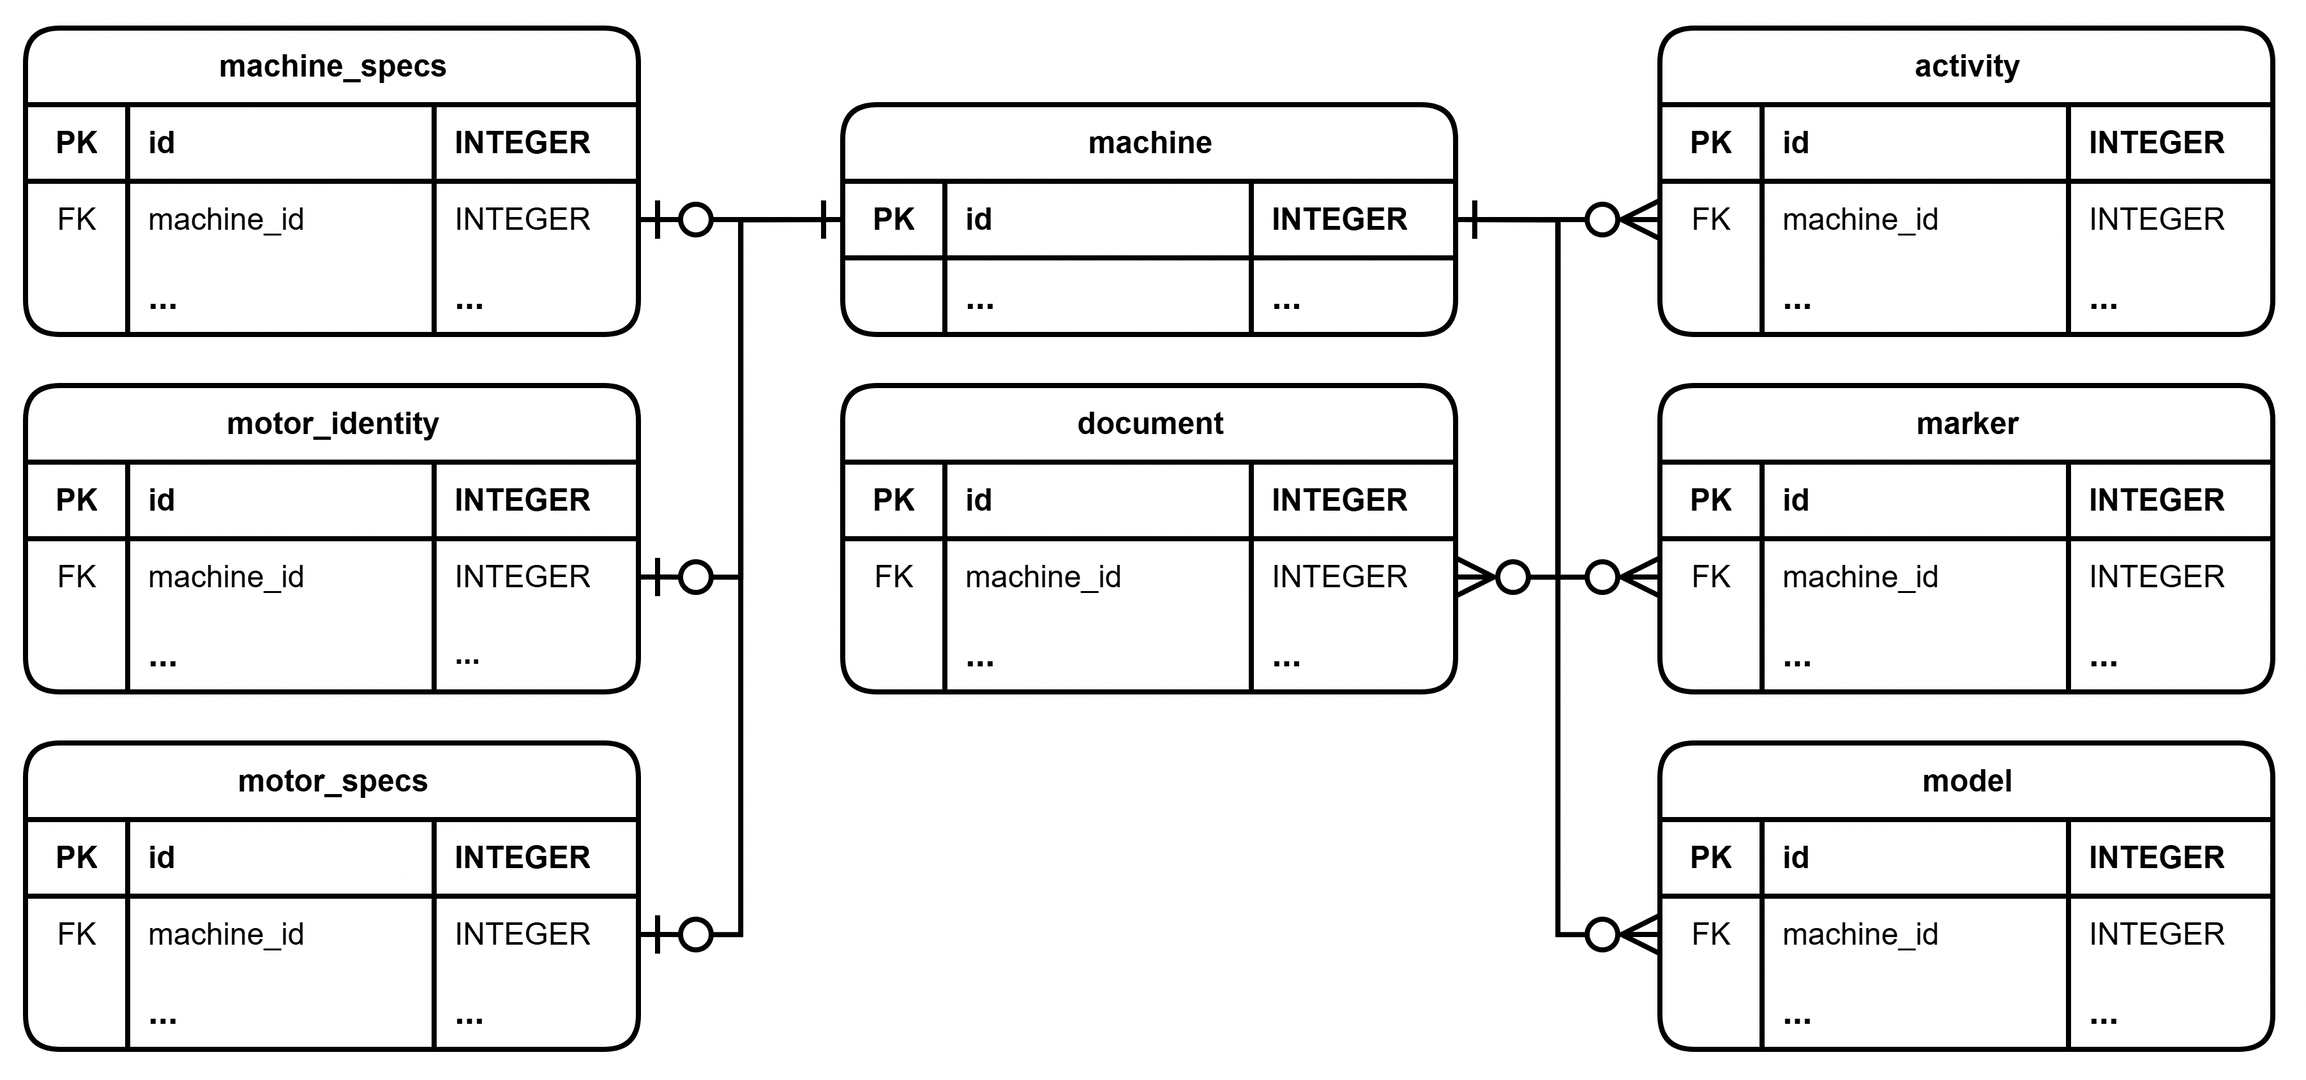
\includegraphics[width=\textwidth]{assets/figures/second_phase/relation/img_relations_machine_entities.png}
    \label{fig:relation_machine_entities}
\end{figure}
\fixvspace{1}

            \paragraph{Relaciones de la cadena jerárquica de mantenimiento.}
            
                %AGREGAR QUE ES UNA ACTIVIDAD

                Para el mantenimiento de una máquina se conforma una cadena jerárquica que estructura los procedimientos: una actividad agrupa una serie de pasos ordenados que contiene un título, descripción y una imagen ilustrativa, mientras que cada paso contiene varias operaciones, las cuales definen las animaciones 3D ejecutadas sobre las partes individuales de un modelo durante la experiencia de realidad aumentada, como se muestra en la Figura \ref{fig:relation_activity_entities}.

                \begin{figure}[H]
    \caption{Relaciones para un proceso de mantenimiento}
    \centering
    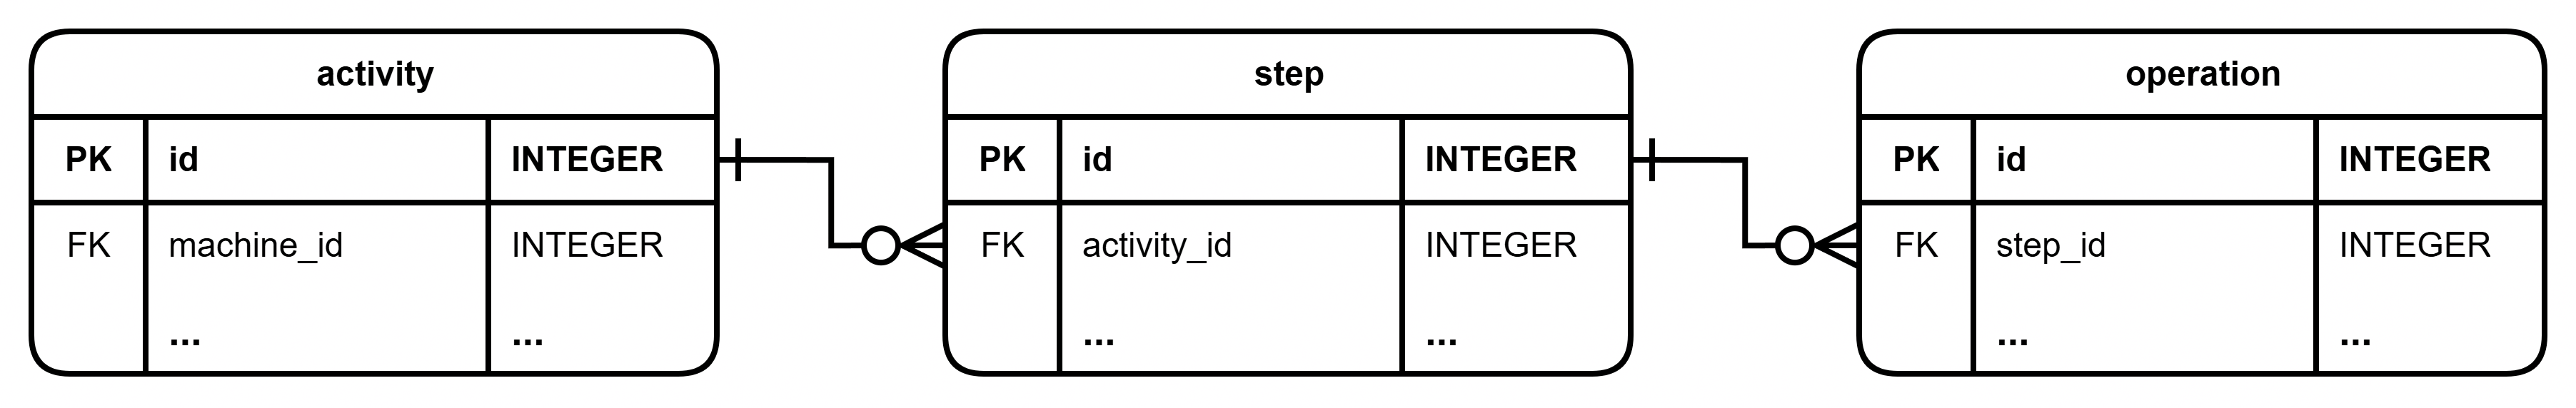
\includegraphics[width=\textwidth]{assets/figures/second_phase/relation/img_relations_activity_entities.png}
    \label{fig:relation_activity_entities}
\end{figure}
\fixvspace{1}

            \paragraph{Relación pivote entre operaciones y modelos 3D.}
                
                La edición de un proceso de mantenimiento requiere almacenar de forma independiente la referencia de cada subparte o submodelo de un modelo 3D, entendidas como las partes individuales sobre las cuales se aplica la animación definida por una operación. Para ello, se emplea una entidad pivote que se relaciona de forma muchos a muchos (N:N) entre la entidad de operación y la entidad de modelo, como se muestra en la Figura \ref{fig:relation_pivot_entities}.

                \begin{figure}[H]
    \caption{Relaciones de entidades de edición de procesos de mantenimiento}
    \centering
    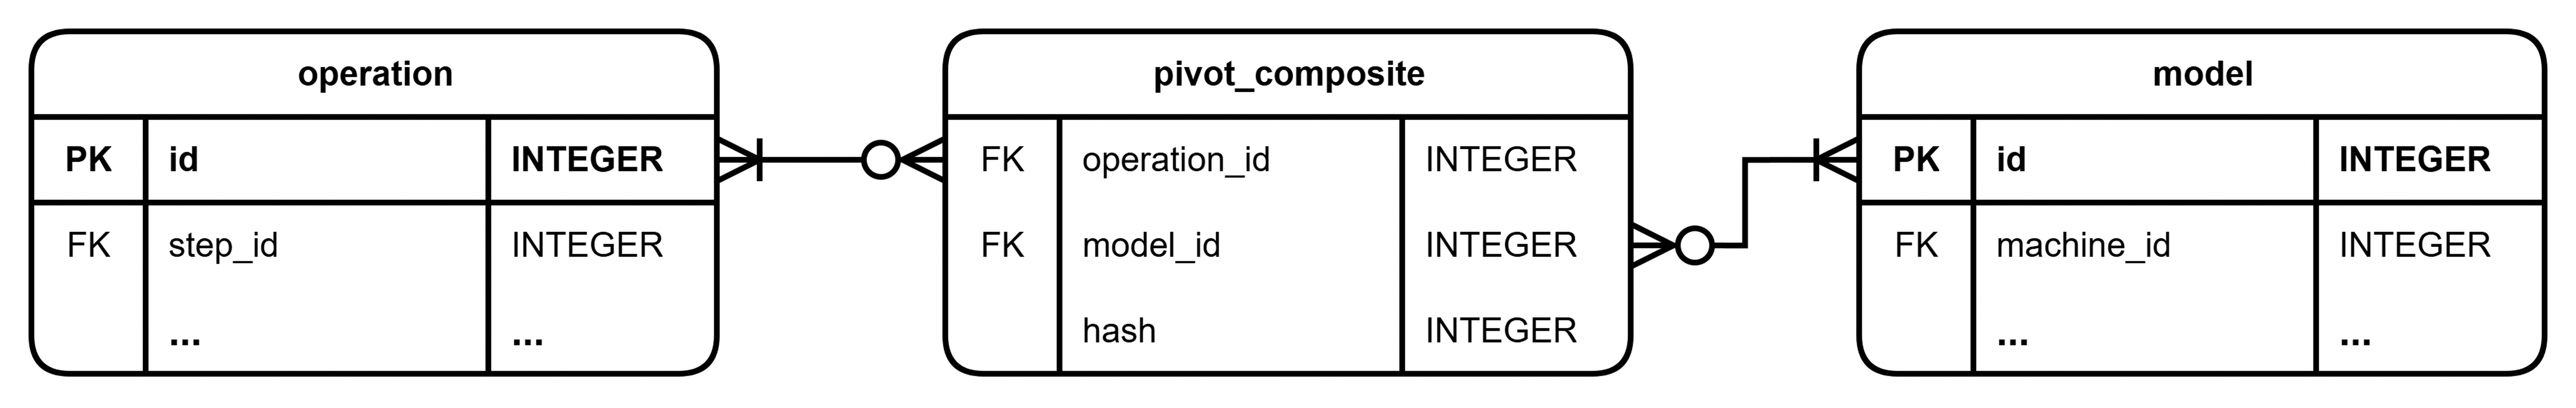
\includegraphics[width=\textwidth]{assets/figures/second_phase/relation/img_relations_pivot_entities.png}
    \label{fig:relation_pivot_entities}
\end{figure}
\fixvspace{1}

    \subsection{Herramientas de modelado paramétrico}

        Para la construcción del modelo de prueba y sus componentes mecánicos, se utilizaron herramientas CAD (diseño asistido por computadora), específicamente OnShape y SolidWorks. Estas herramientas permitieron realizar el modelado paramétrico de las piezas, así como el ensamblaje de componentes, necesario para la posterior generación de animaciones aplicadas en la experiencia de realidad aumentada.
    
    \subsection{Herramientas de exportación en glTF}

        Para la exportación de los modelos tridimensionales se utilizó Blender como herramienta de procesamiento y generación de archivos en formato .glb bajo el estándar glTF. Su uso permitió mantener la unicidad en los nombres de cada pieza o submodelo durante el proceso de exportación, característica necesaria para la generación de identificadores hash asociados a las partes individuales de cada modelo 3D.

    \subsection{Recursos externos}

        \subsubsection{Formatos de los archivos}

            Para garantizar la compatibilidad con las herramientas utilizadas y con el motor de renderizado de la aplicación, se usó el formato de transmisión de biblioteca de gráficos (.glTF) en su versión binaria (.glb), mientras que los formatos compatibles de imágenes fueron: .png, .jpeg, .jpg, .tiff y .webp.

    \subsection{Escena de realidad aumentada}

        La escena de realidad aumentada fue implementada mediante la librería SceneView para Android, la cual integra el motor de renderizado Filament junto con el kit de desarrollo ARCore de Google. Esta combinación permitió administrar el renderizado de modelos tridimensionales, el seguimiento espacial del dispositivo y el posicionamiento dinámico de contenido virtual durante las sesiones de realidad aumentada.

        De acuerdo con \textcite{GOOGLE:2025}, ARCore proporciona tres capacidades principales utilizadas durante la implementación de la escena:

        \begin{enumerate}

            \item \textbf{Seguimiento de movimiento:} permite identificar y rastrear puntos característicos del entorno, estimando la posición y orientación del dispositivo en tiempo real, mediante visión computacional y sensores inerciales. 
            
            \item \textbf{Comprensión del entorno:} permite la detección de superficies horizontales, verticales e inclinadas.

            \item \textbf{Estimación de luz:} permite aproximar las condiciones de iluminación del entorno para mejorar la integración visual de modelos renderizados.

        \end{enumerate}

        \subsubsection{Sistema de coordenadas de la escena}

            Durante la implementación de la escena de realidad aumentada fue necesario trabajar con el sistema de coordenadas utilizado por ARCore y los dispositivos Android para garantizar el posicionamiento correcto de los modelos tridimensionales. Este sistema corresponde a un esquema de coordenadas de mano derecha definido respecto a la orientación natural de la pantalla del dispositivo (ver Figura \ref{fig:coordinate_system_devices}).

            Dentro de este sistema, el eje X se extiende horizontalmente hacia la derecha de la pantalla, el eje Y verticalmente hacia arriba y el eje Z perpendicular al plano de la pantalla en dirección al usuario.

            \begin{figure}[H]
    \caption{Sistema de coordenadas de dispositivos}
    \centering
    \setlength{\tabcolsep}{0pt}
    \renewcommand{\arraystretch}{1.2}
    \begin{tabular}{
        |>{\centering\arraybackslash}m{(\textwidth - 3\arrayrulewidth) / 2}
        |>{\centering\arraybackslash}m{(\textwidth - 3\arrayrulewidth) / 2}|
    }
        \hline

        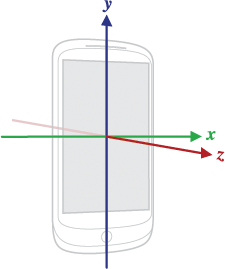
\includegraphics[width=0.4\textwidth]
        {assets/figures/second_phase/coordinate_system/img_coordinate_system_portrait.png} &
            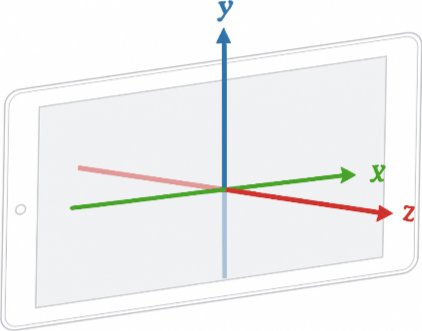
\includegraphics[width=0.4\textwidth]
        {assets/figures/second_phase/coordinate_system/img_coordinate_system_landscape.png} \\

        \small Dispositivo con orientación natural en modo retrato &
            \small Dispositivo con orientación natural en modo paisaje \\
        
        \hline
    \end{tabular}
    \caption*{\textit{Nota}. \textnormal{Imagen de modo retrato extraída de: \url{https://developer.android.com/develop/sensors-and-location/sensors/sensors_overview\#sensors-coords}}}
    \label{fig:coordinate_system_devices}
\end{figure}
\fixvspace{0.5}
            
            Durante las pruebas de posicionamiento se observó que la orientación física del dispositivo no altera la definición de los ejes del sistema de coordenadas. Esto permitió mantener la alineación vertical de los modelos respecto al suelo al iniciar sesiones de realidad aumentada, independientemente de la dirección hacia la cual estuviera orientada la cámara, como se muestra en la Figura \ref{fig:coordinate_system_scene}.

            \begin{figure}[H]
    \caption{Sistema de coordenadas de la escena de realidad aumentada}
    \centering
    \borderedgraphics{assets/figures/second_phase/coordinate_system/img_coordinate_system_scene.png}
    \label{fig:coordinate_system_scene}
\end{figure}
\fixvspace{1}

    \subsection{Nodos de la escena}

        La escena de realidad aumentada fue implementada mediante una arquitectura jerárquica de nodos encargada de administrar transformaciones espaciales, renderizado y manipulación de modelos tridimensionales. Esta estructura combinó nodos proporcionados por SceneView y ARCore junto a nodos personalizados, los cuales fueron desarrollados para resolver limitaciones de posicionamiento, selección y edición de submodelos dentro de la escena.

        \subsubsection{Sistema de coordenadas de los nodos}

            El sistema de coordenadas global corresponde al sistema principal de la escena de realidad aumentada. En contraste, cada nodo mantiene un sistema de coordenadas local definido respecto a su nodo padre, permitiendo aplicar transformaciones relativas dentro de la jerarquía de nodos sin alterar la estructura general de la escena.

            Esta organización permitió conservar relaciones espaciales entre modelos y submodelos facilitando el posicionamiento de elementos dentro de la escena. La relación entre los sistemas de coordenadas globales y locales se muestra en la Figura \ref{fig:coordinate_system_comparison}.

            \begin{figure}[H]

    \caption{Comparación de los sistemas de coordenadas relativos contra el global de la escena en su esquina inferior izquierda}

    \centering
    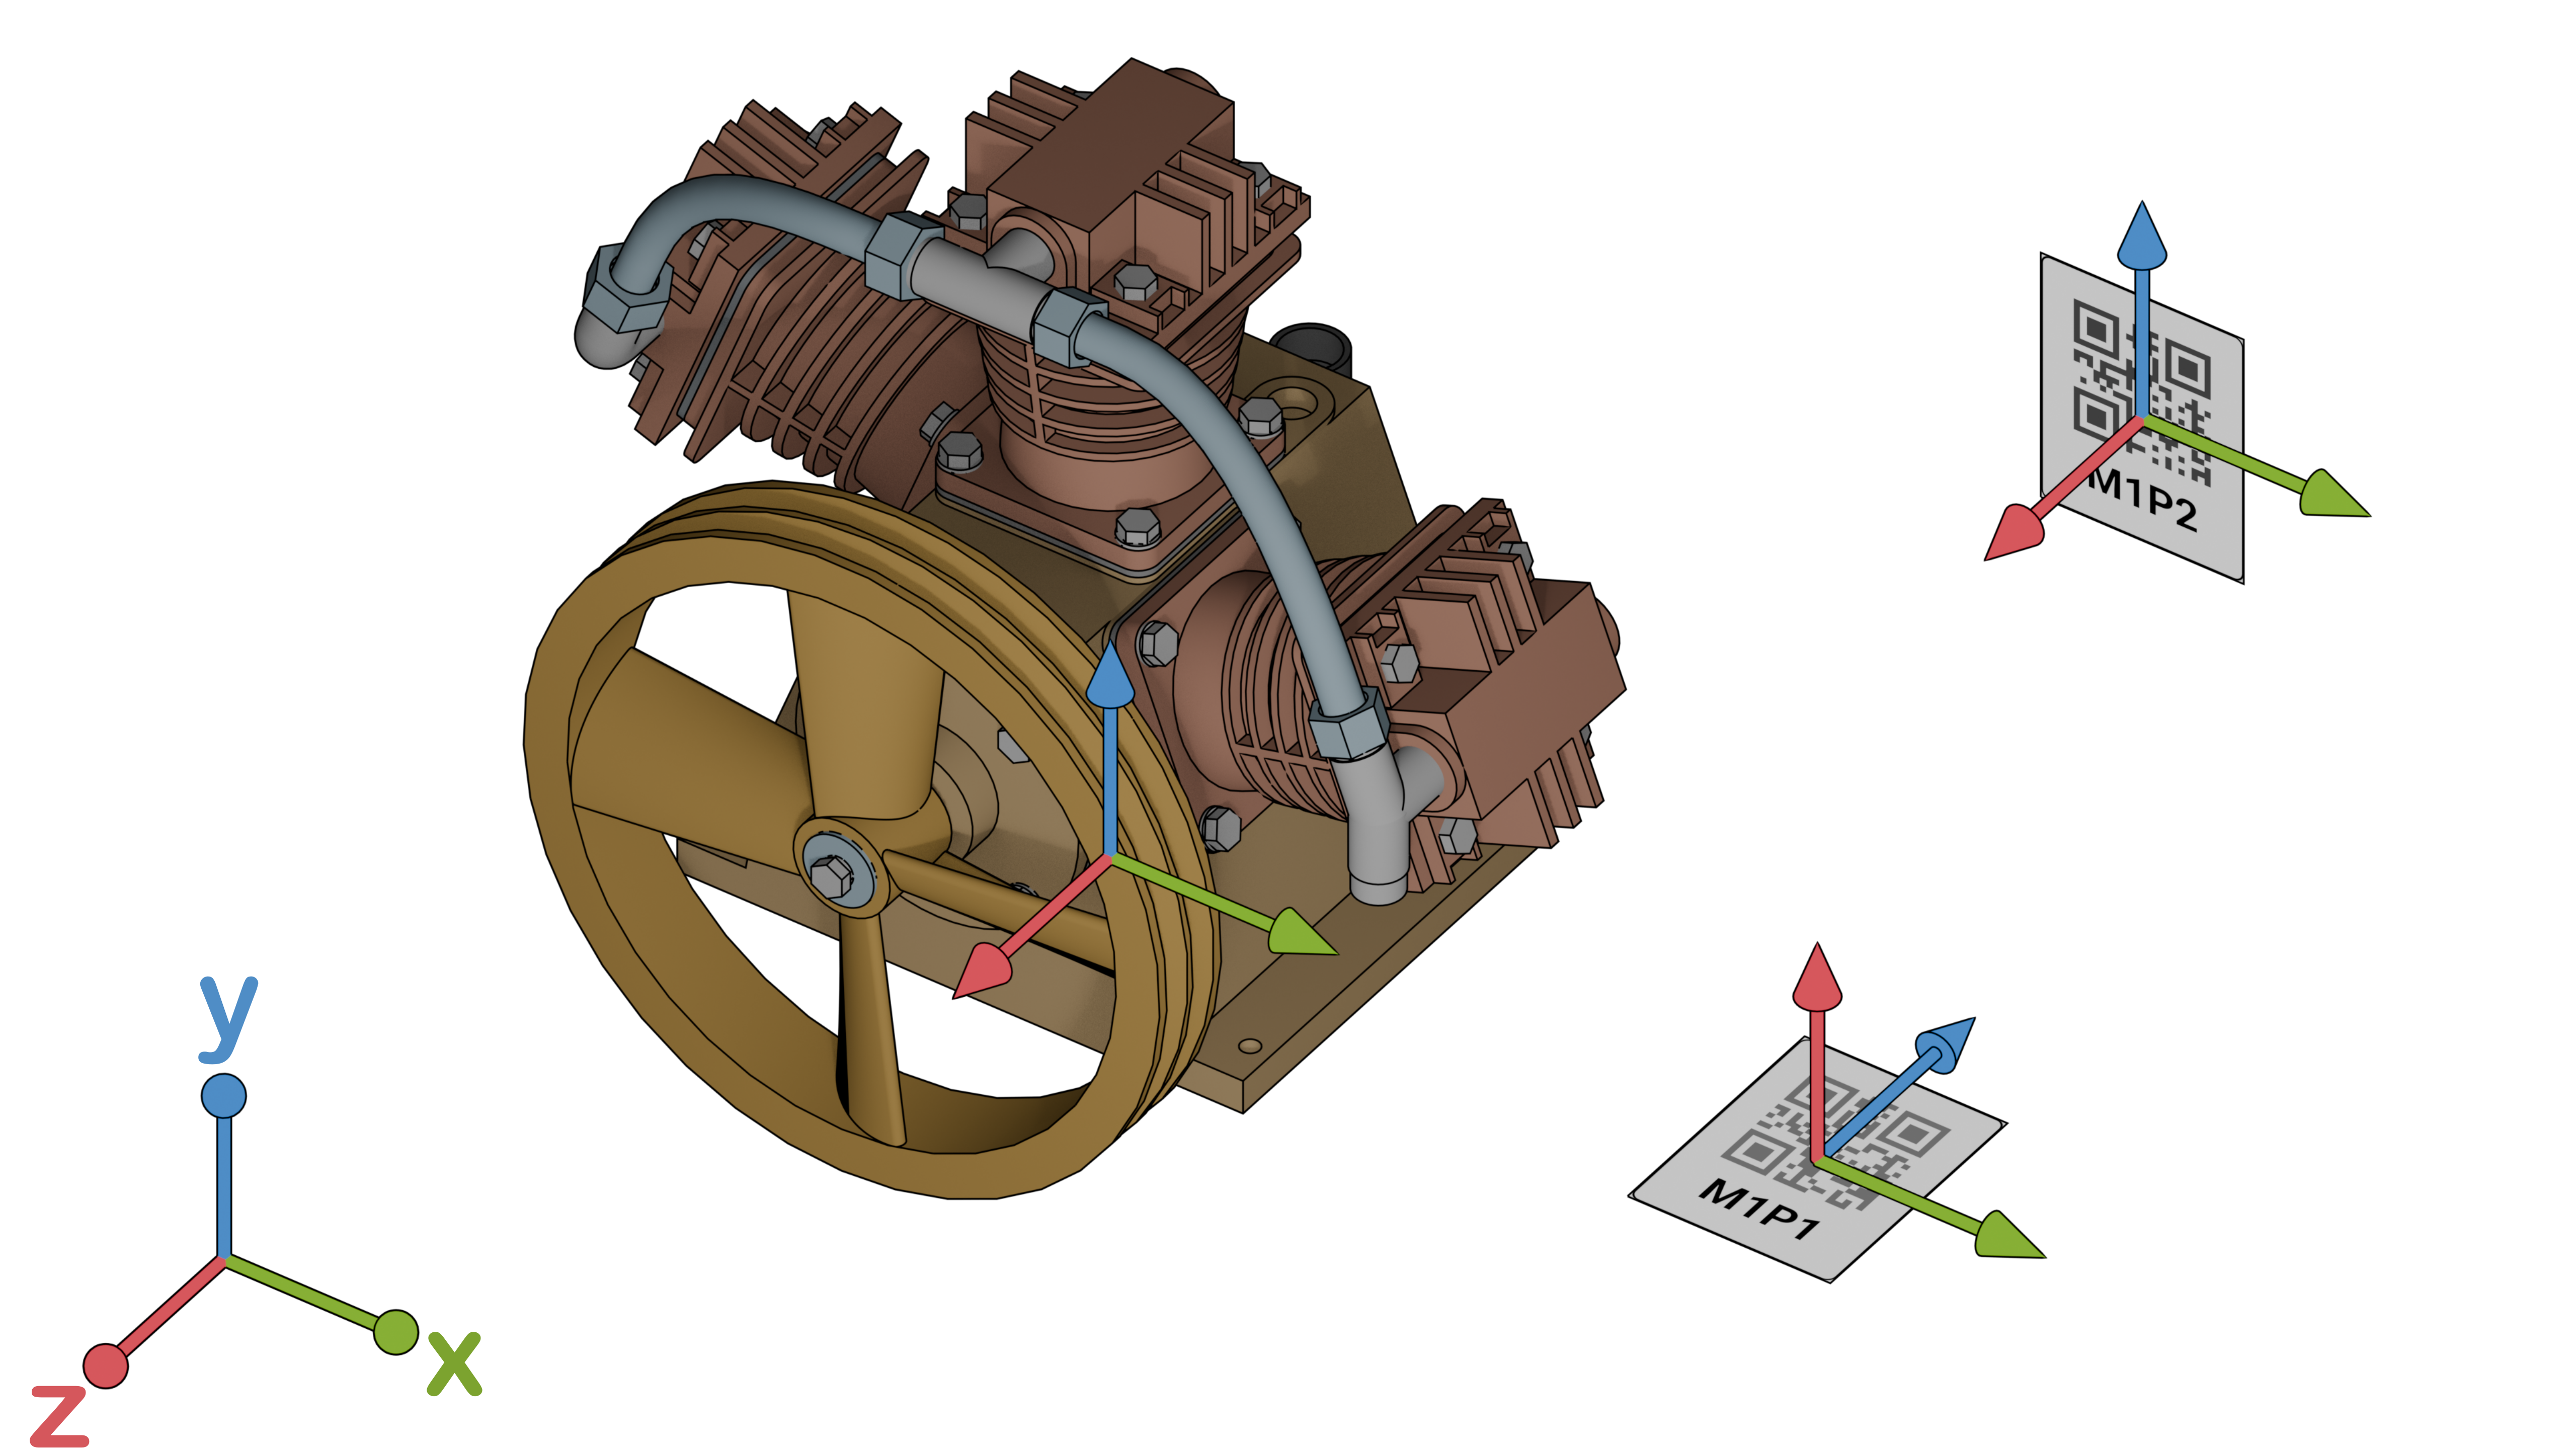
\includegraphics[width=1.0\textwidth]{assets/figures/second_phase/coordinate_system/img_coordinate_system_comparison.png}
    \label{fig:coordinate_system_comparison}
    
\end{figure}
\vspace{-1.6\baselineskip}

        \subsubsection{Clase base de los nodos}

            Para la implementación de la jerarquía de nodos se utilizó inicialmente una clase base encargada de proporcionar propiedades comunes de transformación, interacción y renderizado. A partir de esta estructura se desarrollaron nodos especializados orientados al seguimiento espacial, manipulación de modelos y asistencia visual dentro de la escena de realidad aumentada, como puede observarse en el diagrama de la Figura \ref{fig:uml_node_inheritance}.

            \begin{figure}[H]
    \caption{Herencia de la clase base}
    \centering
    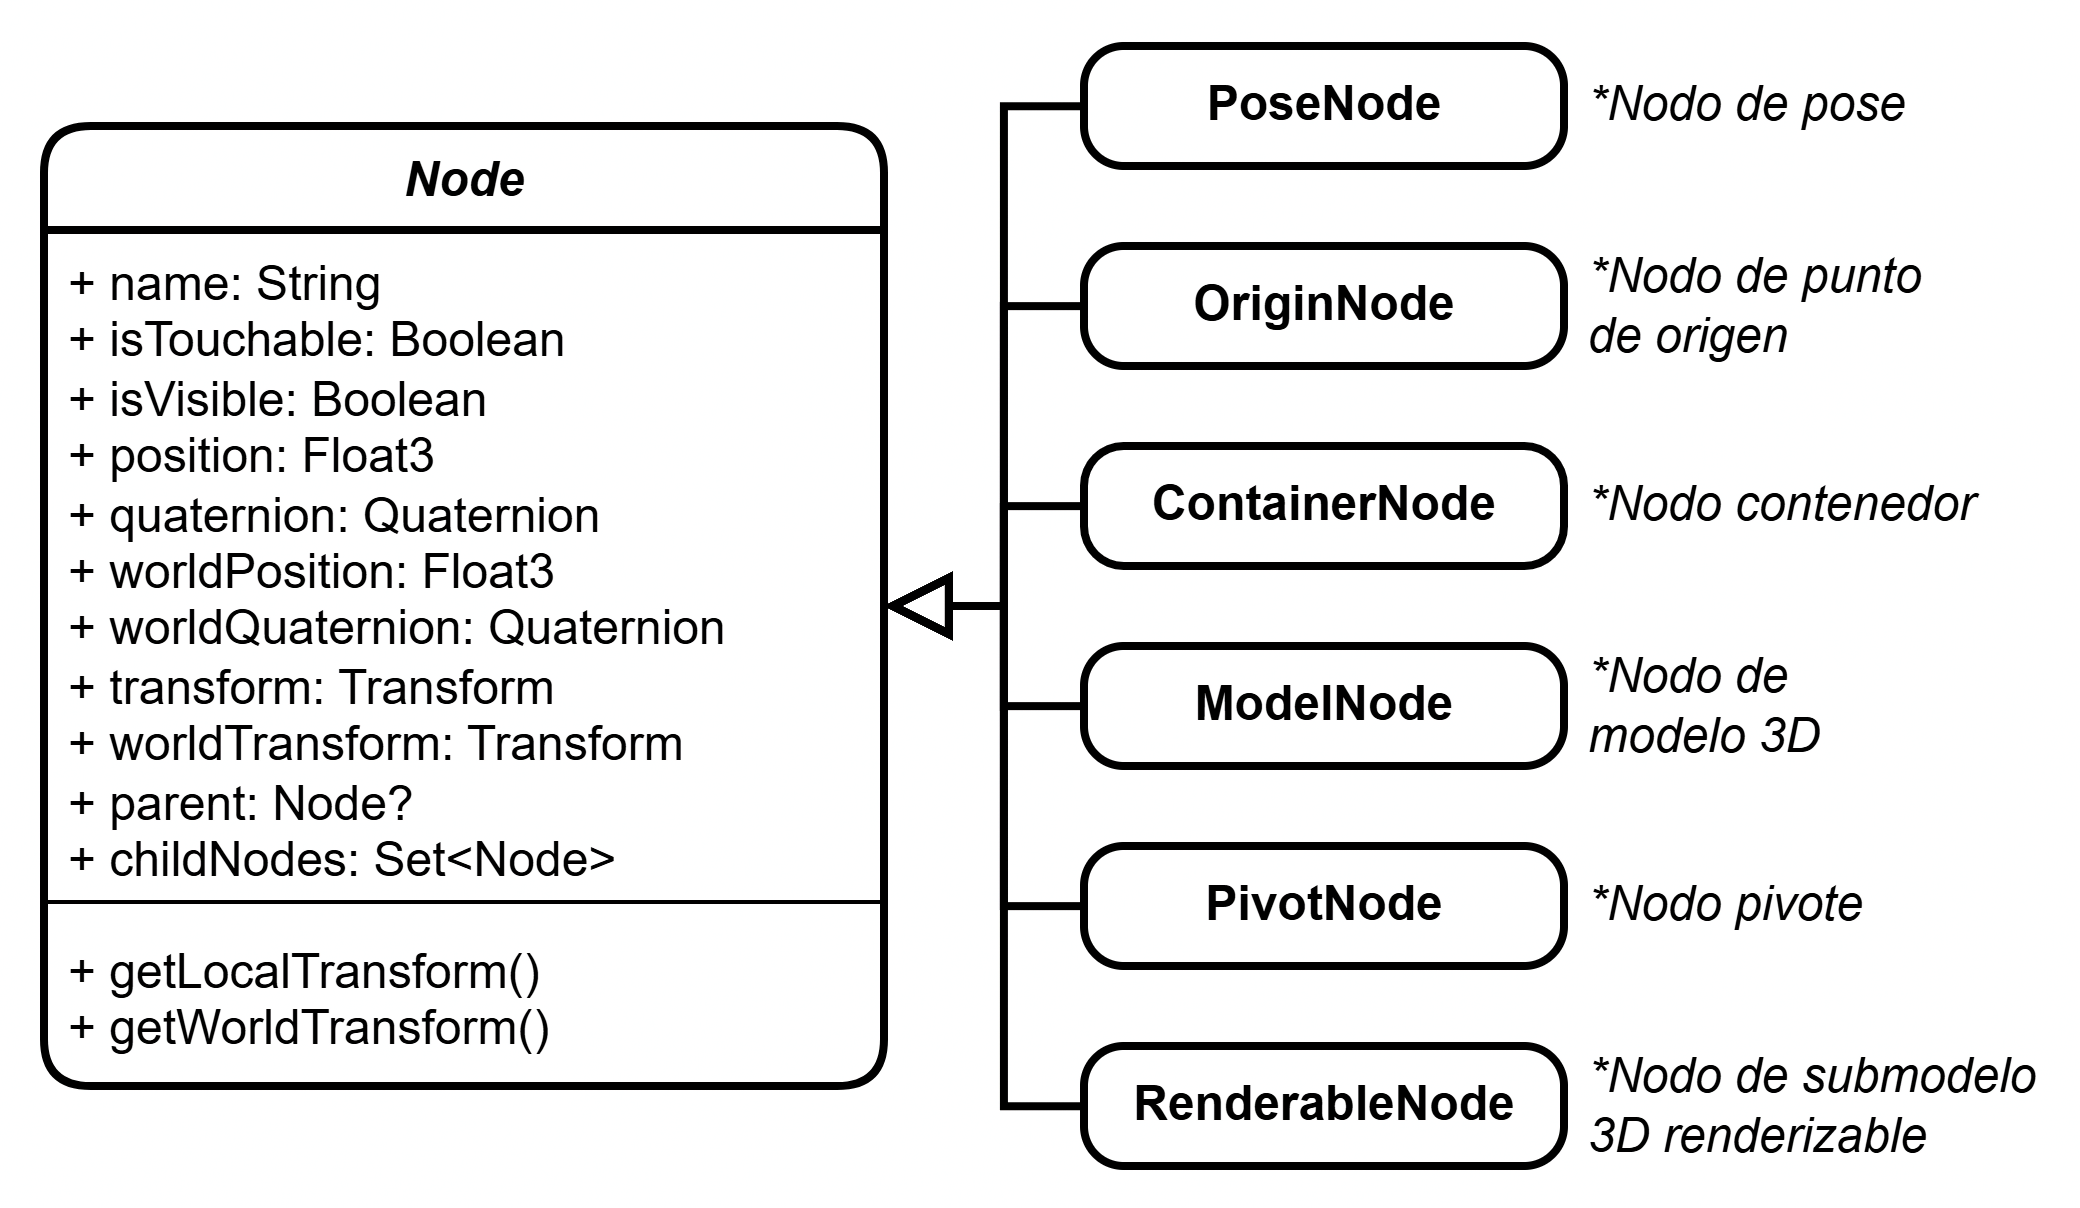
\includegraphics[width=0.8\textwidth]{assets/figures/second_phase/diagram/img_uml_node_inheritance.png}
    \label{fig:uml_node_inheritance}
\end{figure}
\fixvspace{0}

        \subsubsection{Nodos de asistencia visual}

            Como parte de la interacción con los modelos tridimensionales, se implementaron nodos geométricos auxiliares utilizados para la representación visual de herramientas de edición y asistencia espacial. Estos nodos permitieron desarrollar elementos interactivos como ejes, cajas de selección, controles de transformación visual y marcadores visuales, como se muestra en la Figura \ref{fig:uml_geometry_inheritance}.

            \begin{figure}[H]

    \caption{Nodos de asistencia visual y sus composiciones}

    \centering
    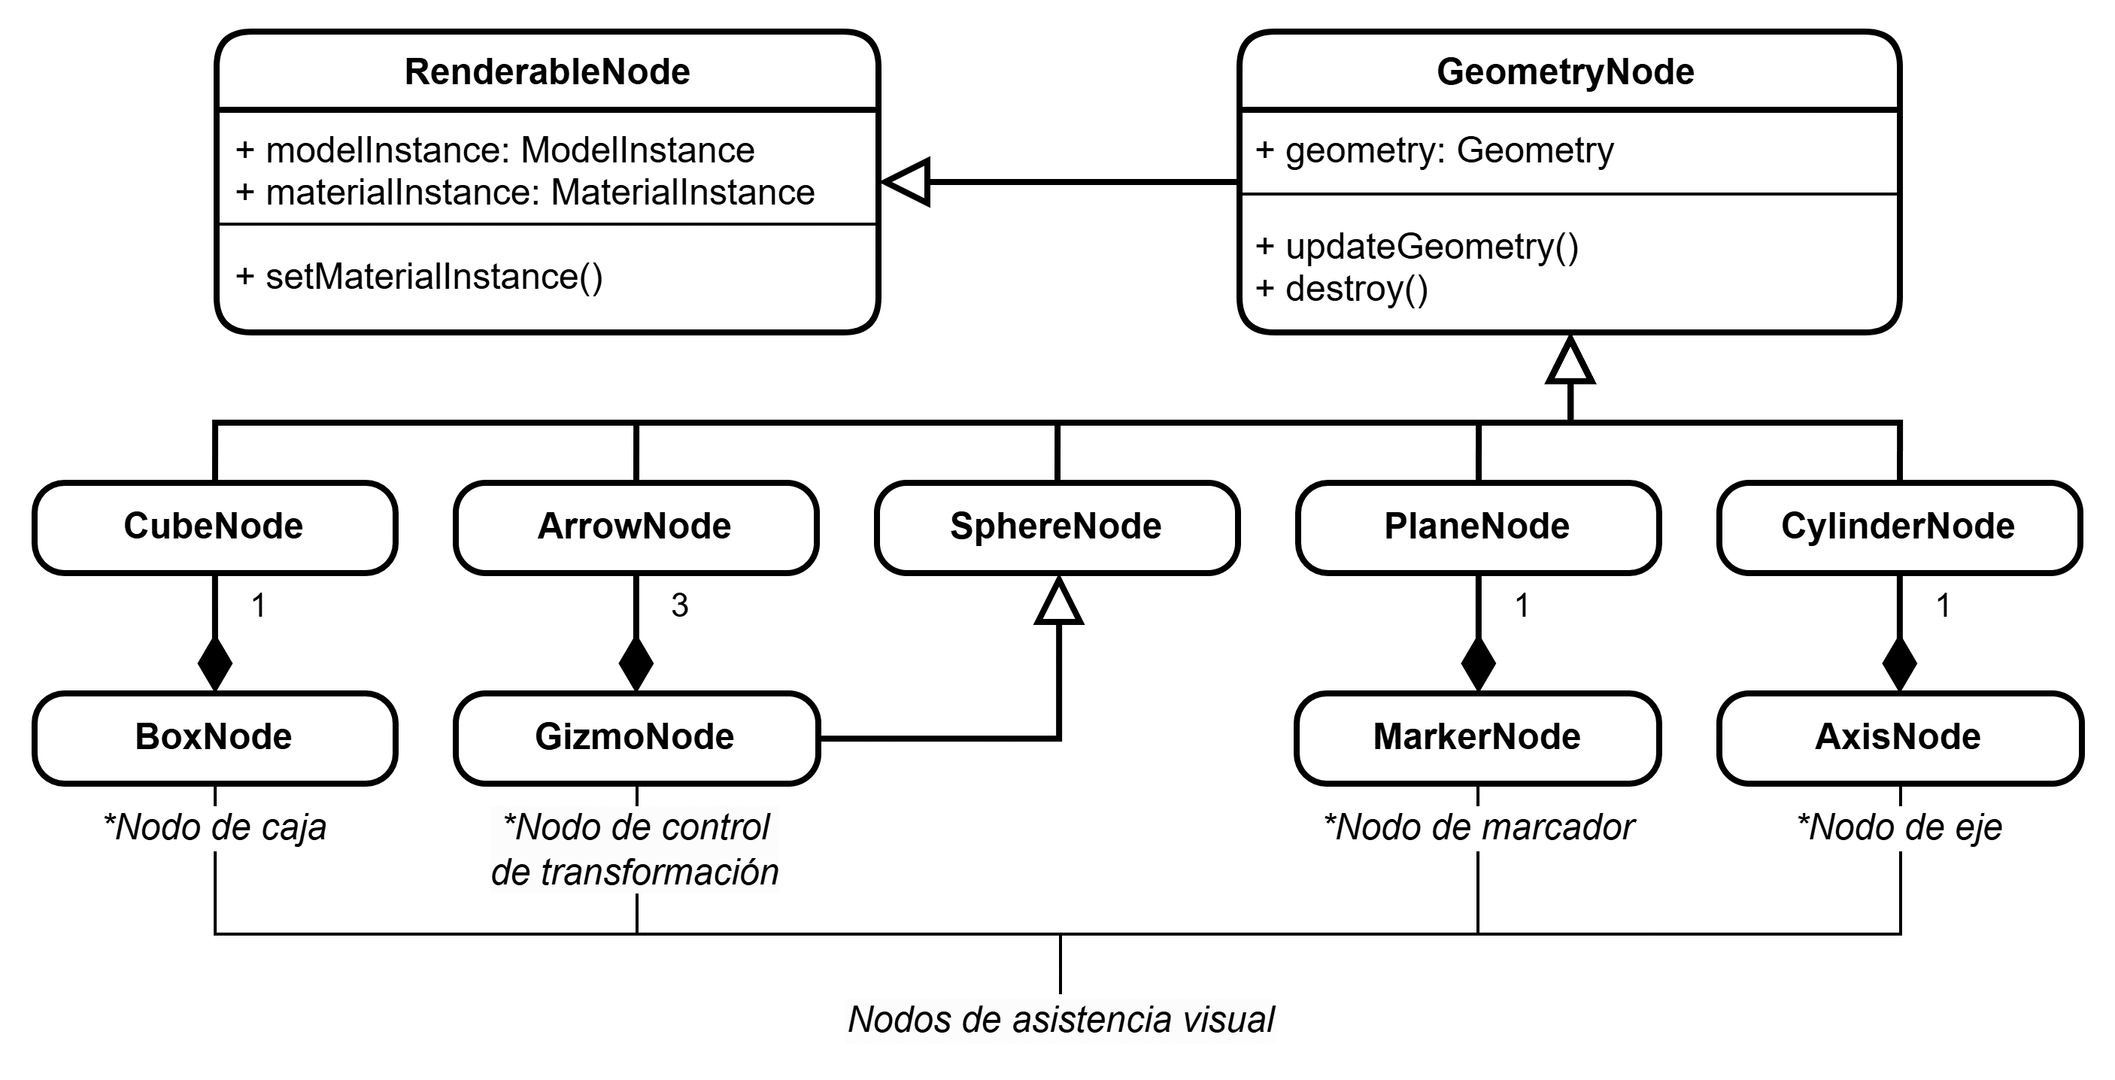
\includegraphics[width=1\textwidth]{assets/figures/second_phase/diagram/img_uml_geometry_inheritance.png}
    \label{fig:uml_geometry_inheritance}
    
\end{figure}
\fixvspace{1}

            \paragraph{Nodos geométricos}
            
                Representaron la base para la construcción de los nodos de asistencia visual dentro de la escena de realidad aumentada. Están compuestos por un conjunto de mallas (\textit{meshes}) formadas mediante primitivas geométricas como puntos, líneas y triángulos. Cada primitiva almacena información propia de geometría, incluyendo vértices, normales, coordenadas UV y materiales asociados. Estos se tratan de figuras tridimensionales simples como cubos, flechas, esferas, planos y cilindros, como se muestra en la Figura \ref{fig:node_geometry}.

                \begin{figure}[H]

    \caption{Nodo de geometría}

    \centering
    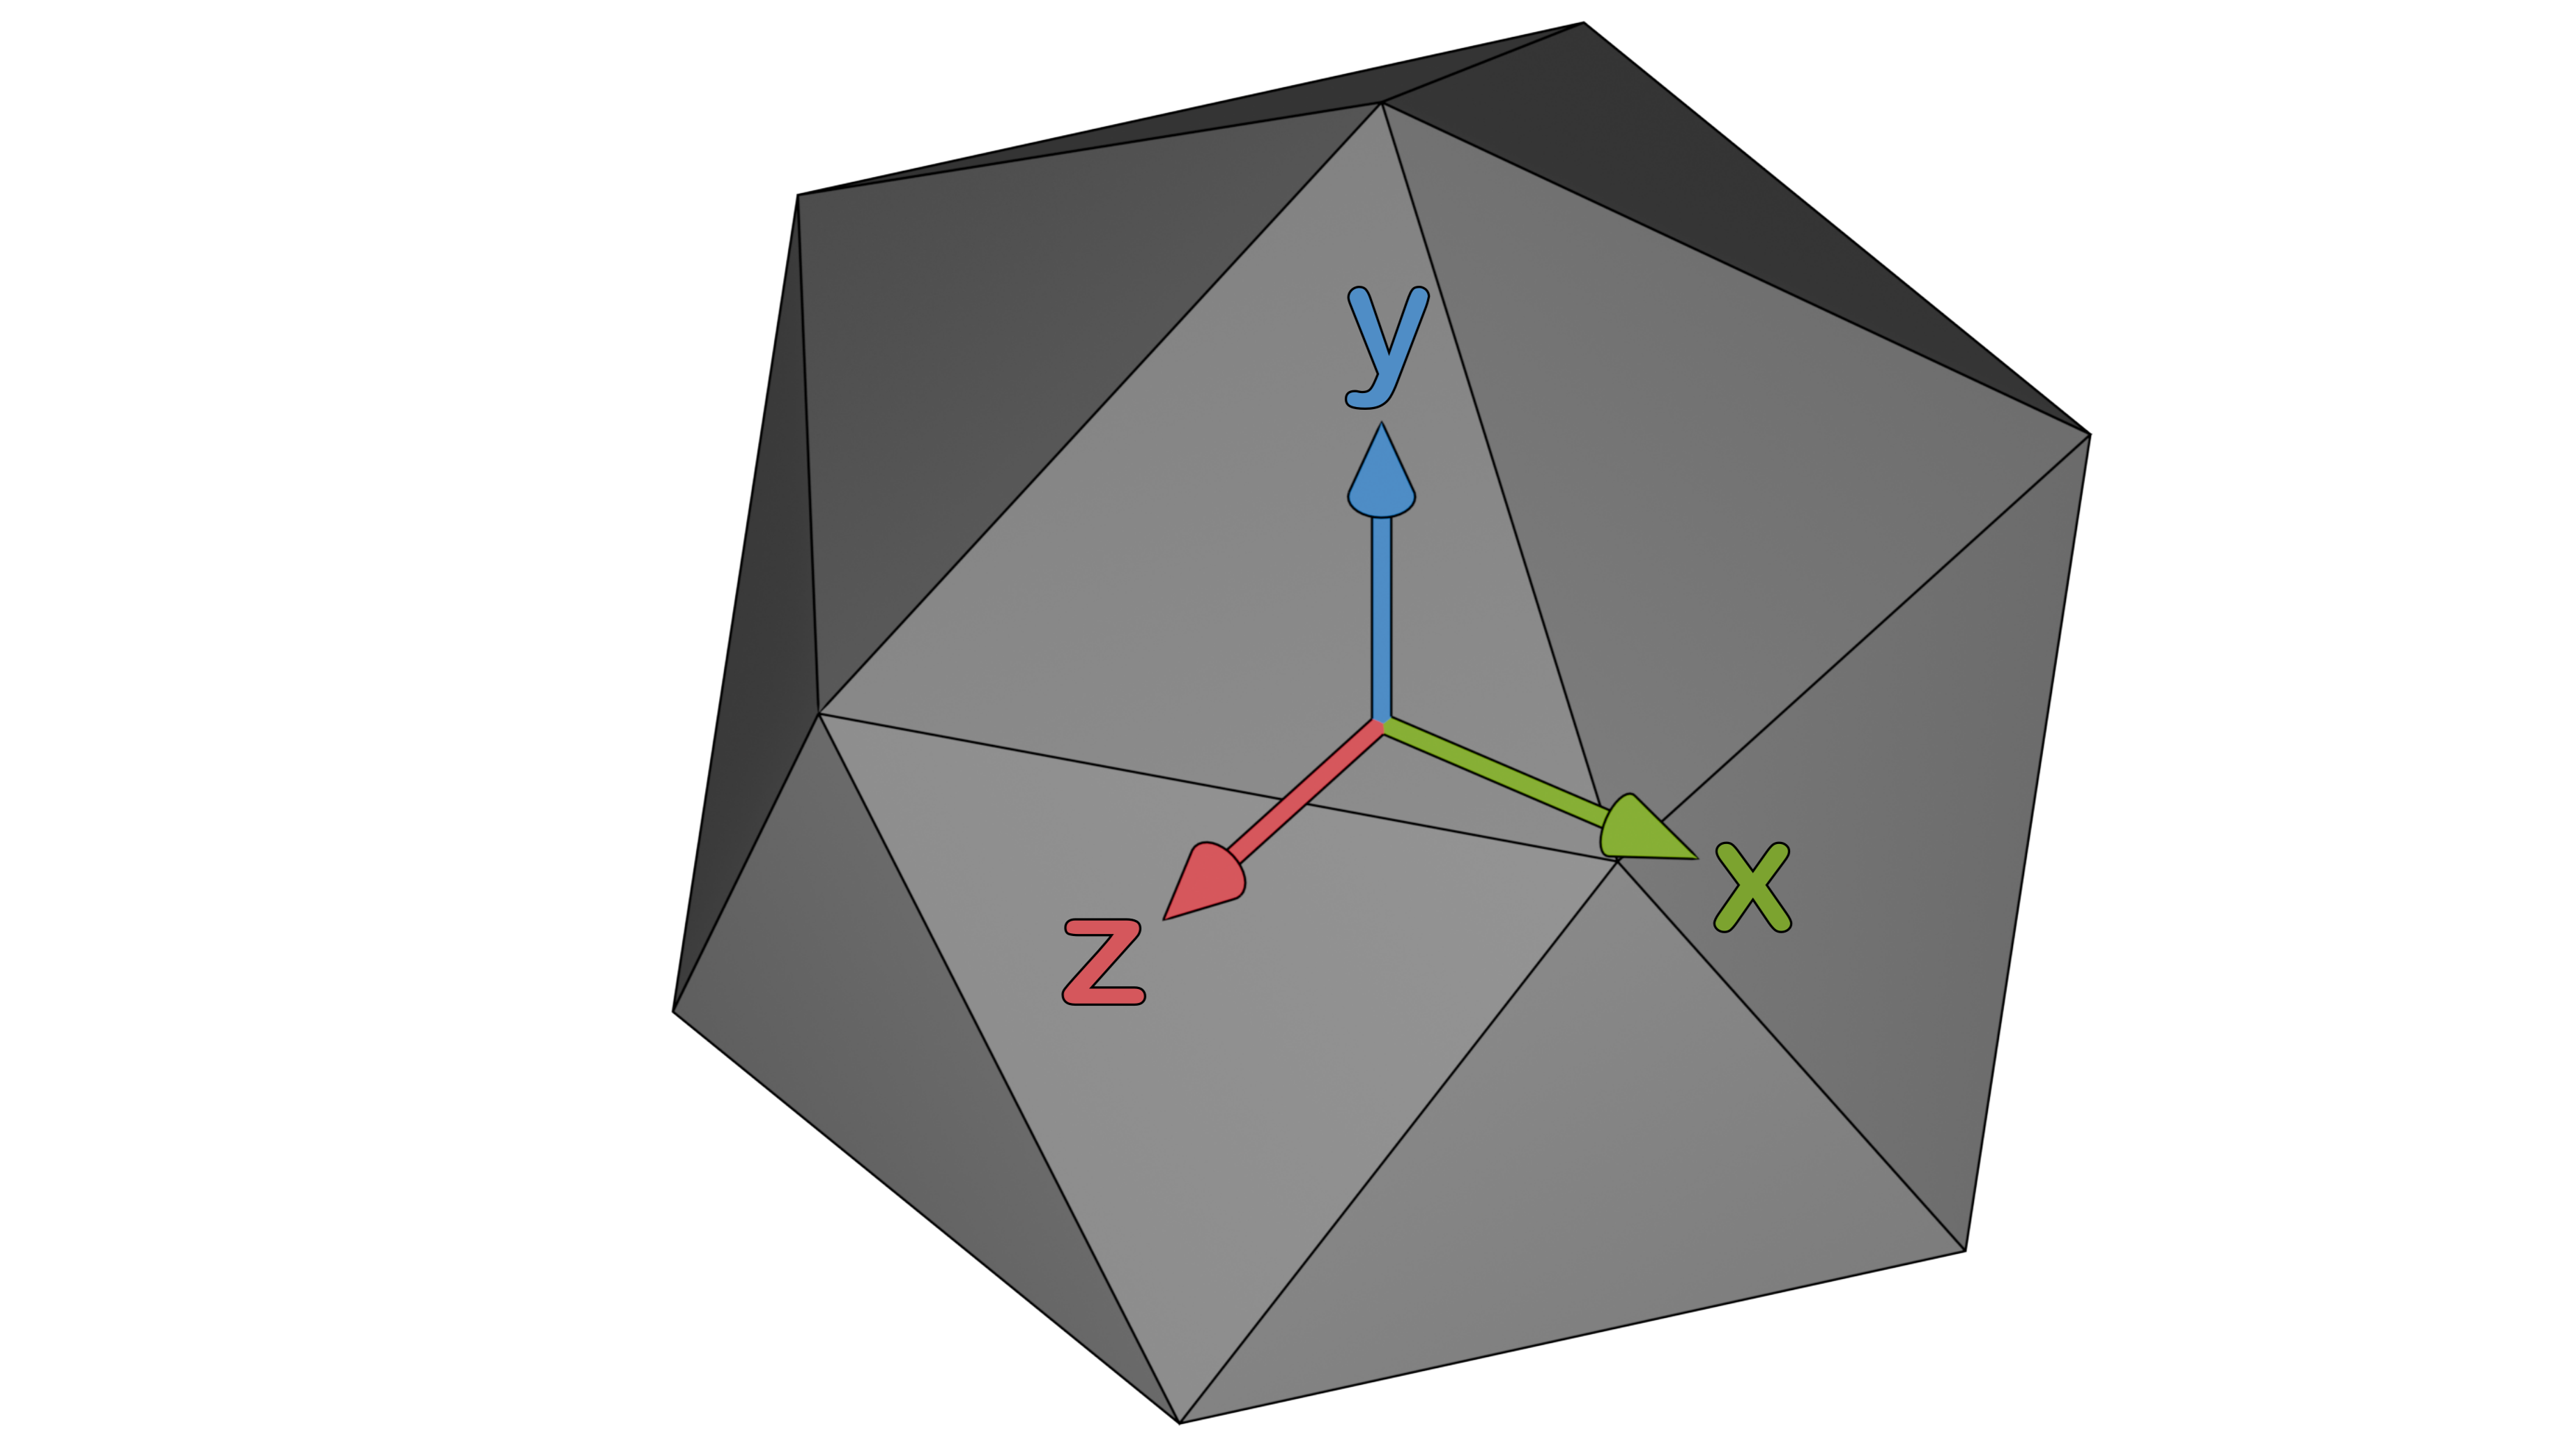
\includegraphics[width=0.8\textwidth]{assets/figures/second_phase/node/img_node_geometry.png}
    \label{fig:node_geometry}
    
\end{figure}
\vspace{-0.6\baselineskip}

            \paragraph{Nodo de control de transformación visual.}
            
                También denominado \textit{gizmo} o manipulador de transformación, fue implementado como una herramienta de asistencia visual que representa los ejes de transformación de un objeto tridimensional mediante tres flechas finitas orientadas en el sentido positivo de los ejes X, Y y Z, utilizada durante la edición de animaciones o posición de los nodos de escena tridimensionales (ver Figura \ref{fig:node_gizmo}).
            
                \begin{figure}[H]
    \caption{Nodo de control de transformación visual}
    \centering
    \borderedgraphics{assets/figures/second_phase/node/img_node_gizmo_text.png}
    \label{fig:node_gizmo}
\end{figure}
\fixvspace{1}

            \paragraph{Nodo de marcador.}
            
                Equivalente a un objetivo rastreable dentro de una sesión de realidad aumentada, implementa una clase encargada de administrar el seguimiento espacial de imágenes aumentadas detectadas mediante la cámara del dispositivo (ver Figura \ref{fig:uml_marker_inheritance}). 

                \begin{figure}[H]
    \caption{Clases heredadas del nodo marcador}
    \centering
    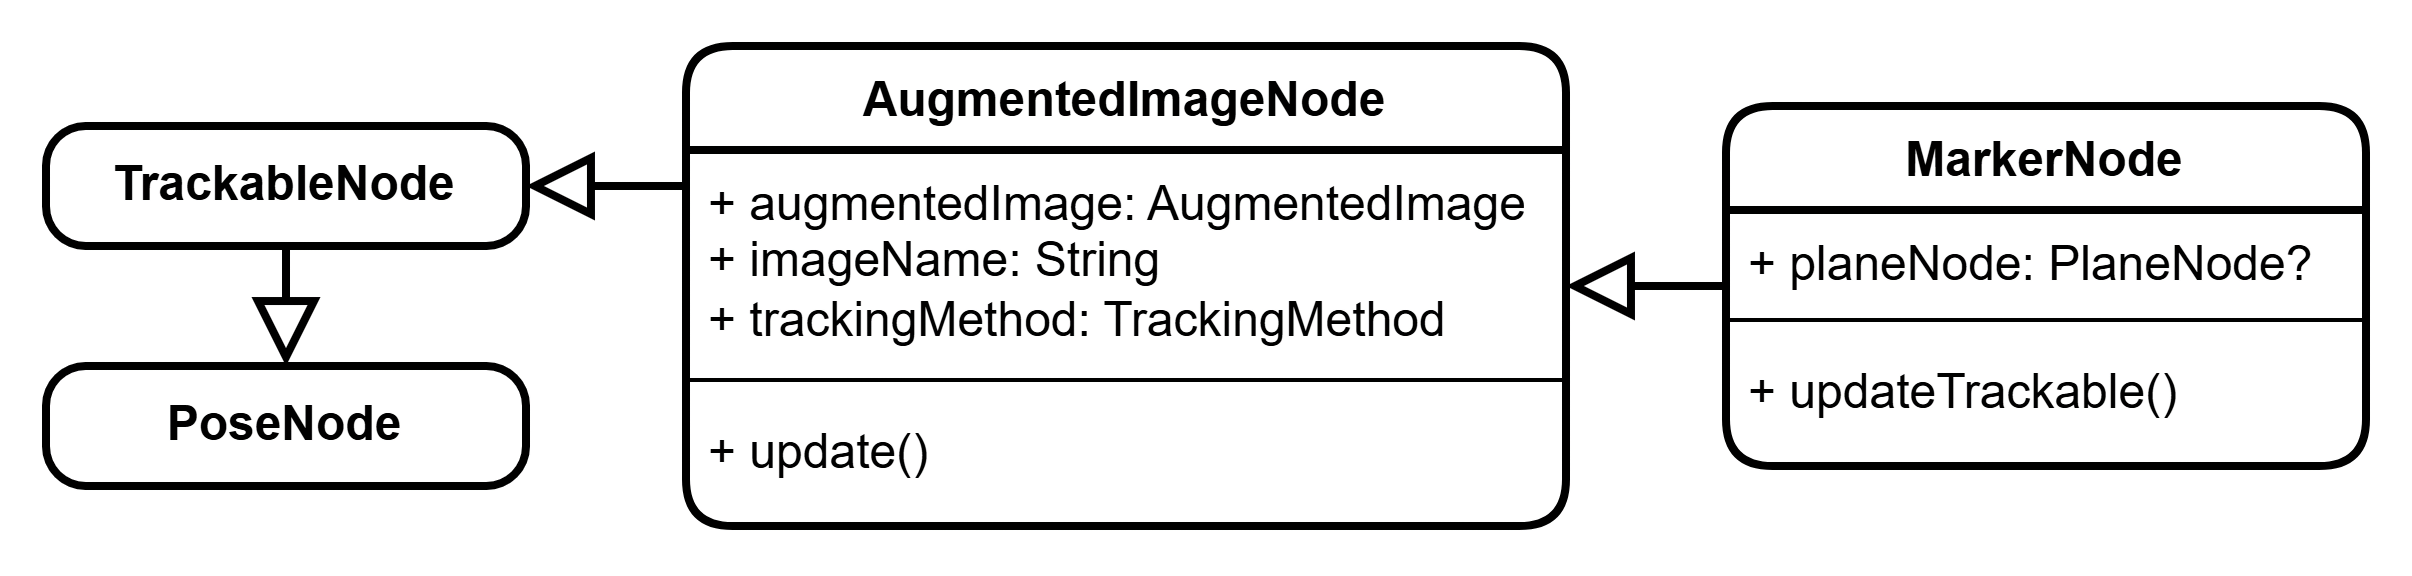
\includegraphics[width=\textwidth]{assets/figures/second_phase/diagram/img_uml_marker_inheritance.png}
    \label{fig:uml_marker_inheritance}
\end{figure}
\fixvspace{1}
            
                Este comportamiento permite obtener la transformación asociada a un marcador físico detectado dentro de la escena (ver Figura \ref{fig:node_augmented_image}) y utilizarla posteriormente para el reposicionamiento dinámico de modelos tridimensionales durante las sesiones de realidad aumentada.

                \begin{figure}[H]
    \caption{Nodo de marcador}
    \centering
    \borderedgraphics{assets/figures/second_phase/node/img_node_marker.png}
    \caption*{\textit{Nota}. \textnormal{La imagen sólo ilustra la transformación detectada de un marcador físico, este nodo no añade un nodo de control de transformación (\textit{gizmo}).}}
    \label{fig:node_augmented_image}
\end{figure}
\fixvspace{0.5}

                \subparagraph{Nodo de plano.}

                    Representa una geometría plana superpuesta al nodo de marcador, utilizado como representación visual del estado de seguimiento de una imagen aumentada detectada mediante la cámara del dispositivo. Usa un esquema de materiales basado en colores: verde para indicar seguimiento activo del marcador, amarillo para indicar pérdida temporal de seguimiento conservando la última posición detectada y rojo para indicar pérdida total tanto del seguimiento como de la última posición registrada del marcador (ver Figura \ref{fig:node_plane}).

                    \begin{figure}[H]
    \caption{Estados del nodo de marcador mediante planos}
    \centering
    \setlength{\tabcolsep}{0pt}
    \renewcommand{\arraystretch}{1.2}
    \begin{tabular}{
        |>{\centering\arraybackslash}m{(\textwidth - 4\arrayrulewidth) / 3}
        |>{\centering\arraybackslash}m{(\textwidth - 4\arrayrulewidth) / 3}
        |>{\centering\arraybackslash}m{(\textwidth - 4\arrayrulewidth) / 3}|
    }
        \hline

        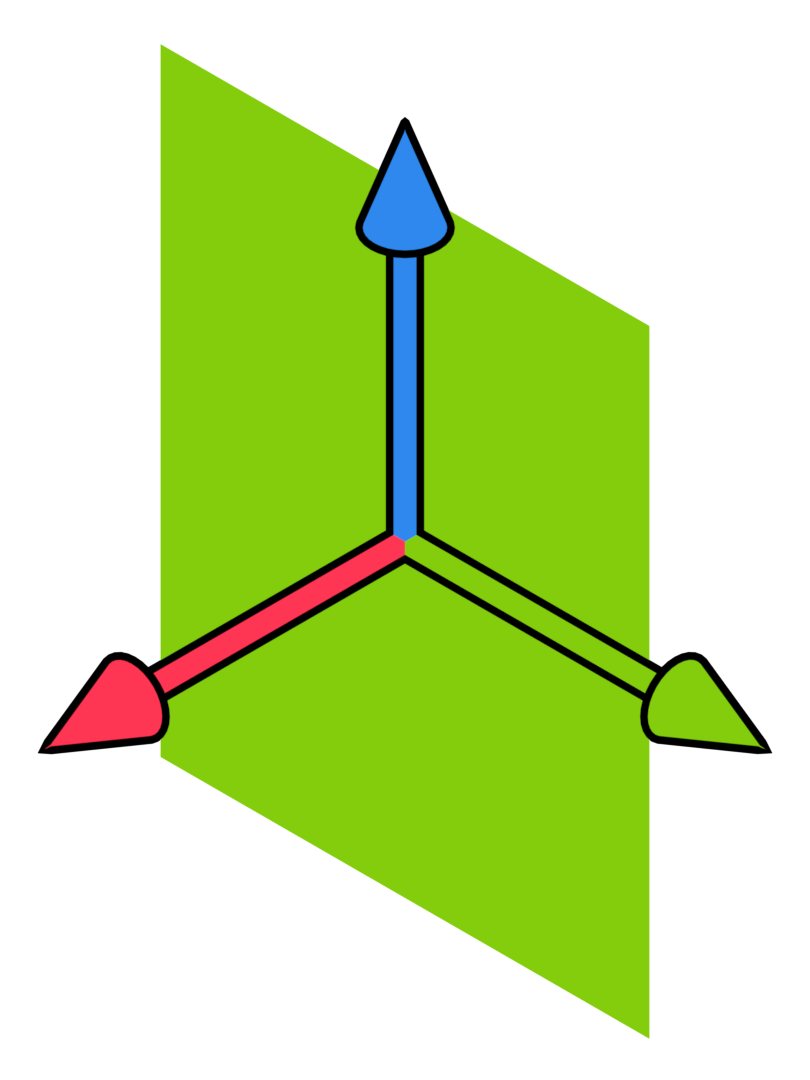
\includegraphics[width=(\textwidth - 4\arrayrulewidth) / 3]
        {assets/figures/second_phase/node/img_node_plane_green.png} &
            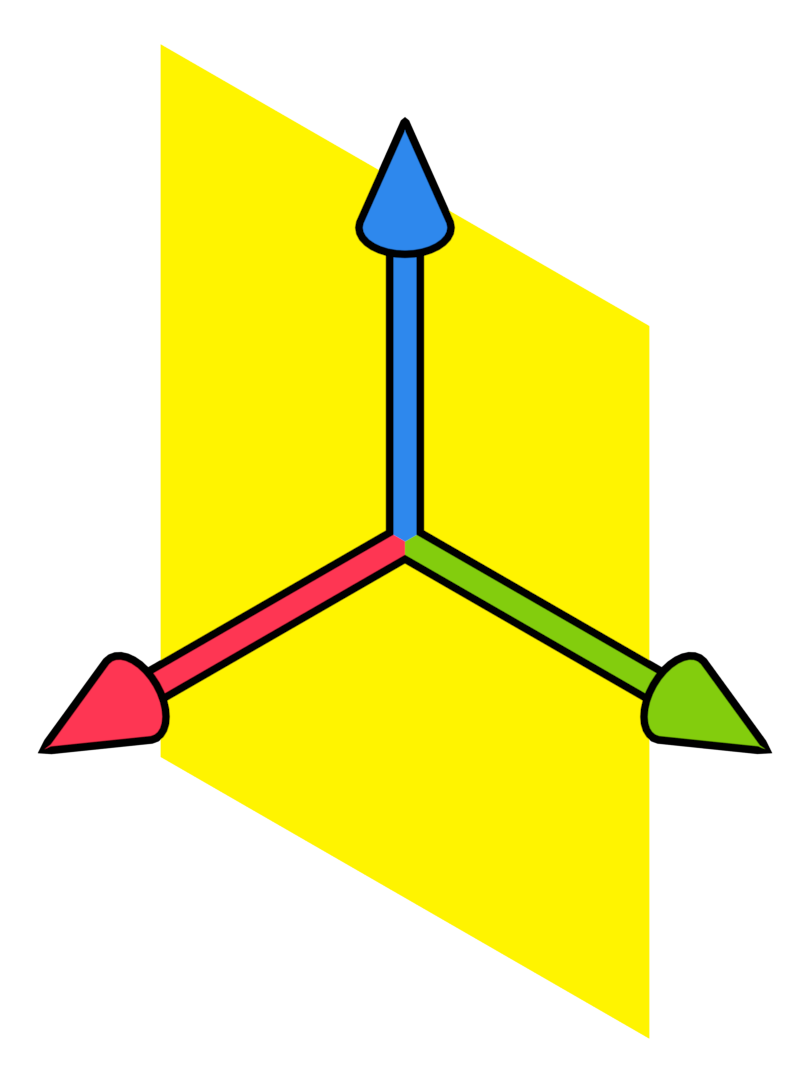
\includegraphics[width=(\textwidth - 4\arrayrulewidth) / 3]
        {assets/figures/second_phase/node/img_node_plane_yellow.png} &
                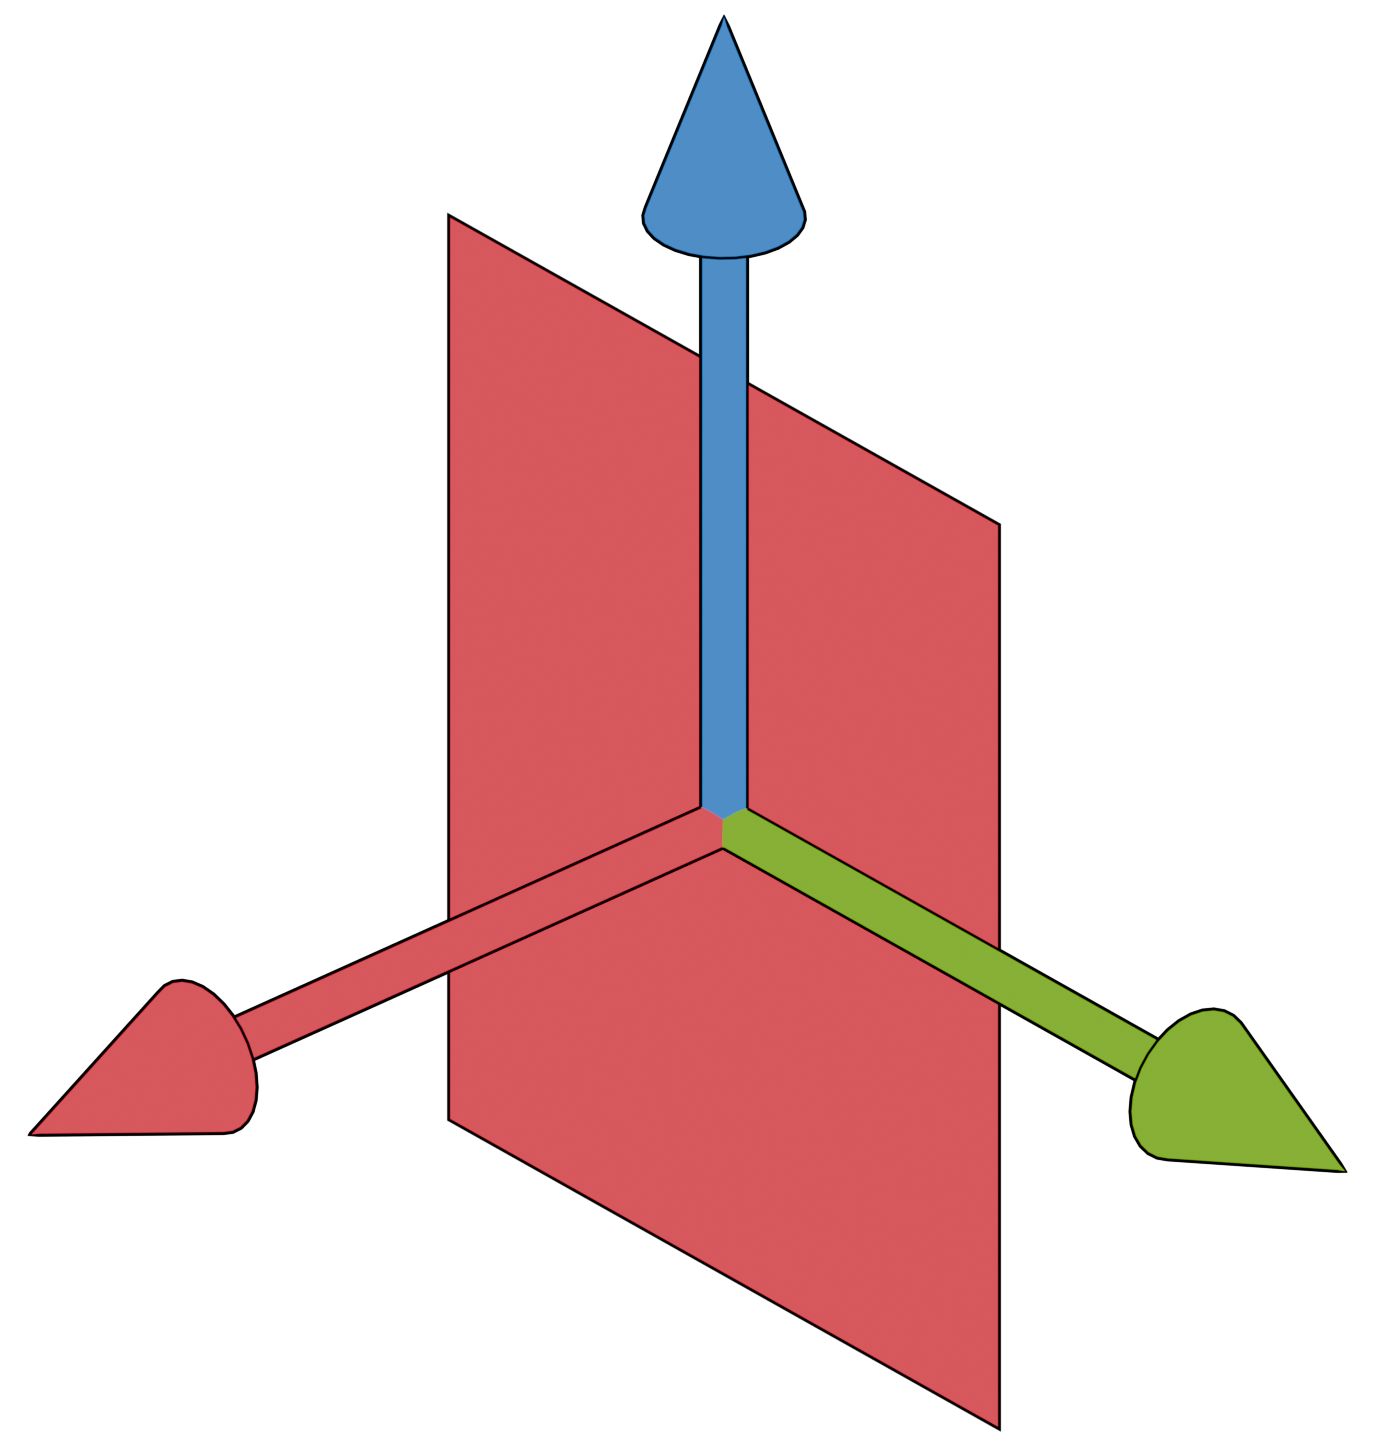
\includegraphics[width=(\textwidth - 4\arrayrulewidth) / 3]
        {assets/figures/second_phase/node/img_node_plane_red.png} \\

        \rule{0pt}{0.8cm}\small Seguimiento activo del marcador &
            \rule{0pt}{0.8cm}\small Pérdida temporal del seguimiento &
                \rule{0pt}{0.8cm}\small Pérdida total del seguimiento \\

        \hline
    \end{tabular}
    \label{fig:node_plane}
\end{figure}
\fixvspace{0}

            \paragraph{Nodo de caja.}
            
                También conocido como caja delimitadora, corresponde a la representación visual de selección de submodelos tridimensionales mediante un nodo geométrico de caja que envuelve y delimita el elemento seleccionado dentro de la escena de realidad aumentada (ver Figura \ref{fig:node_box}).

                \begin{figure}[H]
    \caption{Nodo de caja de selección}
    \centering
    \setlength{\tabcolsep}{0pt}
    \renewcommand{\arraystretch}{1.2}
    \begin{tabular}{
        |>{\centering\arraybackslash}m{(\textwidth - 3\arrayrulewidth) / 2}
        |>{\centering\arraybackslash}m{(\textwidth - 3\arrayrulewidth) / 2}|
    }
        \hline

        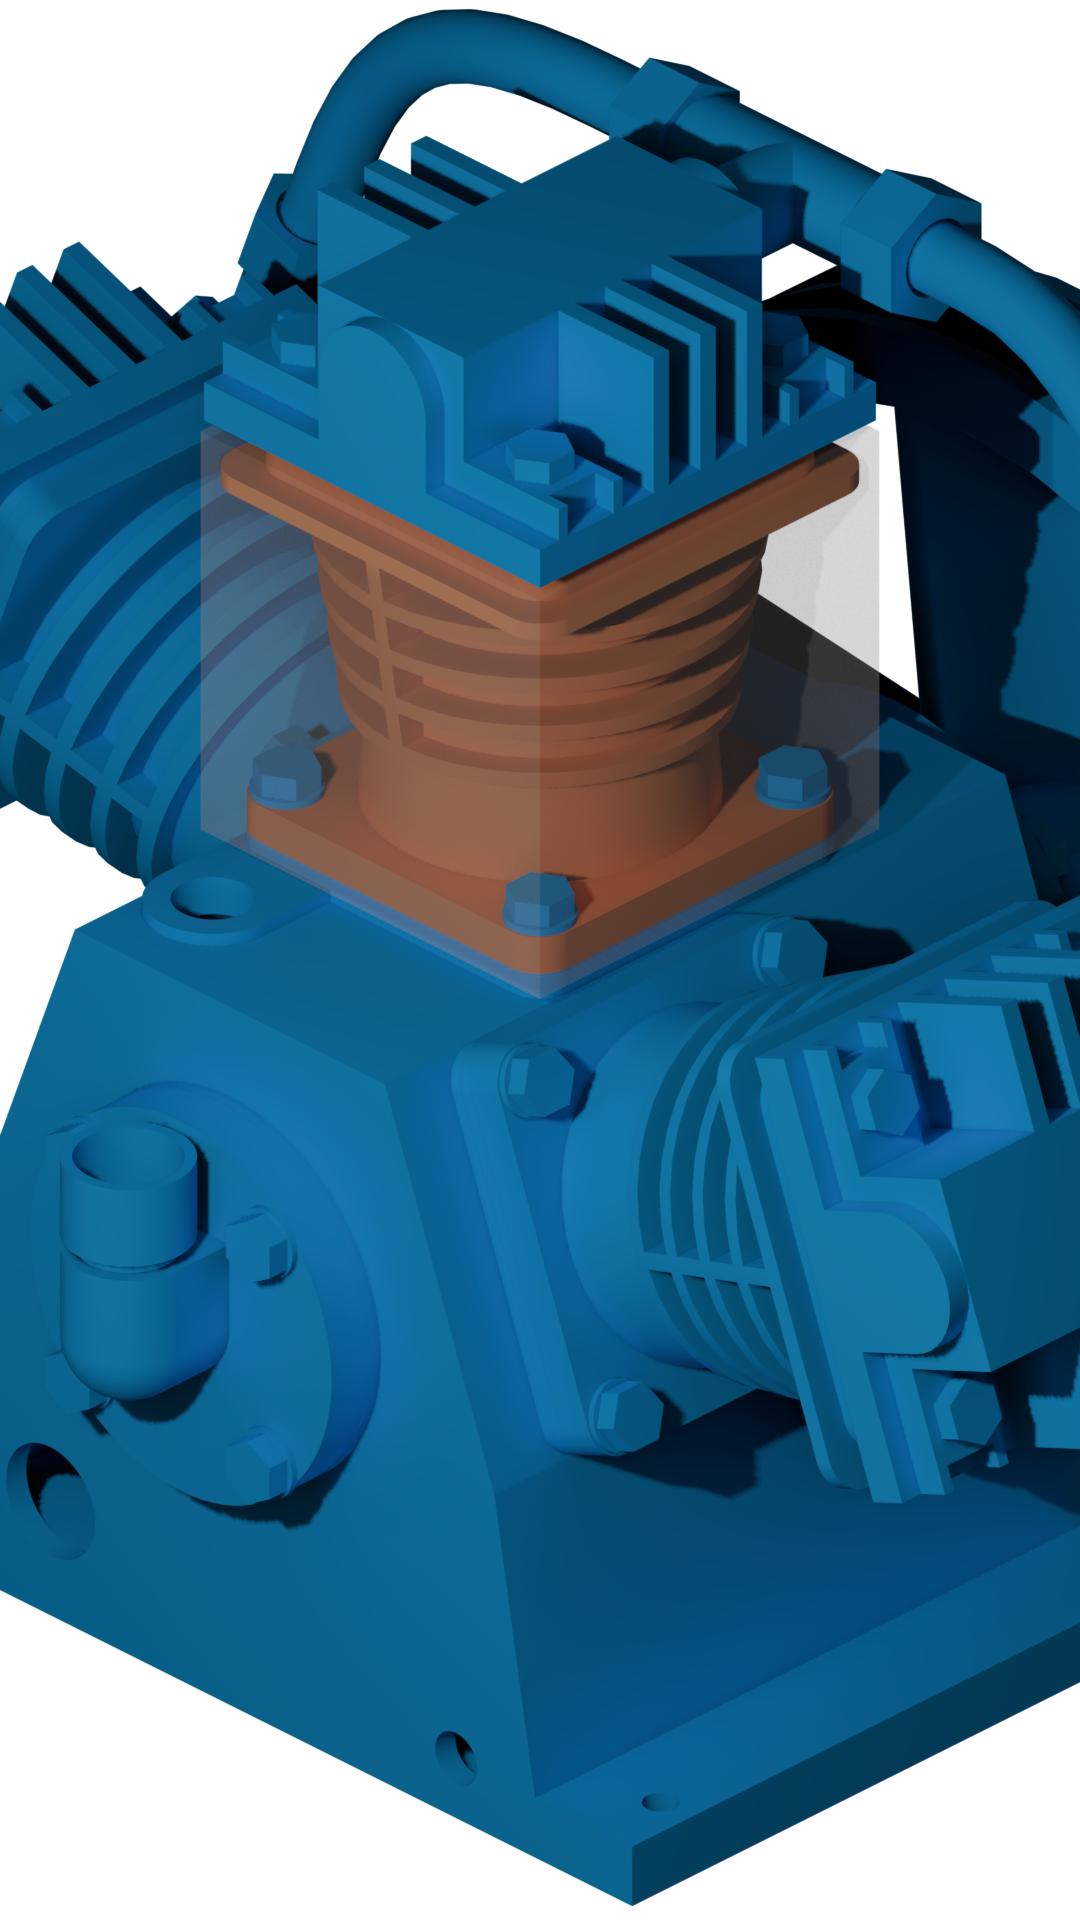
\includegraphics[width=(\textwidth - 3\arrayrulewidth) / 2]
        {assets/figures/second_phase/node/img_node_box_selection.png} &
            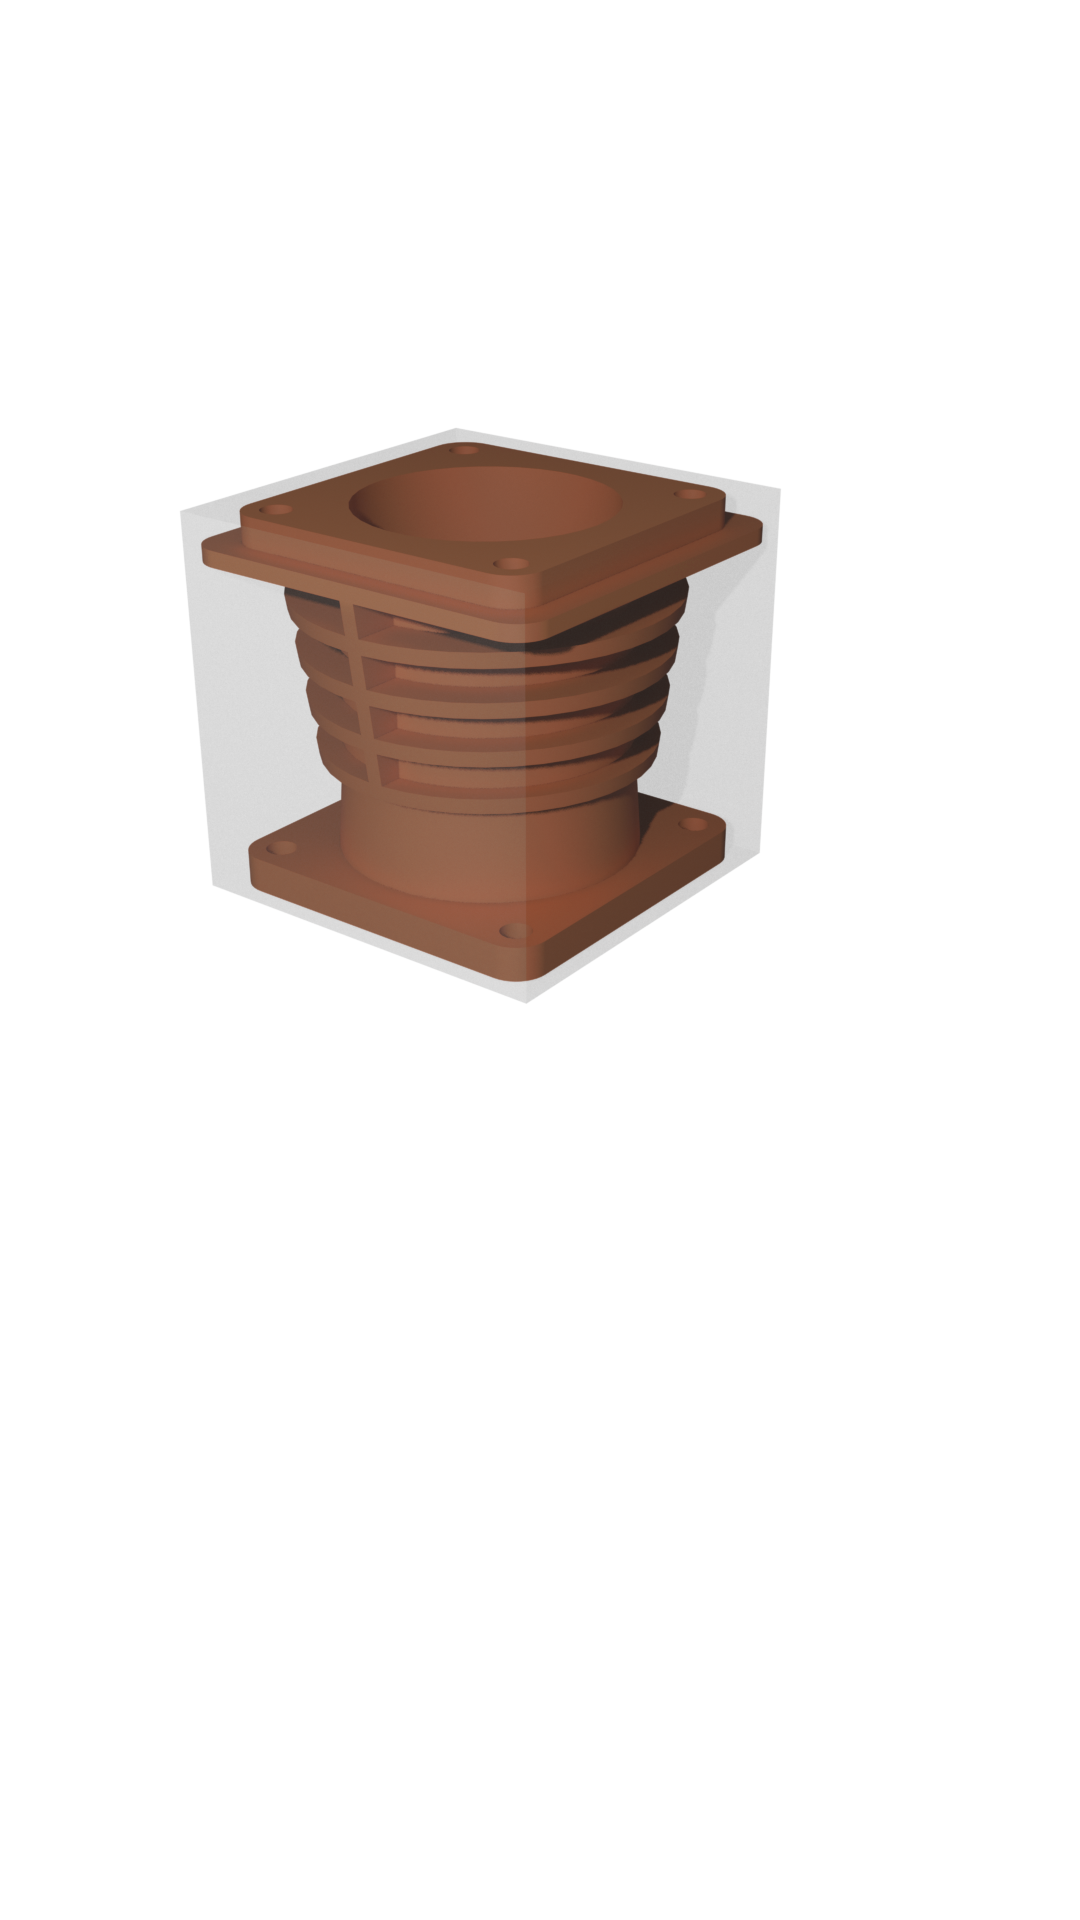
\includegraphics[width=(\textwidth - 3\arrayrulewidth) / 2]
        {assets/figures/second_phase/node/img_node_box_isolated.png} \\

        \small Selección de submodelo &
            \small Selección de submodelo aislada \\
        
        \hline
    \end{tabular}
    \label{fig:node_box}
\end{figure}
\fixvspace{0}

            \paragraph{Nodo de eje.}
            
                Implementado como guía visual de transformación que representa espacialmente uno de los ejes X, Y o Z (ver Figura \ref{fig:node_axes}). Utilizados durante la manipulación de posición de modelos tridimensionales.

                \begin{figure}[H]

    \caption{Nodos de eje infinitos}
    \centering

    \setlength{\tabcolsep}{0pt}
    \renewcommand{\arraystretch}{1}

    \begin{tabular}{
        |>{\centering\arraybackslash}m{1\textwidth}|
    }
        \hline

        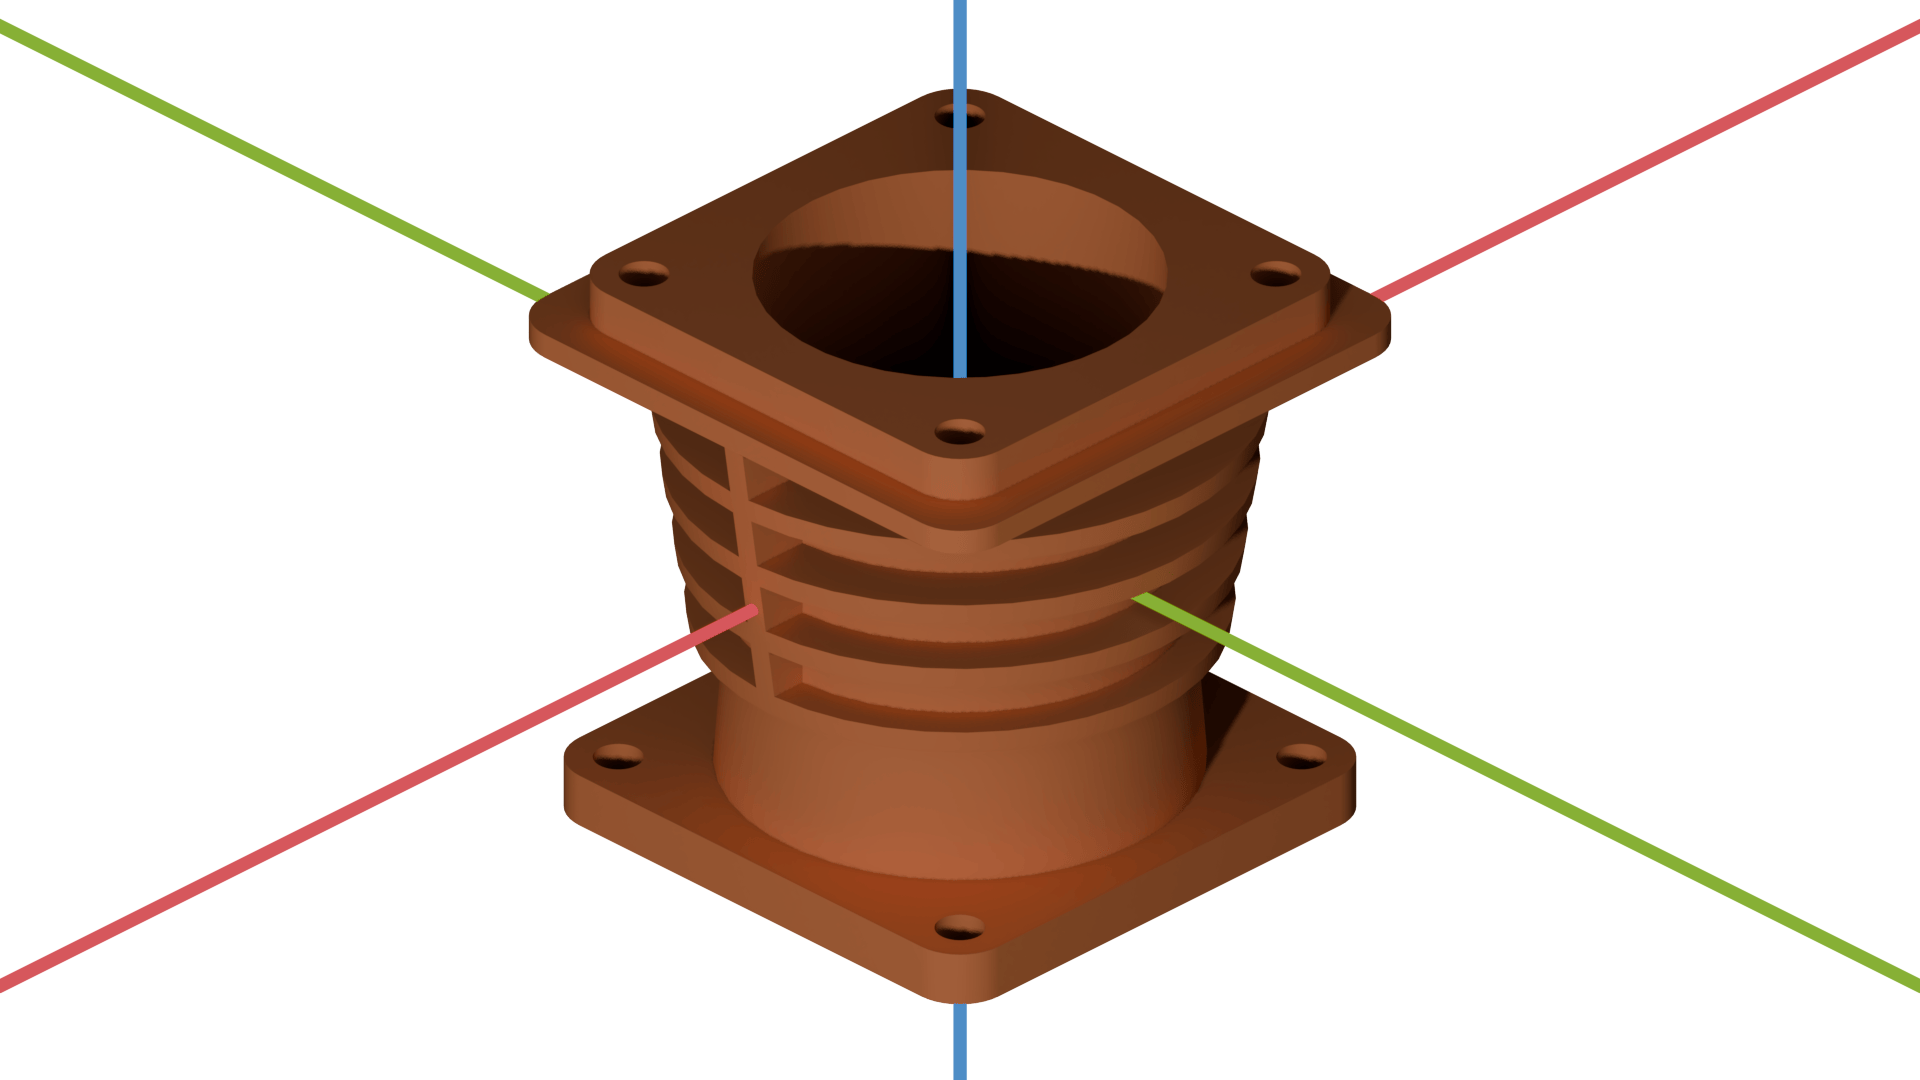
\includegraphics[width=1\textwidth]
        {assets/figures/second_phase/node/img_node_axes.png}

        \\ \hline
    \end{tabular}
    \label{fig:node_axes}
    
\end{figure}
\fixvspace{0}

        \subsubsection{Nodos de escena tridimensionales.}

            Los nodos de escena representan el contenido visual tridimensional cargado desde archivos con formato \textit{.glb}.

            \paragraph{Nodo de modelo.}

                Representa un modelo 3D con sus partes en su totalidad (ver Figura \ref{fig:node_model}) cargado desde un archivo con formato \textit{.glb}. Este nodo mantiene una referencia a los objetos de sus partes renderizables a través de la propiedad \textit{renderableNodes}.

                \begin{figure}[H]
    \caption{Nodo de modelo}
    \centering
    \borderedgraphics{assets/figures/second_phase/node/img_node_model.png}
    \label{fig:node_model}
\end{figure}
\fixvspace{1}

                \subparagraph{Nodo de renderizable.}

                    Representa una malla renderizable individual (submodelo) extraída de un nodo de modelo, correspondiente a un \textit{renderableNode} identificable dentro del archivo \textit{.glb}, al cual se le pueden asignar texturas y materiales de forma individual. Al iniciar la escena es reparentado desde el nodo de modelo a un nodo dedicado a la corrección espacial, permitiendo su manipulación, aplicación de materiales y animación de forma independiente. Sin embargo este preserva el vínculo desde su nodo padre mediante la propiedad de \textit{renderableNodes}.

                    %agregar imagen TODO:

        \subsubsection{Nodos de jerarquía espacial}

            Los nodos de jerarquía espacial estructuran la organización de los modelos tridimensionales dentro de la escena mediante una cadena de parentesco: el nodo de origen agrupa los contenedores del modelo, cada contenedor corrige el centro espacial del modelo y agrupa sus pivotes, y cada pivote corrige el centro espacial de un renderizable individual. Esta jerarquía permite tanto el reposicionamiento en bloque de todos los modelos insertados en la escena de realidad aumentada mediante un marcador, como la manipulación independiente de cada renderizable (ver Figura \ref{fig:uml_node_hierarchy}).

            \begin{figure}[H]
    \caption{Jerarquía completa de nodos}
    \centering
    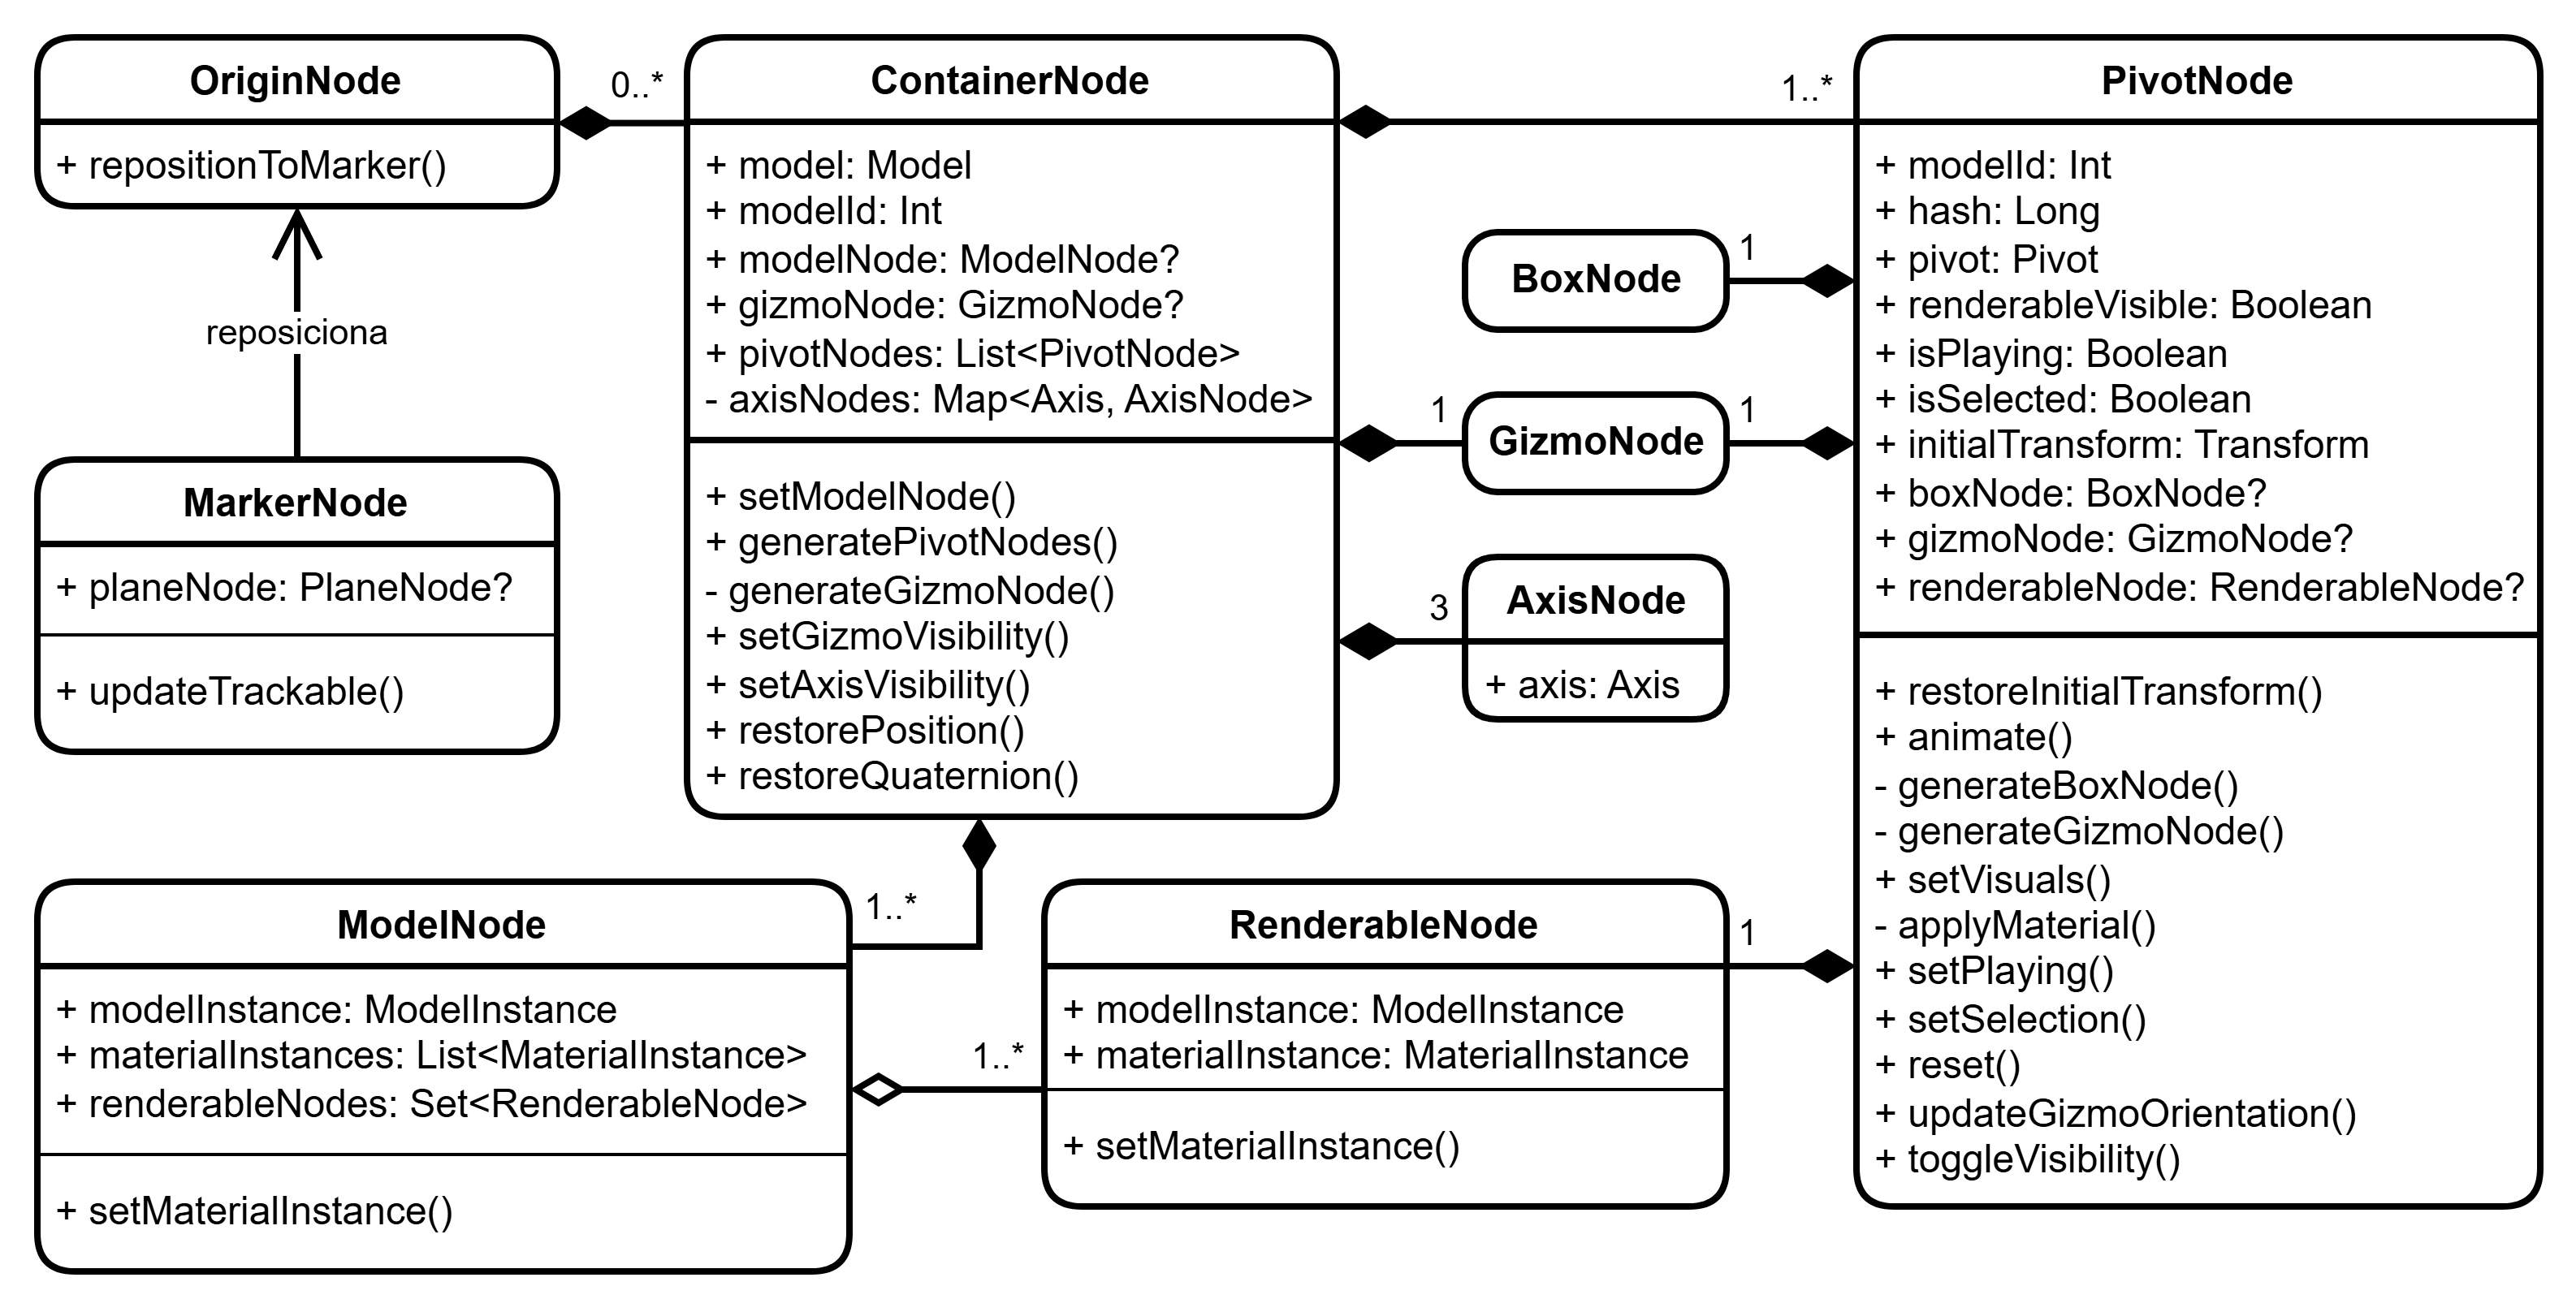
\includegraphics[width=\textwidth]{assets/figures/second_phase/diagram/img_uml_node_hierarchy.png}
    \label{fig:uml_node_hierarchy}
\end{figure}
\fixvspace{1}

            Cada nodo mantiene una transformación local relativa a su nodo padre, permitiendo construir estructuras espaciales jerárquicas y conservar relaciones de posición y orientación entre los distintos elementos de la escena.

            \paragraph{Nodo de cámara de realidad aumentada.}

                Representa una cámara virtual desde la cual se observa la perspectiva de la escena de realidad aumentada. Su posición y rotación están ligadas al movimiento físico del dispositivo en el mundo real, controladas por ARCore, siendo la vista principal donde se renderiza la escena tridimensional (ver Figura \ref{fig:node_camera}).

                \begin{figure}[H]
    \caption{Nodo de cámara de realidad aumentada}
    \centering
    \borderedgraphics{assets/figures/second_phase/node/img_node_camera.png}
    \label{fig:node_camera}
\end{figure}
\fixvspace{1}

                % agregar imagen comparativa de la escena vista mediante el dispositivo a el mundo real TODO:

            \paragraph{Nodo de origen.}

                Actúa como raíz de la jerarquía de los modelos en la escena, agrupando nodos de contenedor como hijos directos, permitiendo el reposicionamiento en bloque de sus descendientes a partir del desplazamiento calibrado respecto a un nodo de marcador almacenado en la base de datos.

            \paragraph{Nodo de contenedor.}

                Contiene únicamente un nodo de modelo como hijo directo (ver Figura \ref{fig:node_container}), corrigiendo el centro espacial real del modelo cuando el origen geométrico exportado no coincide con el centro visual de la malla, y agrupando todos sus nodos de pivote hijos. Adicionalmente, permite anexar bajo demanda nodos de asistencia visual desde su centro corregido: un nodo de control de transformación visual (\textit{gizmo}) y hasta tres nodos de eje independientes, uno por cada eje X, Y y Z.

                \begin{figure}[H]
    \caption{Nodos contenedores de modelos}
    \centering
    \borderedgraphics{assets/figures/second_phase/node/img_node_container.png}
    \caption*{\textit{Nota}. \textnormal{Cada modelo es cargado de un archivo .glb diferente}}
    \label{fig:node_container}
\end{figure}
\fixvspace{0.5}

            \paragraph{Nodo de pivote.}

                Contiene únicamente un nodo renderizable o submodelo como hijo directo (ver Figura \ref{fig:node_pivots}), cumpliendo una función análoga al nodo de contenedor sobre cada renderizable individual. Es hijo del nodo de contenedor correspondiente a su modelo. De igual forma, permite anexar bajo demanda un nodo de control de transformación visual (\textit{gizmo}) y un nodo de caja delimitadora, ambos anclados desde el centro corregido del renderizable.

                \begin{figure}[H]
    \caption{Nodos pivotes de renderizables de un modelo}
    \centering
    \borderedgraphics{assets/figures/second_phase/node/img_node_pivots.png}
    \caption*{\textit{Nota}. \textnormal{Se utiliza una versión simplificada del modelo con un número reducido de submodelos para ilustrar con mayor claridad la estructura de nodos pivote.}}
    \label{fig:node_pivots}
\end{figure}
\fixvspace{0.5}

        \subsubsection{Sesión de realidad aumentada}

            Una sesión de ARCore es la clase encargada de gestionar el ciclo de vida y el estado del sistema de realidad aumentada. Este proceso comprende desde la configuración e inicialización del entorno, hasta su ejecución activa, etapa en la cual se llevan a cabo las tareas de detección e interacción.
            
            \paragraph{Configuración inicial.}
            
                La configuración inicial define los parámetros que controlan la experiencia antes de iniciar el procesamiento de la escena de realidad aumentada. En este proyecto la configuración inicial se establece mediante el bloque de código del Apéndice \ref{apc:session_configuration}, el cual ajusta los siguientes parámetros:

            \begin{enumerate}
                
                \item Enfoque automático: Activado para que la cámara mantenga la nitidez sin intervención del usuario.

                \item Estimación de luz: Desactivada porque la aplicación utiliza principalmente materiales que no interactúan con la luz o tienen un sombreado estilo cartoon en donde la iluminación real tiene un impacto limitado y controlado.

                \item Ubicación instantánea: Desactivada con el fin de evitar estimaciones geométricas preliminares imprecisas y priorizar el procesamiento en los algoritmos principales de la aplicación.

                \item Modo de profundidad: Habilitado si el dispositivo es compatible, para obtener un mapa de profundidad más preciso.
                
                \item Búsqueda de planos: Activada para brindar una mejor experiencia de usuario (UX). Permitiendo visualizar una nube de puntos, confirmando visualmente que ARCore está funcionando.

            \end{enumerate}

    \subsection{Diseño de las interfaces gráficas}

        El diseño de la interfaz gráfica se desarrolló con el objetivo de proporcionar una experiencia de usuario consistente, intuitiva y adaptada a las necesidades identificadas durante la fase de requerimientos y restricciones. Para ello, se definió un sistema de diseño basado en componentes reutilizables y patrones de interacción uniformes, buscando mantener una apariencia homogénea en toda la aplicación, facilitar la navegación y simplificar la incorporación de nuevas funcionalidades.

        La interfaz del aplicativo está conformada por un conjunto de pantallas organizadas según el flujo de navegación de la Figura \ref{fig:uml_navigation_state}. Asimismo, incorpora componentes reutilizables que mantienen la consistencia visual y funcional entre las diferentes secciones del sistema. En los siguientes apartados se describen los principales componentes de la interfaz y la organización de las pantallas que conforman el aplicativo.

        \subsubsection{Diseño de los componentes comunes}

            Con el propósito de mantener la consistencia visual y funcional del aplicativo, se definió un conjunto de componentes reutilizables empleados en múltiples pantallas. Estos componentes fueron diseñados siguiendo una misma línea gráfica, permitiendo un comportamiento uniforme durante la interacción del usuario.

            Entre los componentes desarrollados se encuentran botones con iconografía, tarjetas con imagen principal para representar recursos relevantes, barras superiores para navegación, barras superiores con función de búsqueda integrada, controles de filtrado para la organización de contenidos y botones con indicadores numéricos utilizados para mostrar cantidades o estados de determinados elementos (ver Apéndice \ref{apc:common_components}). La reutilización de estos componentes facilita el mantenimiento de la interfaz y mejora la experiencia de uso al conservar patrones de interacción familiares para el usuario.

        \subsubsection{Diseño de las pantallas de la navegación principal}

            Las pantallas de la navegación principal constituyen el punto de acceso a las funcionalidades más importantes de la aplicación. Su diseño prioriza el acceso rápido a las funciones de mayor frecuencia de uso, permitiendo al usuario desplazarse de forma intuitiva entre los diferentes módulos del sistema mediante una estructura de navegación consistente.

            \paragraph{La pantalla de escáner}

                permite acceder a la información de una máquina mediante el reconocimiento de uno de sus marcadores físicos. Para ello, la interfaz prioriza el uso de la cámara del dispositivo y presenta únicamente los controles necesarios para iniciar el proceso de detección, reduciendo los elementos visuales que puedan interferir durante la captura.

                \begin{figure}[H]
    \caption{Pantalla de escáner de marcadores}
    \centering
    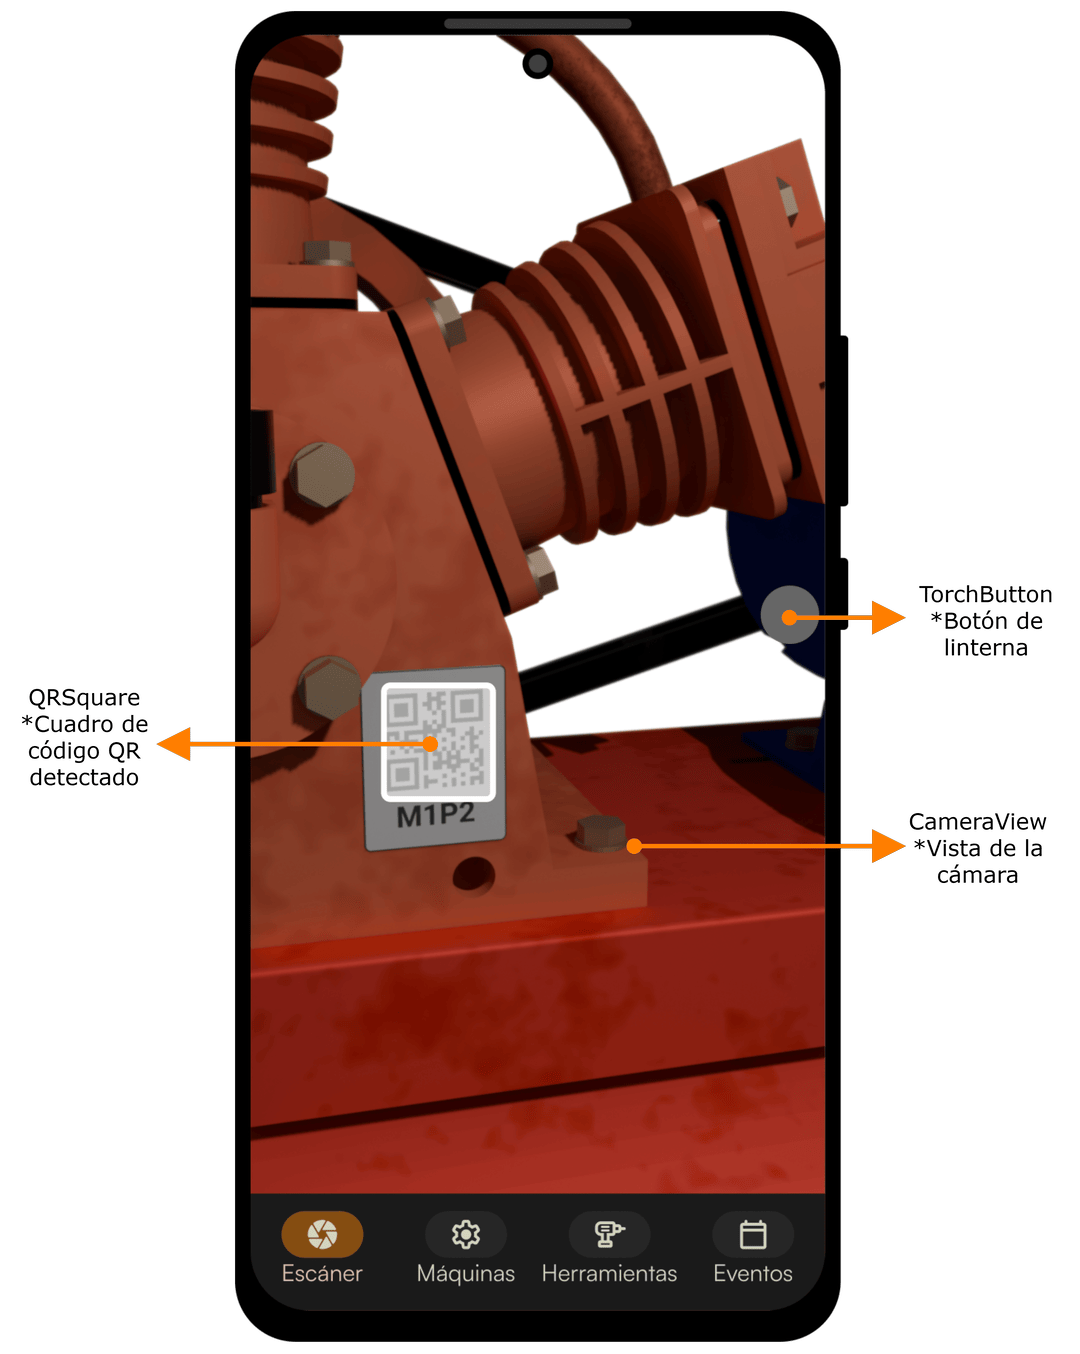
\includegraphics[height=12cm]{assets/figures/second_phase/screen/img_screen_scanner.png}
    \label{fig:screen_scanner}
\end{figure}

                Como se observa en la Figura \ref{fig:screen_scanner}, una vez detectado el marcador, el usuario puede acceder a la información de la máquina seleccionando el cuadro de reconocimiento que se superpone sobre el código QR identificado.

            \paragraph{La pantalla de máquinas}

                reúne el listado de equipos registrados dentro del sistema, permitiendo al usuario localizar rápidamente una máquina específica.

                \begin{figure}[H]
    \caption{Pantalla de listado de máquinas}
    \centering
    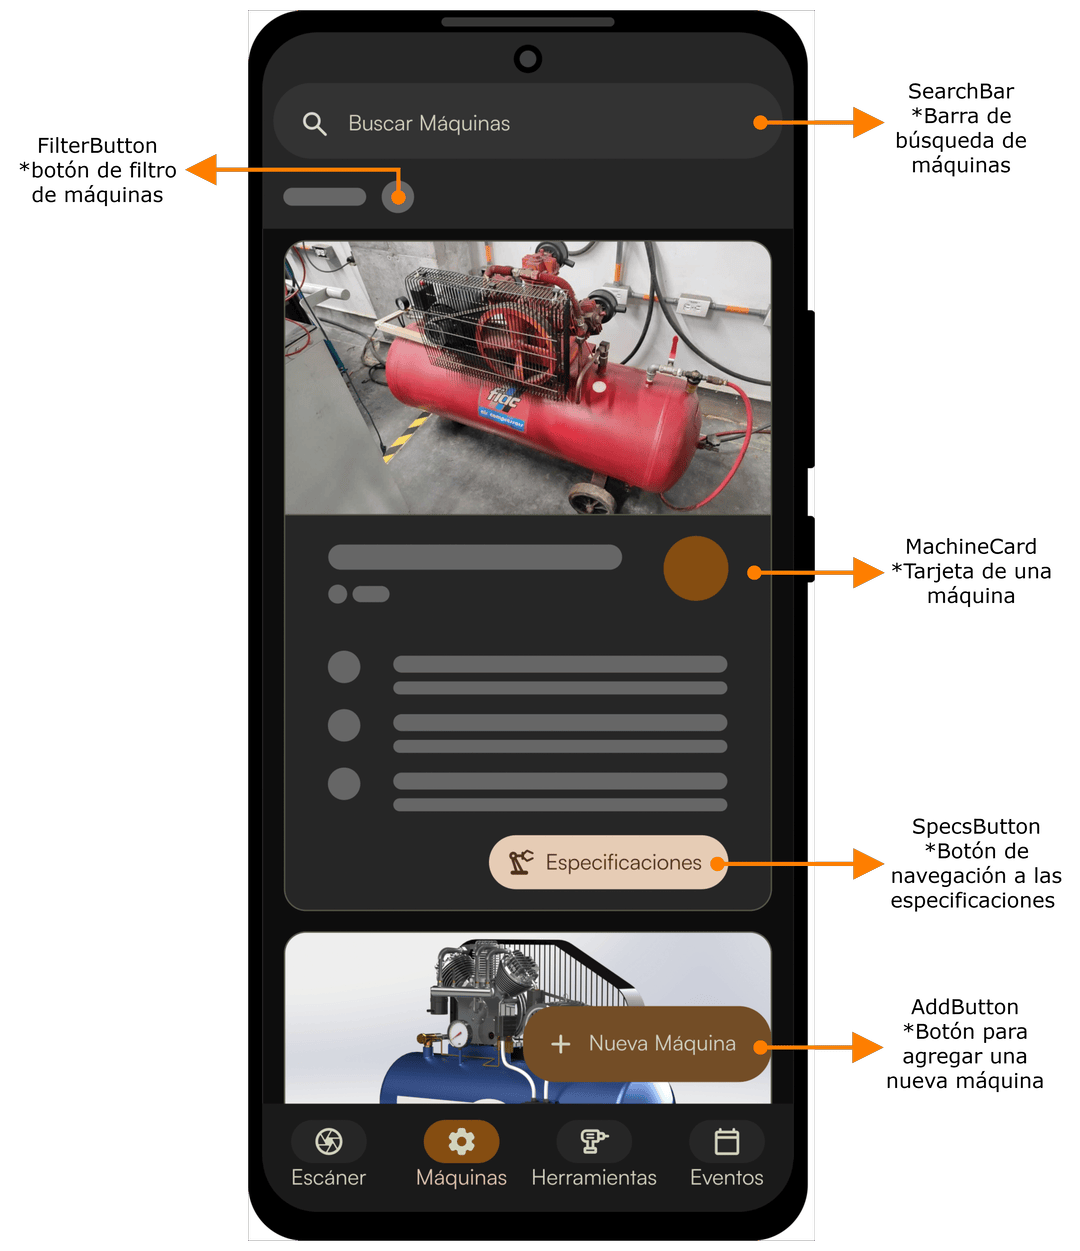
\includegraphics[height=12cm]{assets/figures/second_phase/screen/img_screen_machines.png}
    \label{fig:screen_machines}
\end{figure}

                La Figura \ref{fig:screen_machines} muestra una interfaz organizada mediante tarjetas que representan cada equipo, complementadas con herramientas de búsqueda y filtrado que facilitan la exploración del inventario de máquinas.

            \paragraph{La pantalla de herramientas}

                permite administrar las herramientas disponibles para el usuario dentro del aplicativo, las cuales podrán asociarse posteriormente a las operaciones definidas en las actividades de mantenimiento.

                \begin{figure}[H]
    \caption{Pantalla de listado de herramientas}
    \centering
    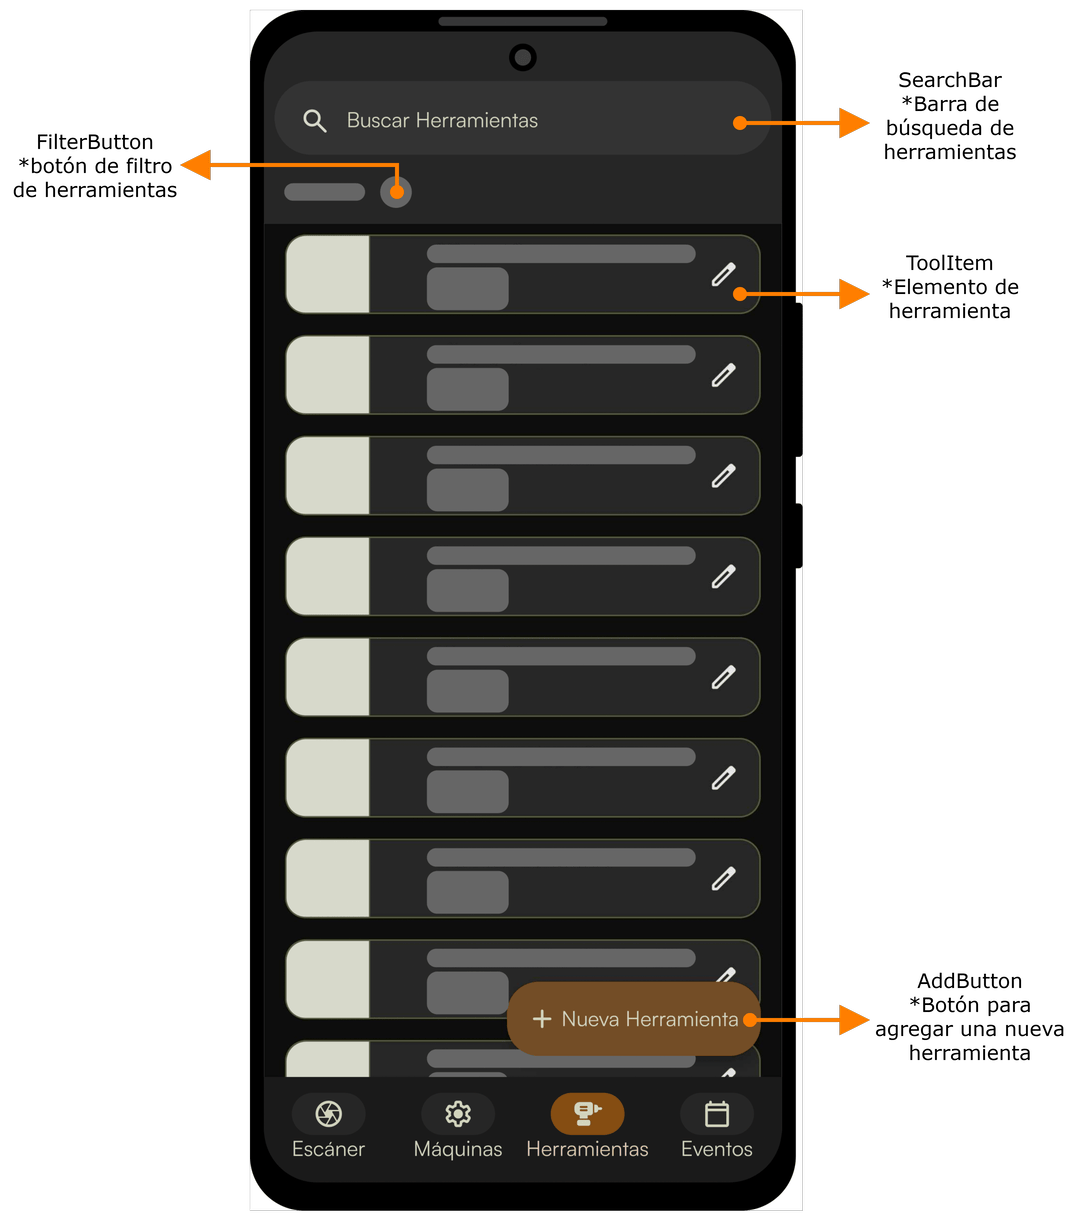
\includegraphics[height=12cm]{assets/figures/second_phase/screen/img_screen_tools.png}
    \label{fig:screen_tools}
\end{figure}

                Como se aprecia en la Figura \ref{fig:screen_tools}, la interfaz organiza las herramientas registradas en un listado que facilita su consulta y administración antes de ser utilizadas durante la configuración de las actividades.

            \paragraph{La pantalla de eventos}

                centraliza las actividades programadas y el historial de intervenciones realizadas sobre las máquinas registradas en el sistema.

                \begin{figure}[H]
    \caption{Pantalla de cronograma de eventos}
    \centering
    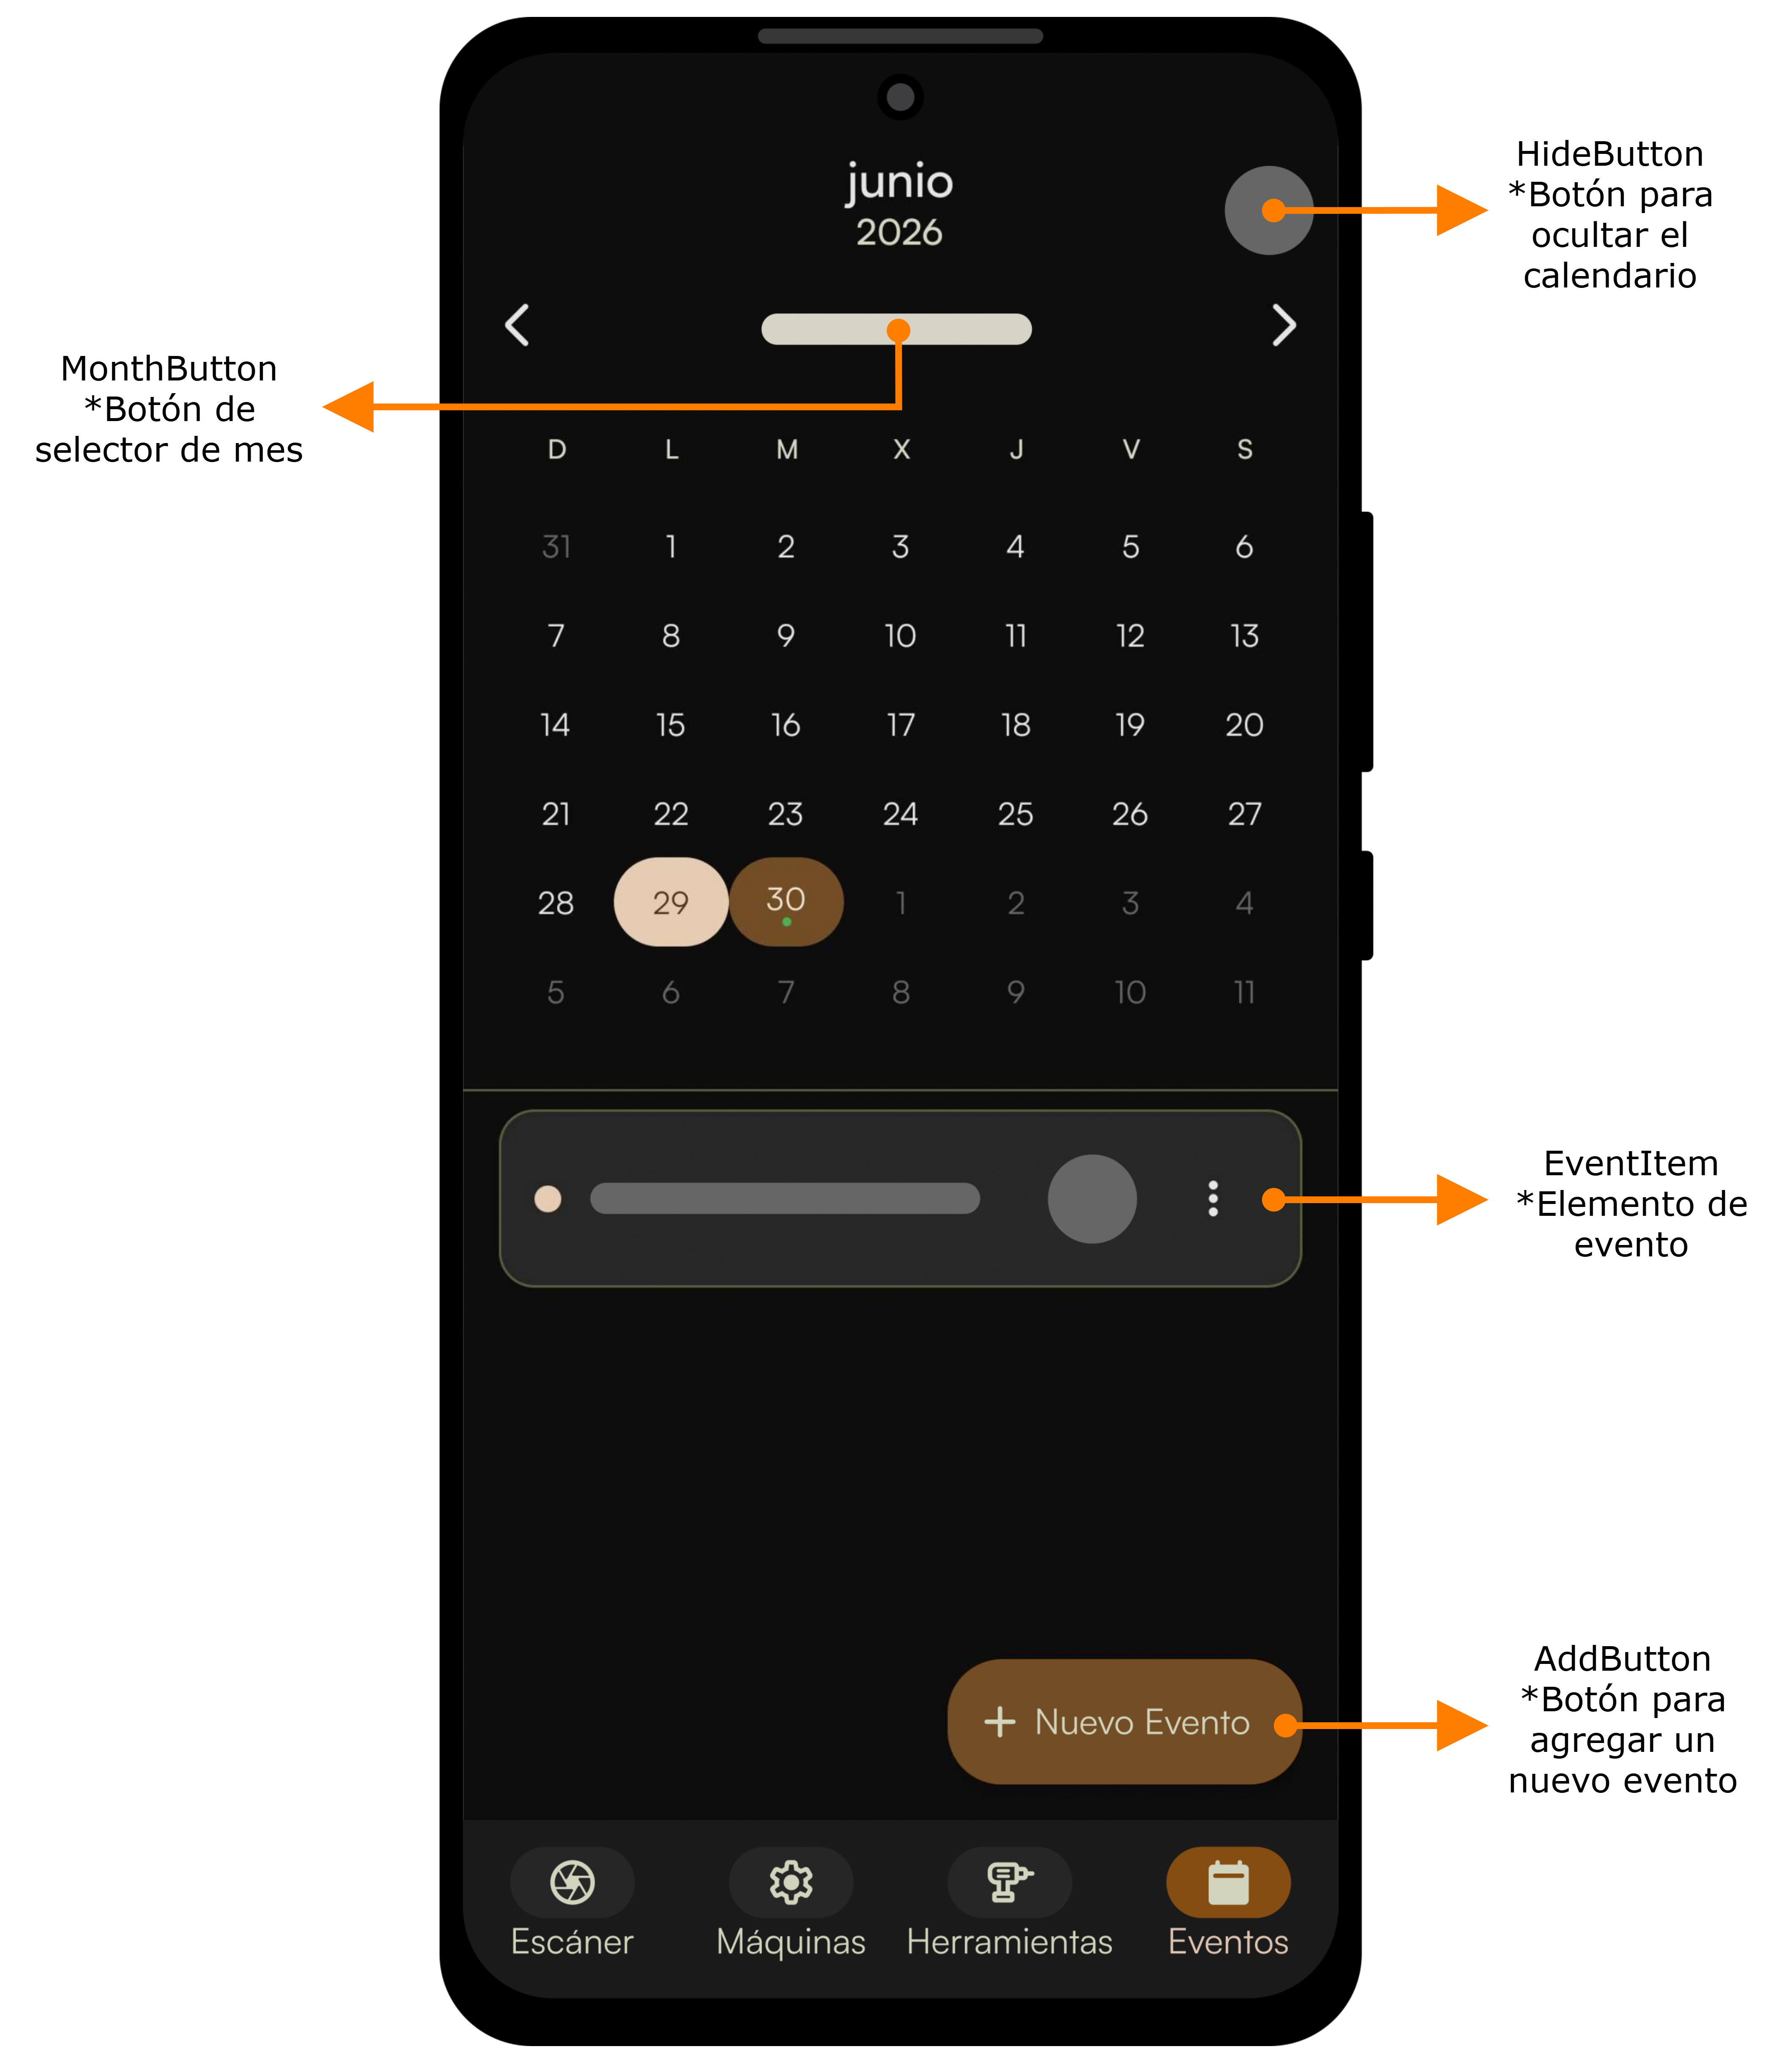
\includegraphics[height=12cm]{assets/figures/second_phase/screen/img_screen_events.png}
    \label{fig:screen_events}
\end{figure}

                La Figura \ref{fig:screen_events} presenta una interfaz orientada al seguimiento cronológico de los eventos, permitiendo consultar de forma rápida la información asociada a cada actividad registrada.

        \subsubsection{Diseño de las pantallas de información técnica}

            Las pantallas de consulta de información concentran los diferentes recursos asociados a cada máquina registrada en el sistema. Este grupo está conformado por las pantallas de especificaciones, documentación y actividades de mantenimiento. Aunque cada una presenta un contenido diferente, comparten una distribución similar de los elementos de interfaz, favoreciendo una experiencia de usuario consistente.

            \paragraph{La pantalla de especificaciones}

                concentra la información técnica correspondiente a la máquina seleccionada, permitiendo consultar sus principales características de manera organizada, incorporando una imagen principal del equipo cuando esta se encuentra disponible para facilitar su identificación.

                \begin{figure}[H]
    \caption{Pantalla de especificaciones}
    \centering
    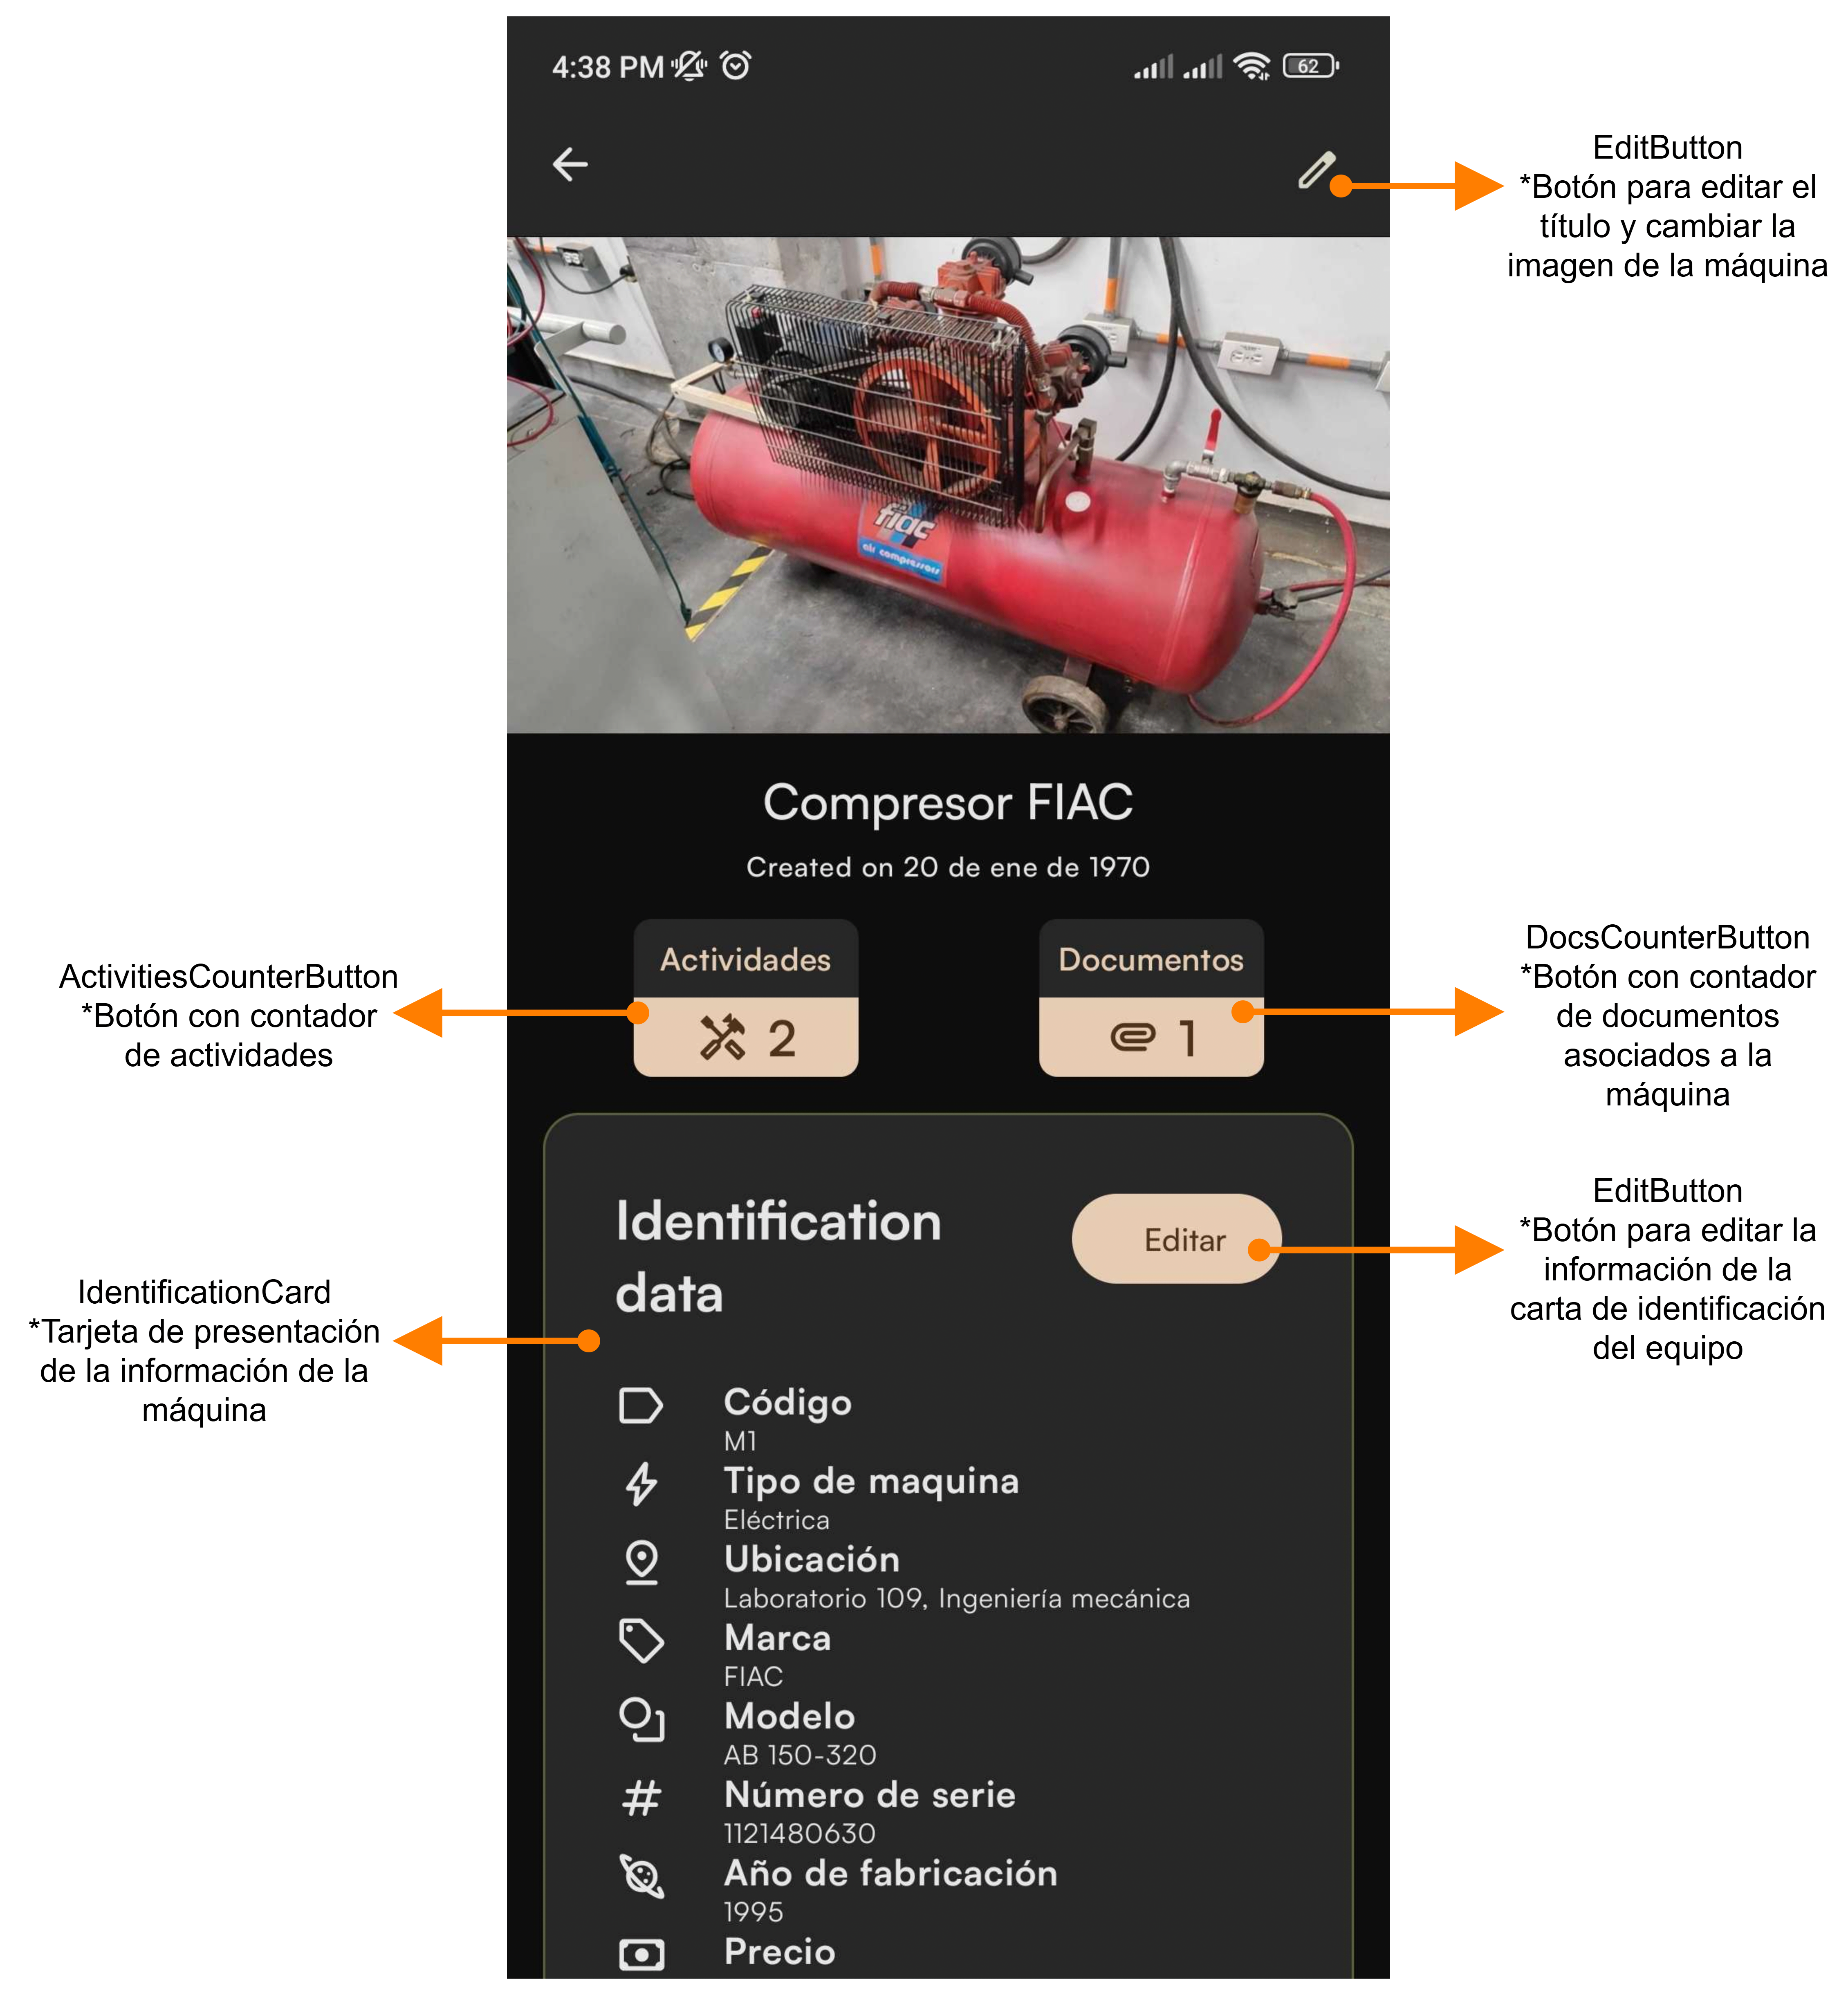
\includegraphics[height=12cm]{assets/figures/second_phase/secondary_screen/img_screen_specs.png}
    \label{fig:screen_specs}
\end{figure}

                Como se observa en la Figura \ref{fig:screen_specs}, la información se presenta mediante tarjetas temáticas presentes en los Apéndices \ref{apc:machine_cards} y \ref{apc:motor_cards}.

            \paragraph{La pantalla de documentación}

                permite consultar los documentos PDF asociados a una máquina específica, centralizando manuales, instructivos u otros archivos técnicos relevantes para el proceso de mantenimiento.

                \begin{figure}[H]
    \caption{Pantalla de documentos}
    \centering
    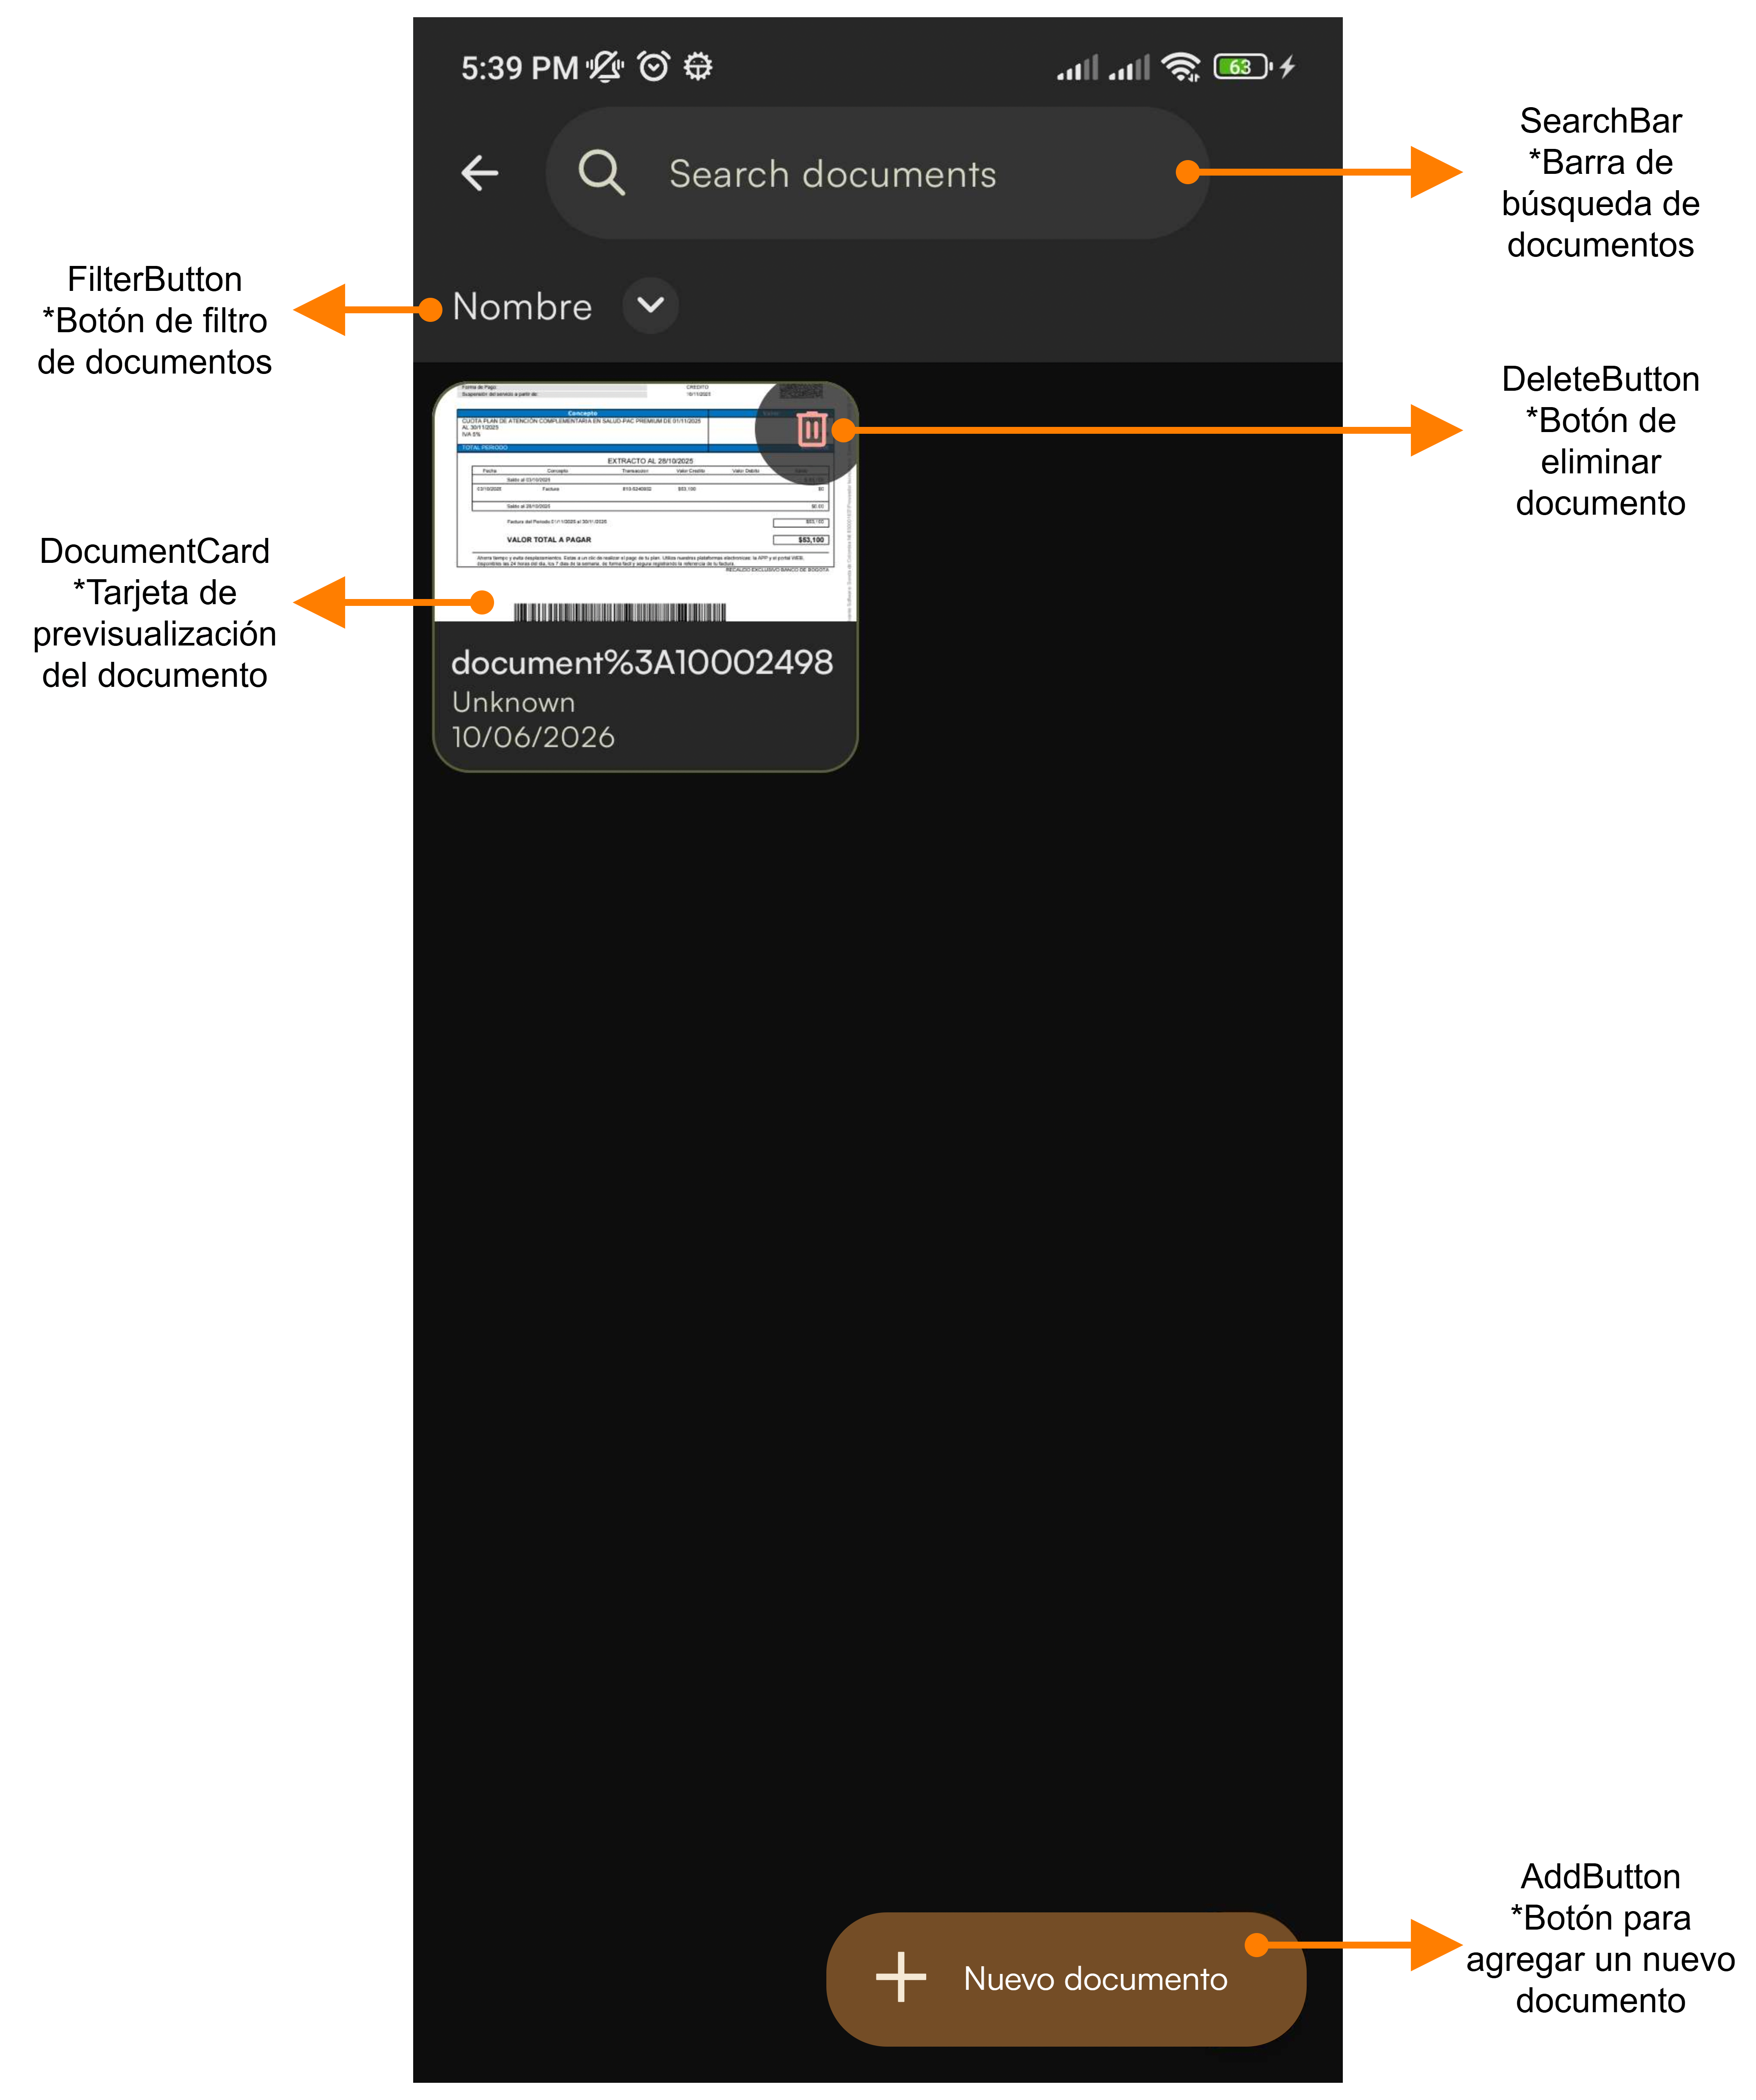
\includegraphics[height=12cm]{assets/figures/second_phase/secondary_screen/img_screen_documents.png}
    \label{fig:screen_documents}
\end{figure}

                Como se aprecia en la Figura \ref{fig:screen_documents}, los documentos se presentan en forma de malla, permitiendo acceder rápidamente a cada archivo para su consulta desde el propio dispositivo móvil.

            \paragraph{La pantalla de actividades de mantenimiento}

                reúne las diferentes actividades registradas para la máquina seleccionada, constituyendo el punto de acceso a los procedimientos de realidad aumentada.

                \begin{figure}[H]
    \caption{Pantalla de cronograma de eventos}
    \centering
    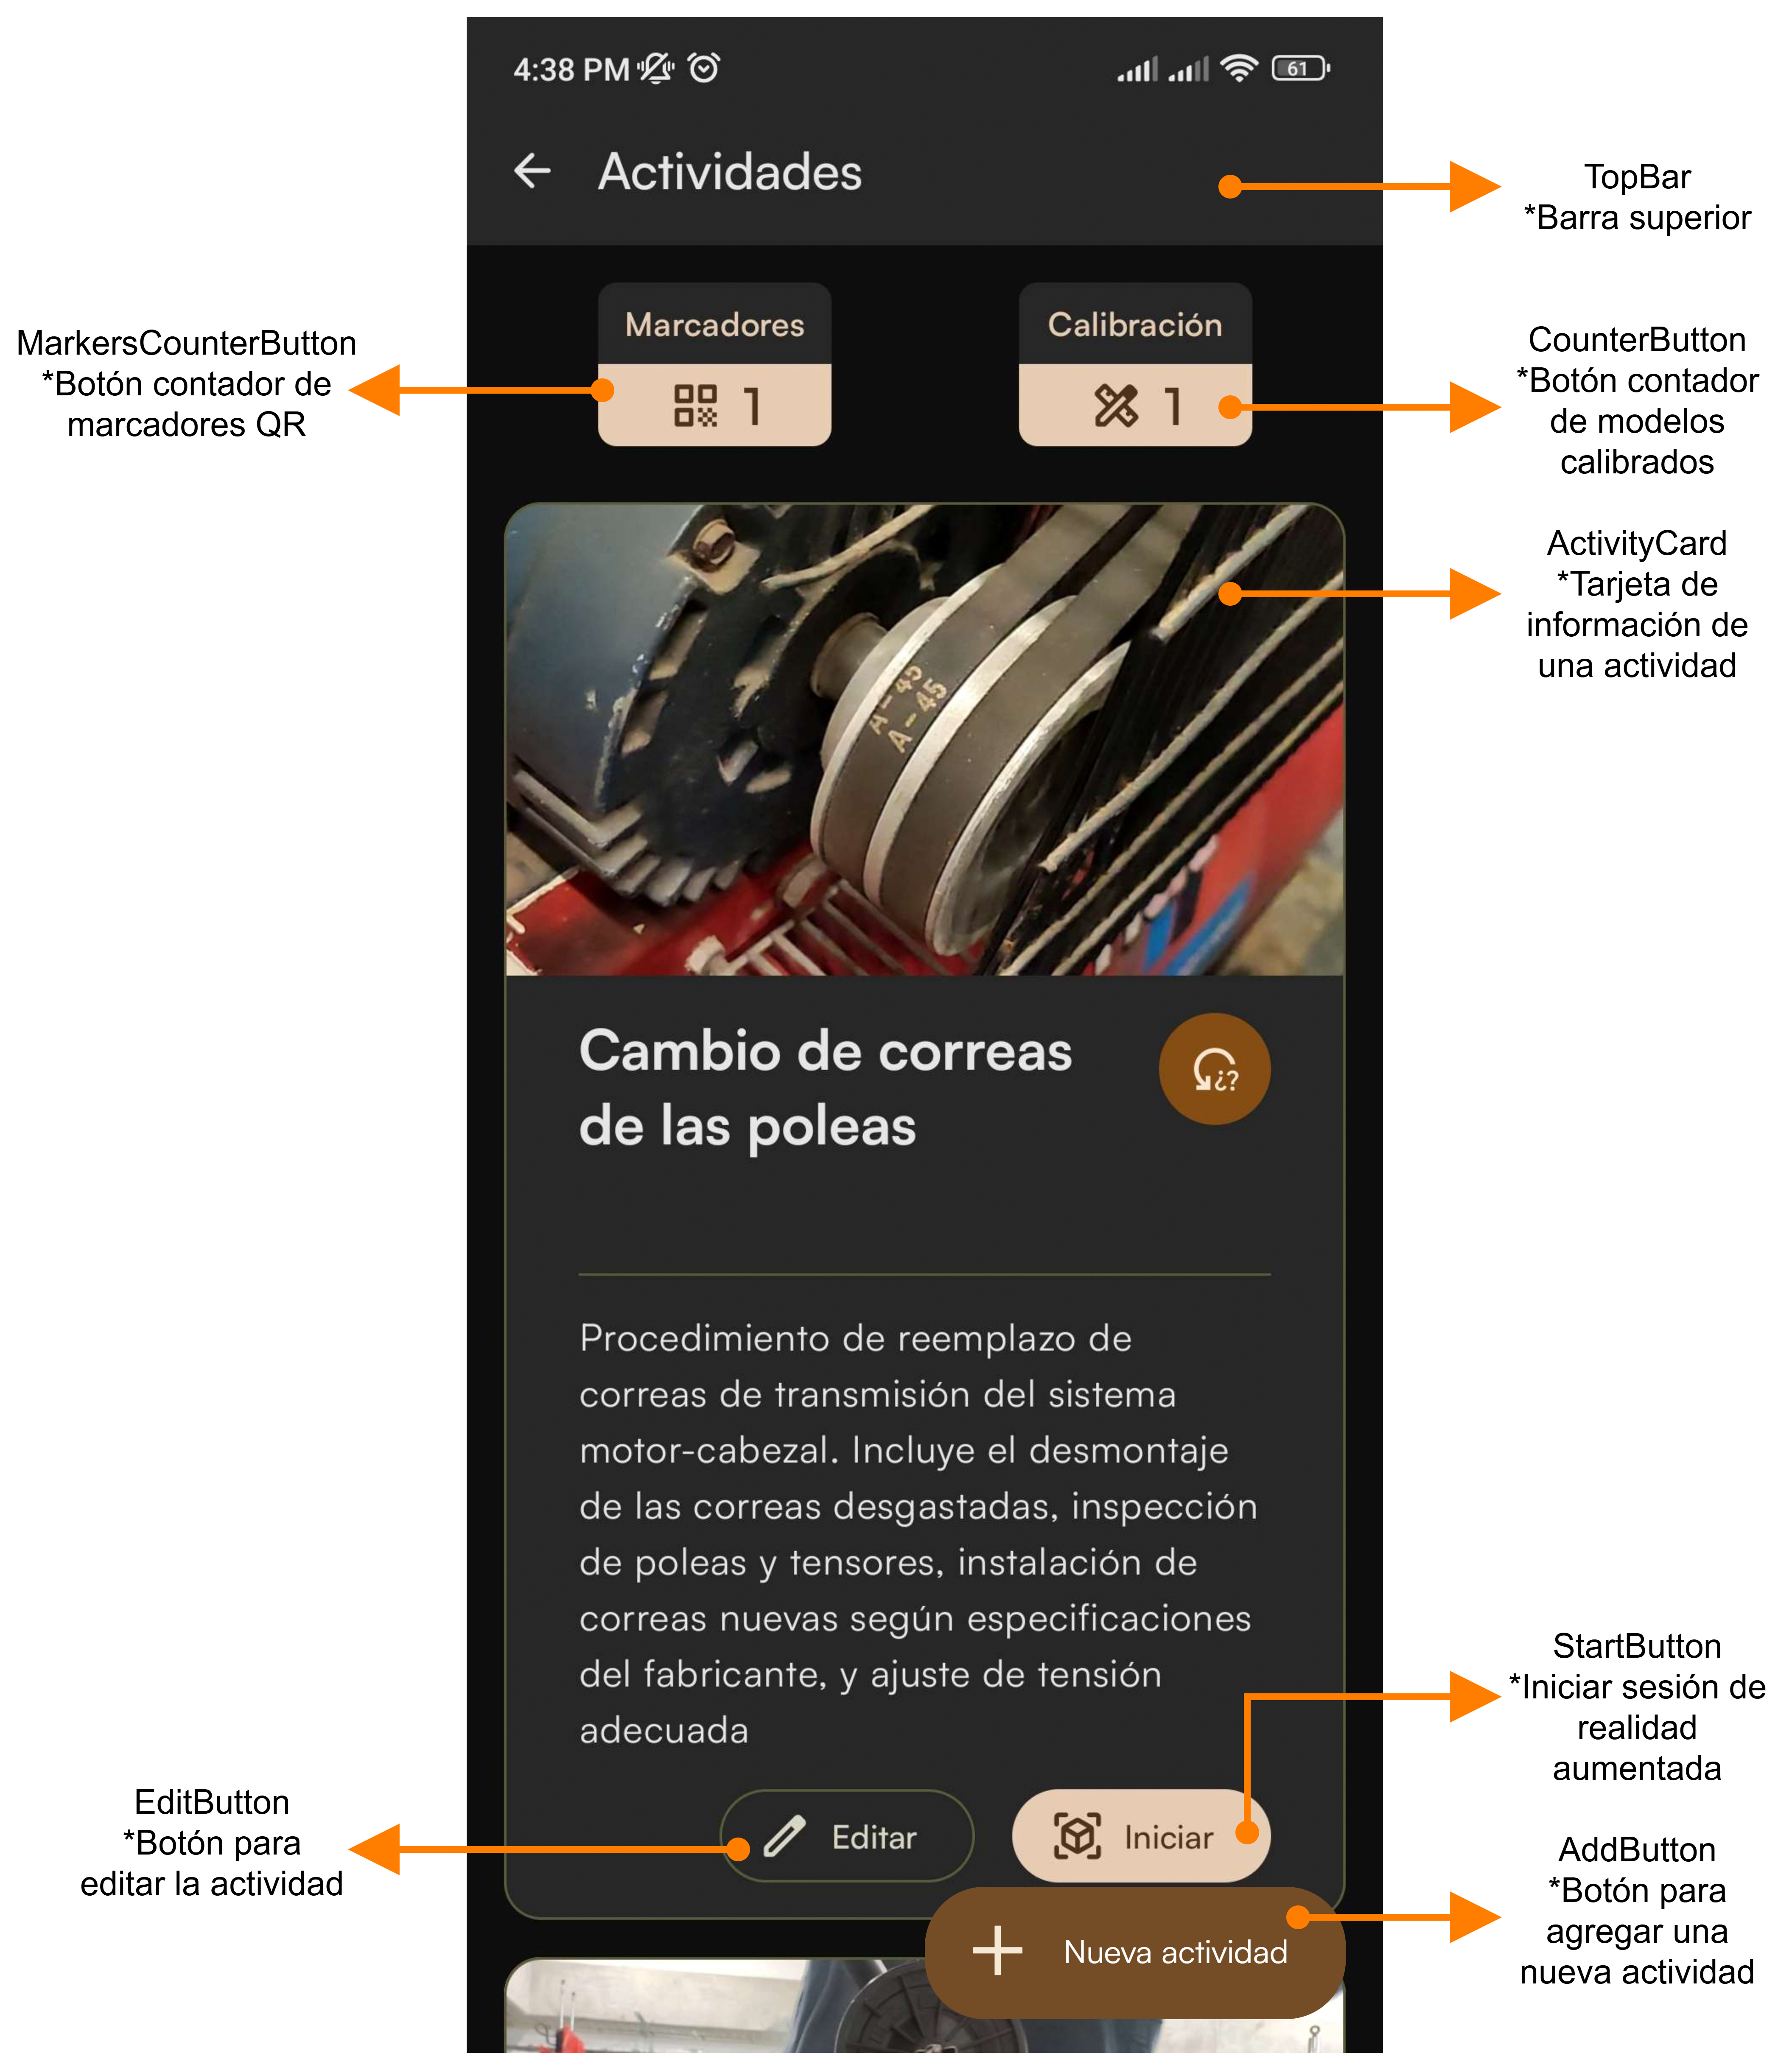
\includegraphics[height=12cm]{assets/figures/second_phase/secondary_screen/img_screen_activities.png}
    \label{fig:screen_activities}
\end{figure}

                Como se muestra en la Figura \ref{fig:screen_activities}, las actividades se presentan en un listado organizado que facilita su consulta y selección. Desde esta pantalla el usuario puede identificar el procedimiento de mantenimiento que desea ejecutar antes de iniciar la correspondiente sesión de realidad aumentada.

        \subsubsection{Diseño de las pantallas de configuración previa de realidad aumentada}

            La configuración de las escenas de realidad aumentada se realiza mediante un flujo compuesto por tres pantallas principales, las cuales permiten preparar todos los elementos necesarios antes de ejecutar una sesión de mantenimiento asistida. Este flujo comprende la creación de marcadores, la calibración de los modelos tridimensionales y la definición de las actividades de mantenimiento que posteriormente serán visualizadas durante la experiencia de realidad aumentada.

            \paragraph{Pantalla de marcadores}

                El proceso de configuración de una escena de realidad aumentada inicia con la creación de los marcadores que servirán como referencia espacial para cada máquina. Para ello, el aplicativo incorpora la pantalla de marcadores, la cual permite generar y administrar los códigos QR asociados a los diferentes equipos.

                \begin{figure}[H]
    \caption{Pantalla de marcadores}
    \centering
    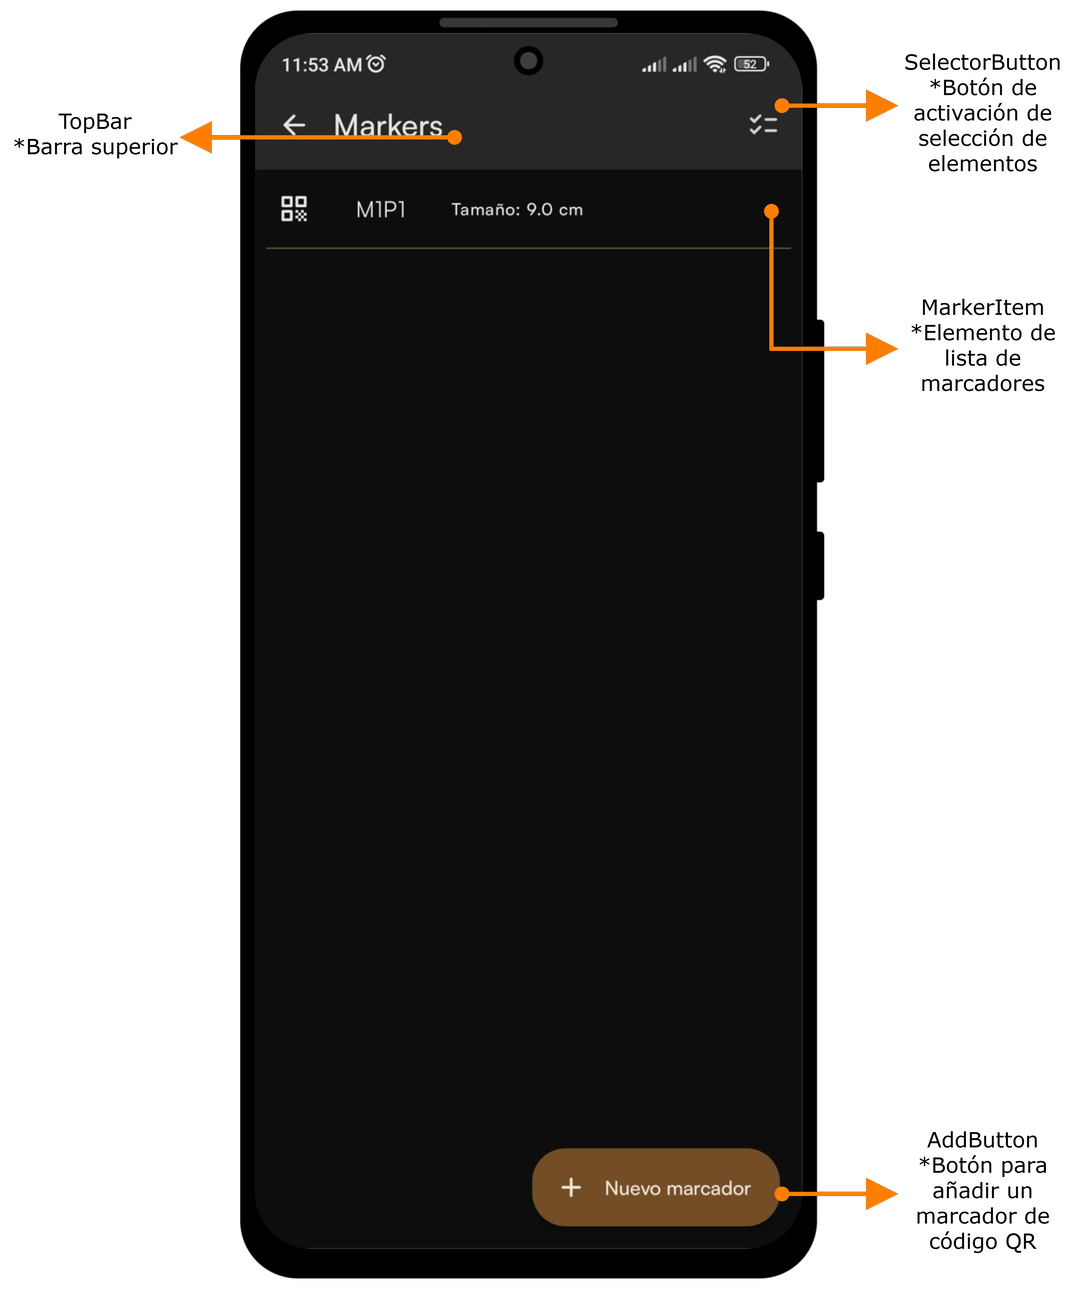
\includegraphics[height=12cm]{assets/figures/second_phase/secondary_screen/img_screen_markers.png}
    \label{fig:screen_markers}
\end{figure}

                Como se observa en la Figura \ref{fig:screen_markers}, la interfaz presenta el listado de marcadores registrados y proporciona las opciones necesarias para crear nuevos marcadores o administrar los existentes. Además, incorpora una función para exportarlos conjuntamente en un único archivo PDF, facilitando su impresión o laminación para su utilización en el entorno real.

                Una vez impresos, estos marcadores actúan como referencia para el posicionamiento y seguimiento de los modelos tridimensionales durante las sesiones de realidad aumentada, constituyendo el punto de partida para el proceso de calibración descrito a continuación.

            \paragraph{Pantalla de calibración de modelos 3D}

                Después de crear los marcadores, el usuario continúa con la calibración de los modelos tridimensionales mediante la pantalla de calibración, donde se define la posición y orientación que tendrán los modelos con respecto al marcador físico seleccionado.

                \begin{figure}[H]
    \caption{Pantalla de calibración de modelos 3D}
    \centering
    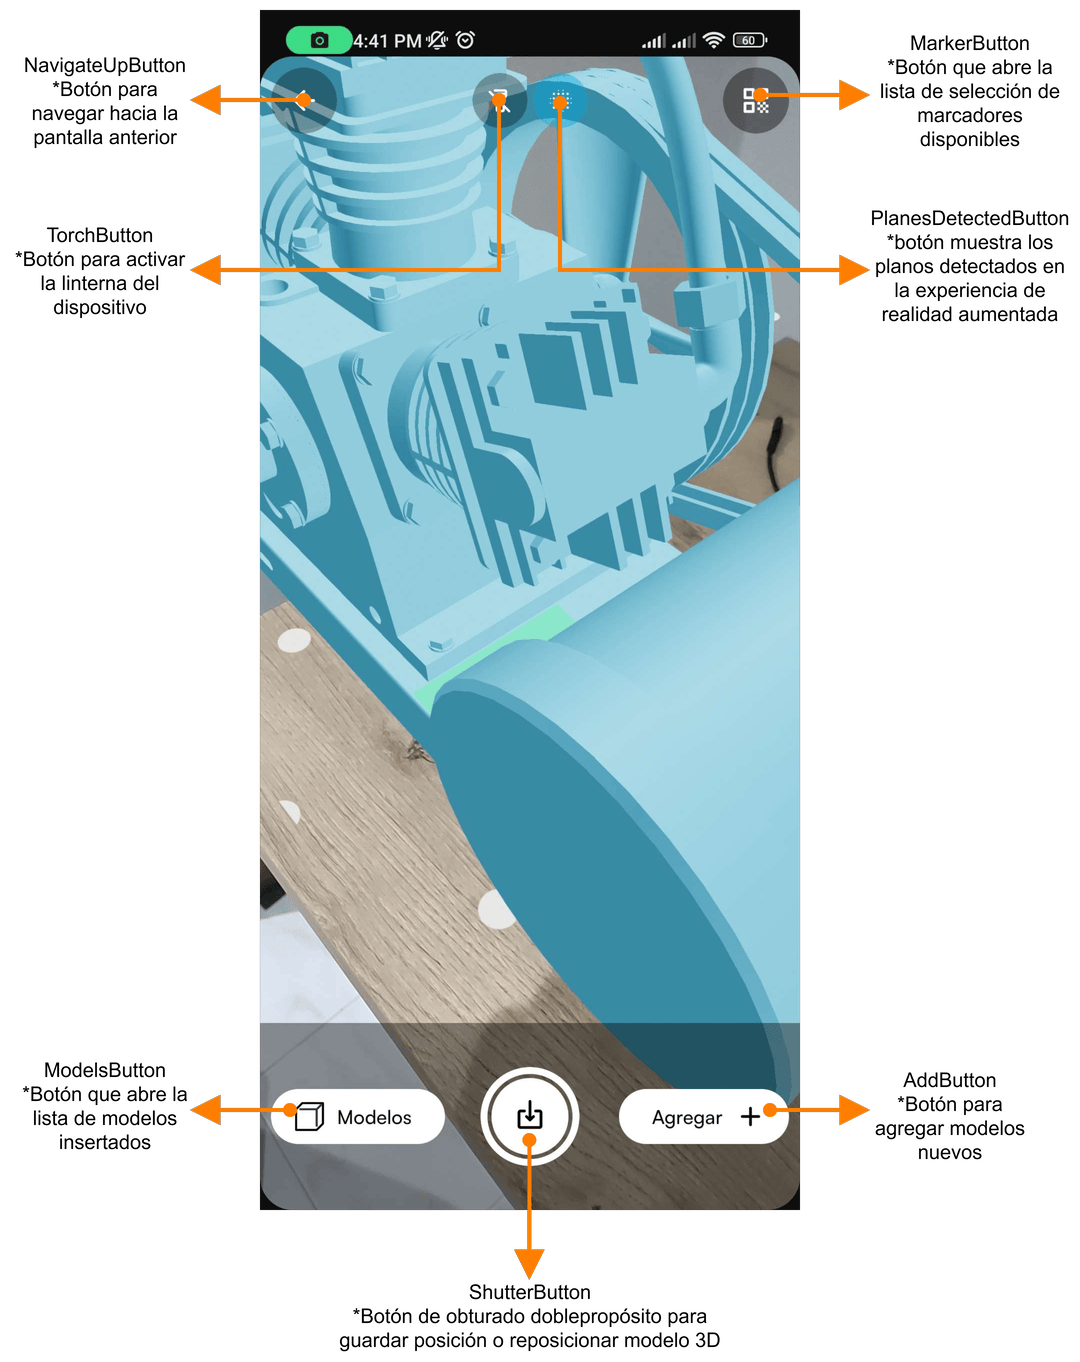
\includegraphics[height=12cm]{assets/figures/second_phase/secondary_screen/img_screen_calibration.png}
    \label{fig:screen_calibration}
\end{figure}

                Como se aprecia en la Figura \ref{fig:screen_calibration}, la interfaz incorpora un selector de marcadores, herramientas para la inserción de modelos en formato \textbf{.glb}, un menú destinado al reposicionamiento de los modelos 3D y un botón de obturador con doble funcionalidad. Una pulsación simple permite guardar la posición actual de los modelos, mientras que al mantenerlo presionado se reposicionan tomando como referencia el marcador activo de la escena.

                Antes de habilitar las funciones de edición, el usuario debe escanear el marcador físico mediante la cámara del dispositivo. Cuando el reconocimiento se realiza correctamente, la aplicación proyecta un nodo de plano virtual sobre el marcador para indicar el estado del seguimiento visto en la Figura \ref{fig:node_plane}.

                Una vez detectado el marcador, se habilitan las herramientas de edición. El usuario puede insertar modelos tridimensionales y ajustar su posición y orientación respecto al marcador seleccionado, estableciendo la configuración espacial que será utilizada posteriormente durante la ejecución de la experiencia de realidad aumentada.

                Los controles de reposicionamiento de modelos, ilustrados en la Figura \ref{fig:calibration_controls}, se encuentran en un panel inferior expandible que organiza cinco categorías de botones. La primera permite seleccionar el modo de transformación, ya sea posición u orientación; la segunda define la unidad de medida correspondiente al modo seleccionado; la tercera permite restaurar los valores predeterminados; la cuarta está compuesta por un conjunto de ruedas o deslizadores con una resolución máxima de una unidad de medida; y la quinta consiste en un botón para eliminar el modelo seleccionado. Al interactuar con los deslizadores, se activan los nodos de eje ilustrados en la Figura \ref{fig:node_axes}, los cuales proporcionan al usuario una guía visual sobre la dirección en la que puede desplazarse el modelo 3D.

                \begin{figure}[H]
    \caption{Controles para calibración de modelos 3D}
    \centering
    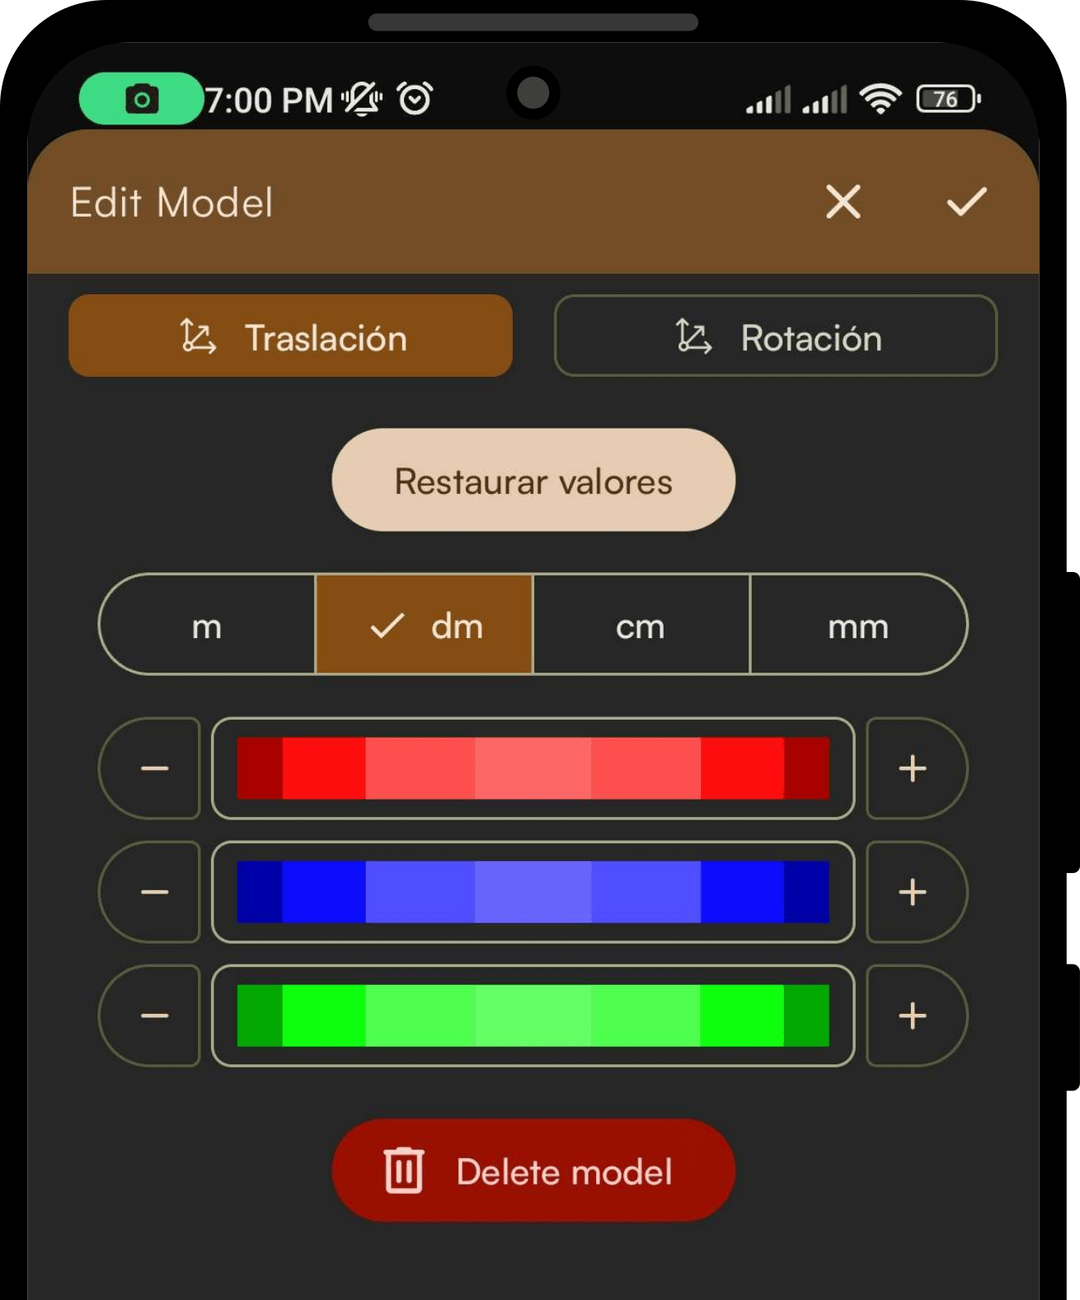
\includegraphics[width=0.4\textwidth]{assets/figures/second_phase/controls/img_calibration_controls.png}
    \label{fig:calibration_controls}
\end{figure}
\fixvspace{0}

            \paragraph{Pantalla de editor de actividades de mantenimiento}

                Una vez finalizada la calibración de los modelos, el usuario procede a definir las actividades de mantenimiento mediante la pantalla del editor de actividades. A diferencia de las interfaces de realidad aumentada, esta pantalla no incorpora una vista de cámara, ya que está orientada exclusivamente a la creación y edición de las animaciones que compondrán cada procedimiento de mantenimiento.

                \begin{figure}[H]
    \caption{Pantalla de editor de actividades de mantenimiento}
    \centering
    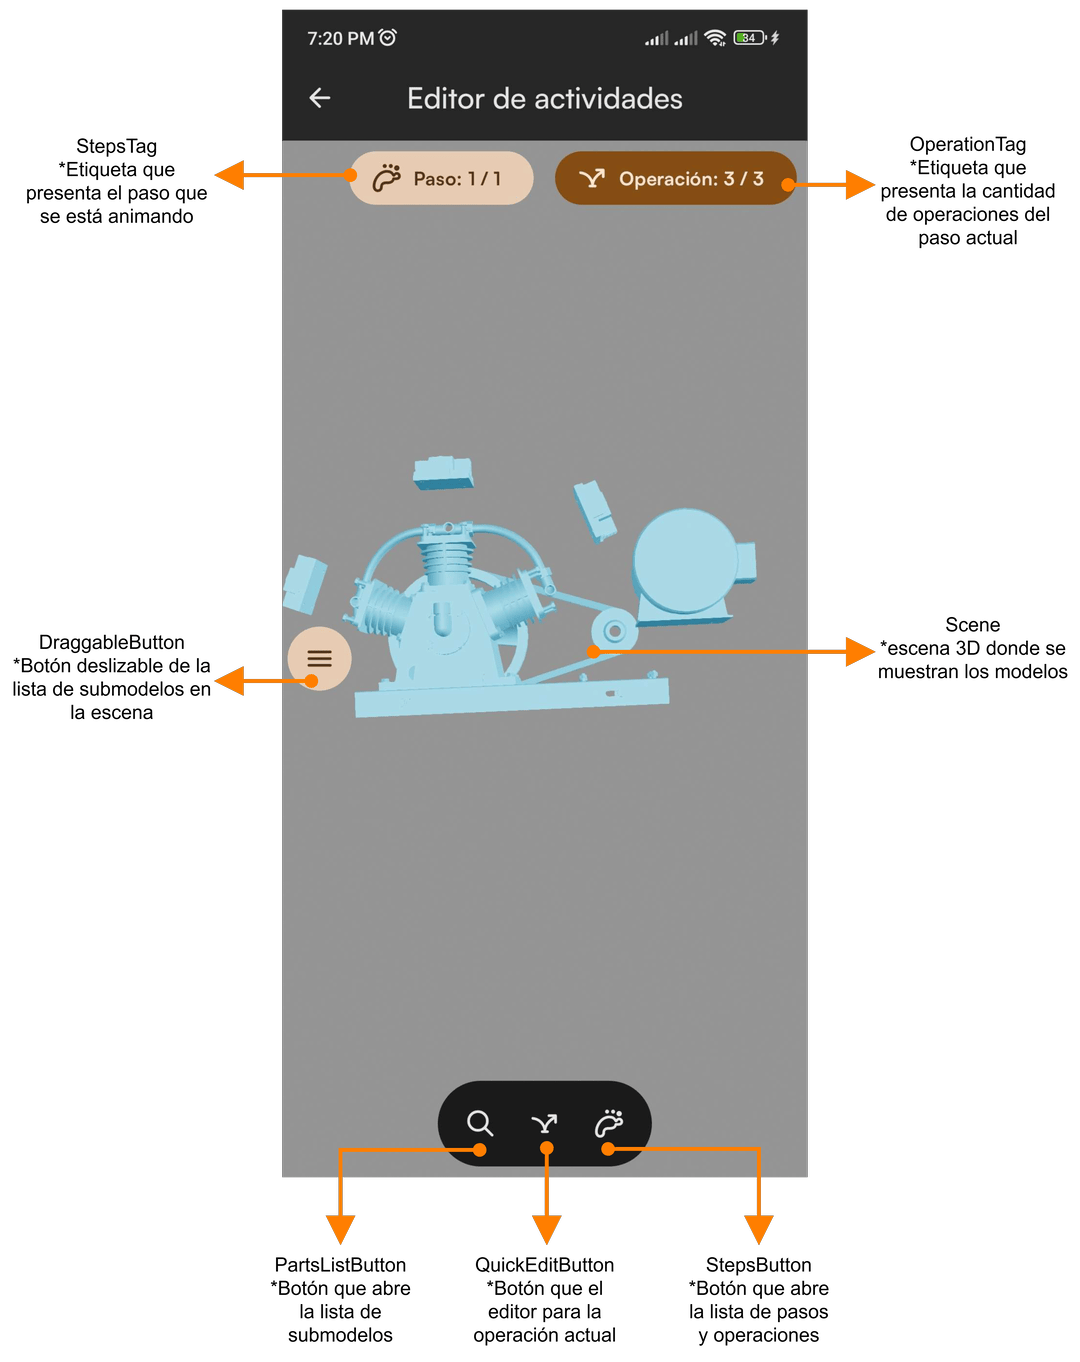
\includegraphics[height=12cm]{assets/figures/second_phase/secondary_screen/img_screen_editor.png}
    \label{fig:screen_editor}
\end{figure}

                Como se observa en la Figura \ref{fig:screen_editor}, la interfaz integra diferentes paneles destinados a facilitar la edición de las actividades. Entre ellos se encuentran el listado de submodelos (Figura \ref{fig:screen_editor_parts_list}), que permite mostrar u ocultar las distintas piezas del modelo tridimensional, y el editor de pasos y operaciones (Figura \ref{fig:screen_editor_steps_list}), donde se construye la secuencia completa de mantenimiento.

                \begin{figure}[H]
    \caption{Panel de listado de submodelos 3D}
    \centering
    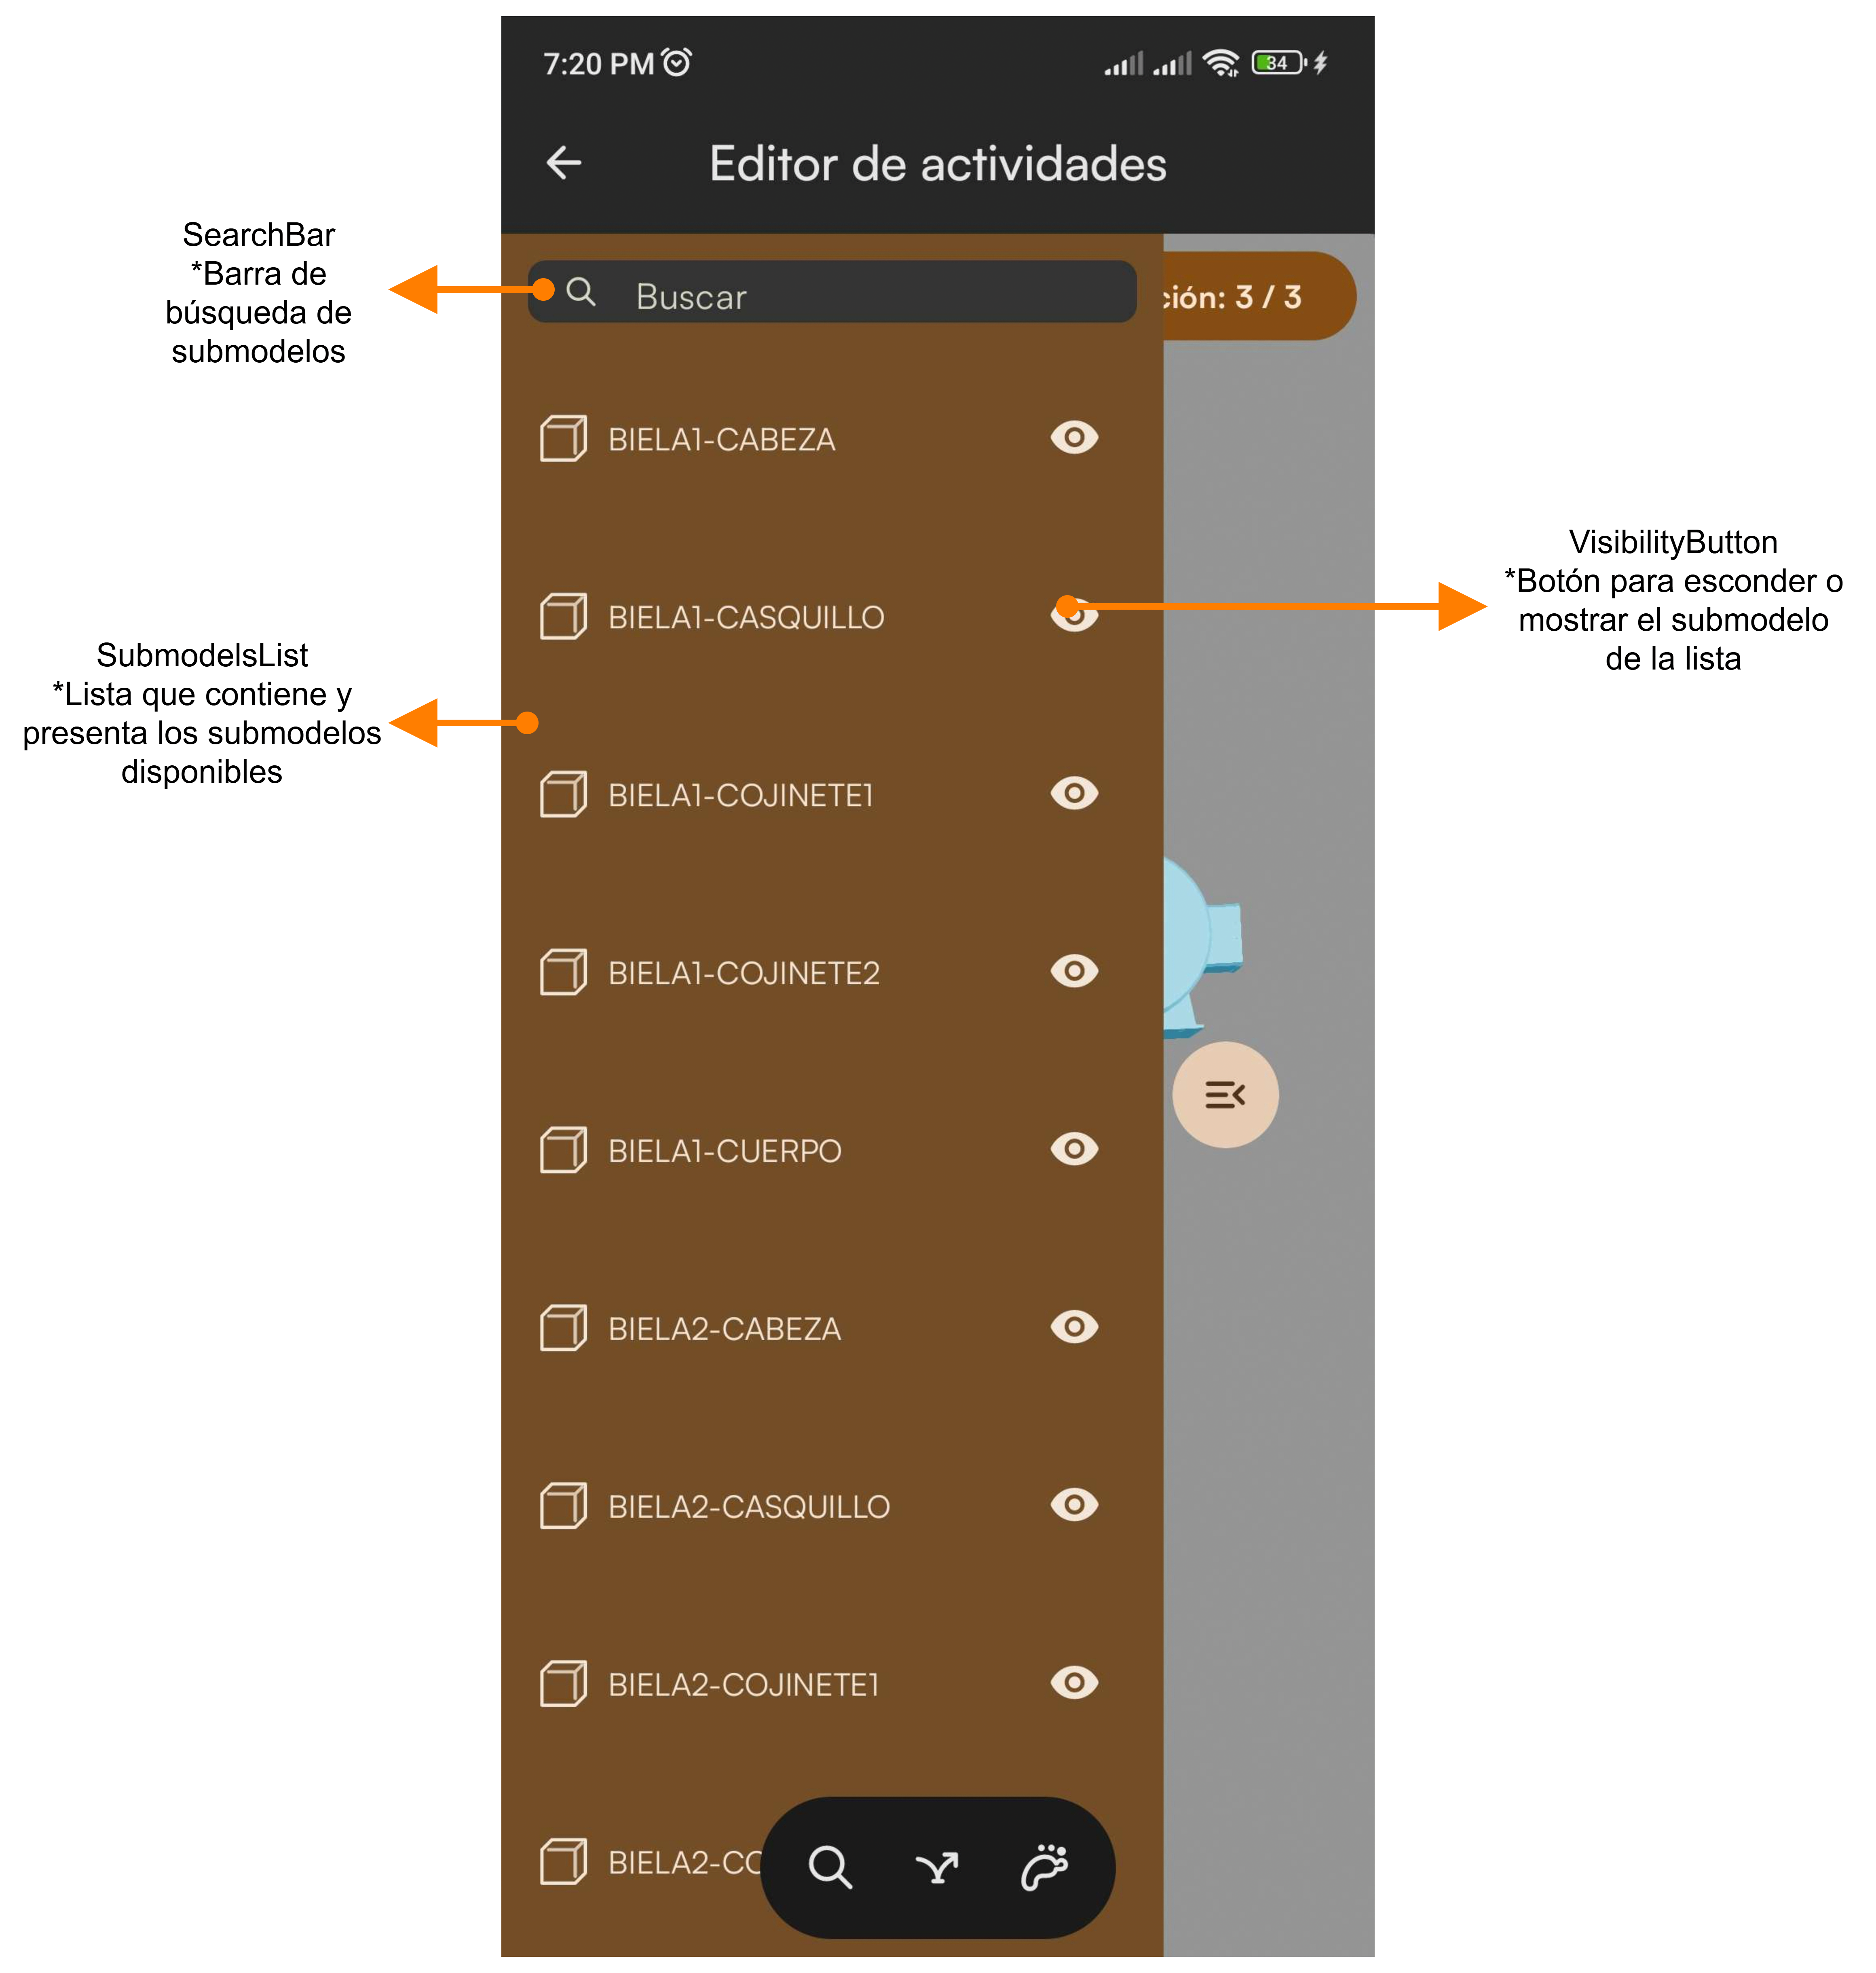
\includegraphics[height=12cm]{assets/figures/second_phase/secondary_screen/img_screen_editor_parts_list.png}
    \label{fig:screen_editor_parts_list}
\end{figure}

                \begin{figure}[H]
    \caption{Panel de listado de pasos y operaciones}
    \centering
    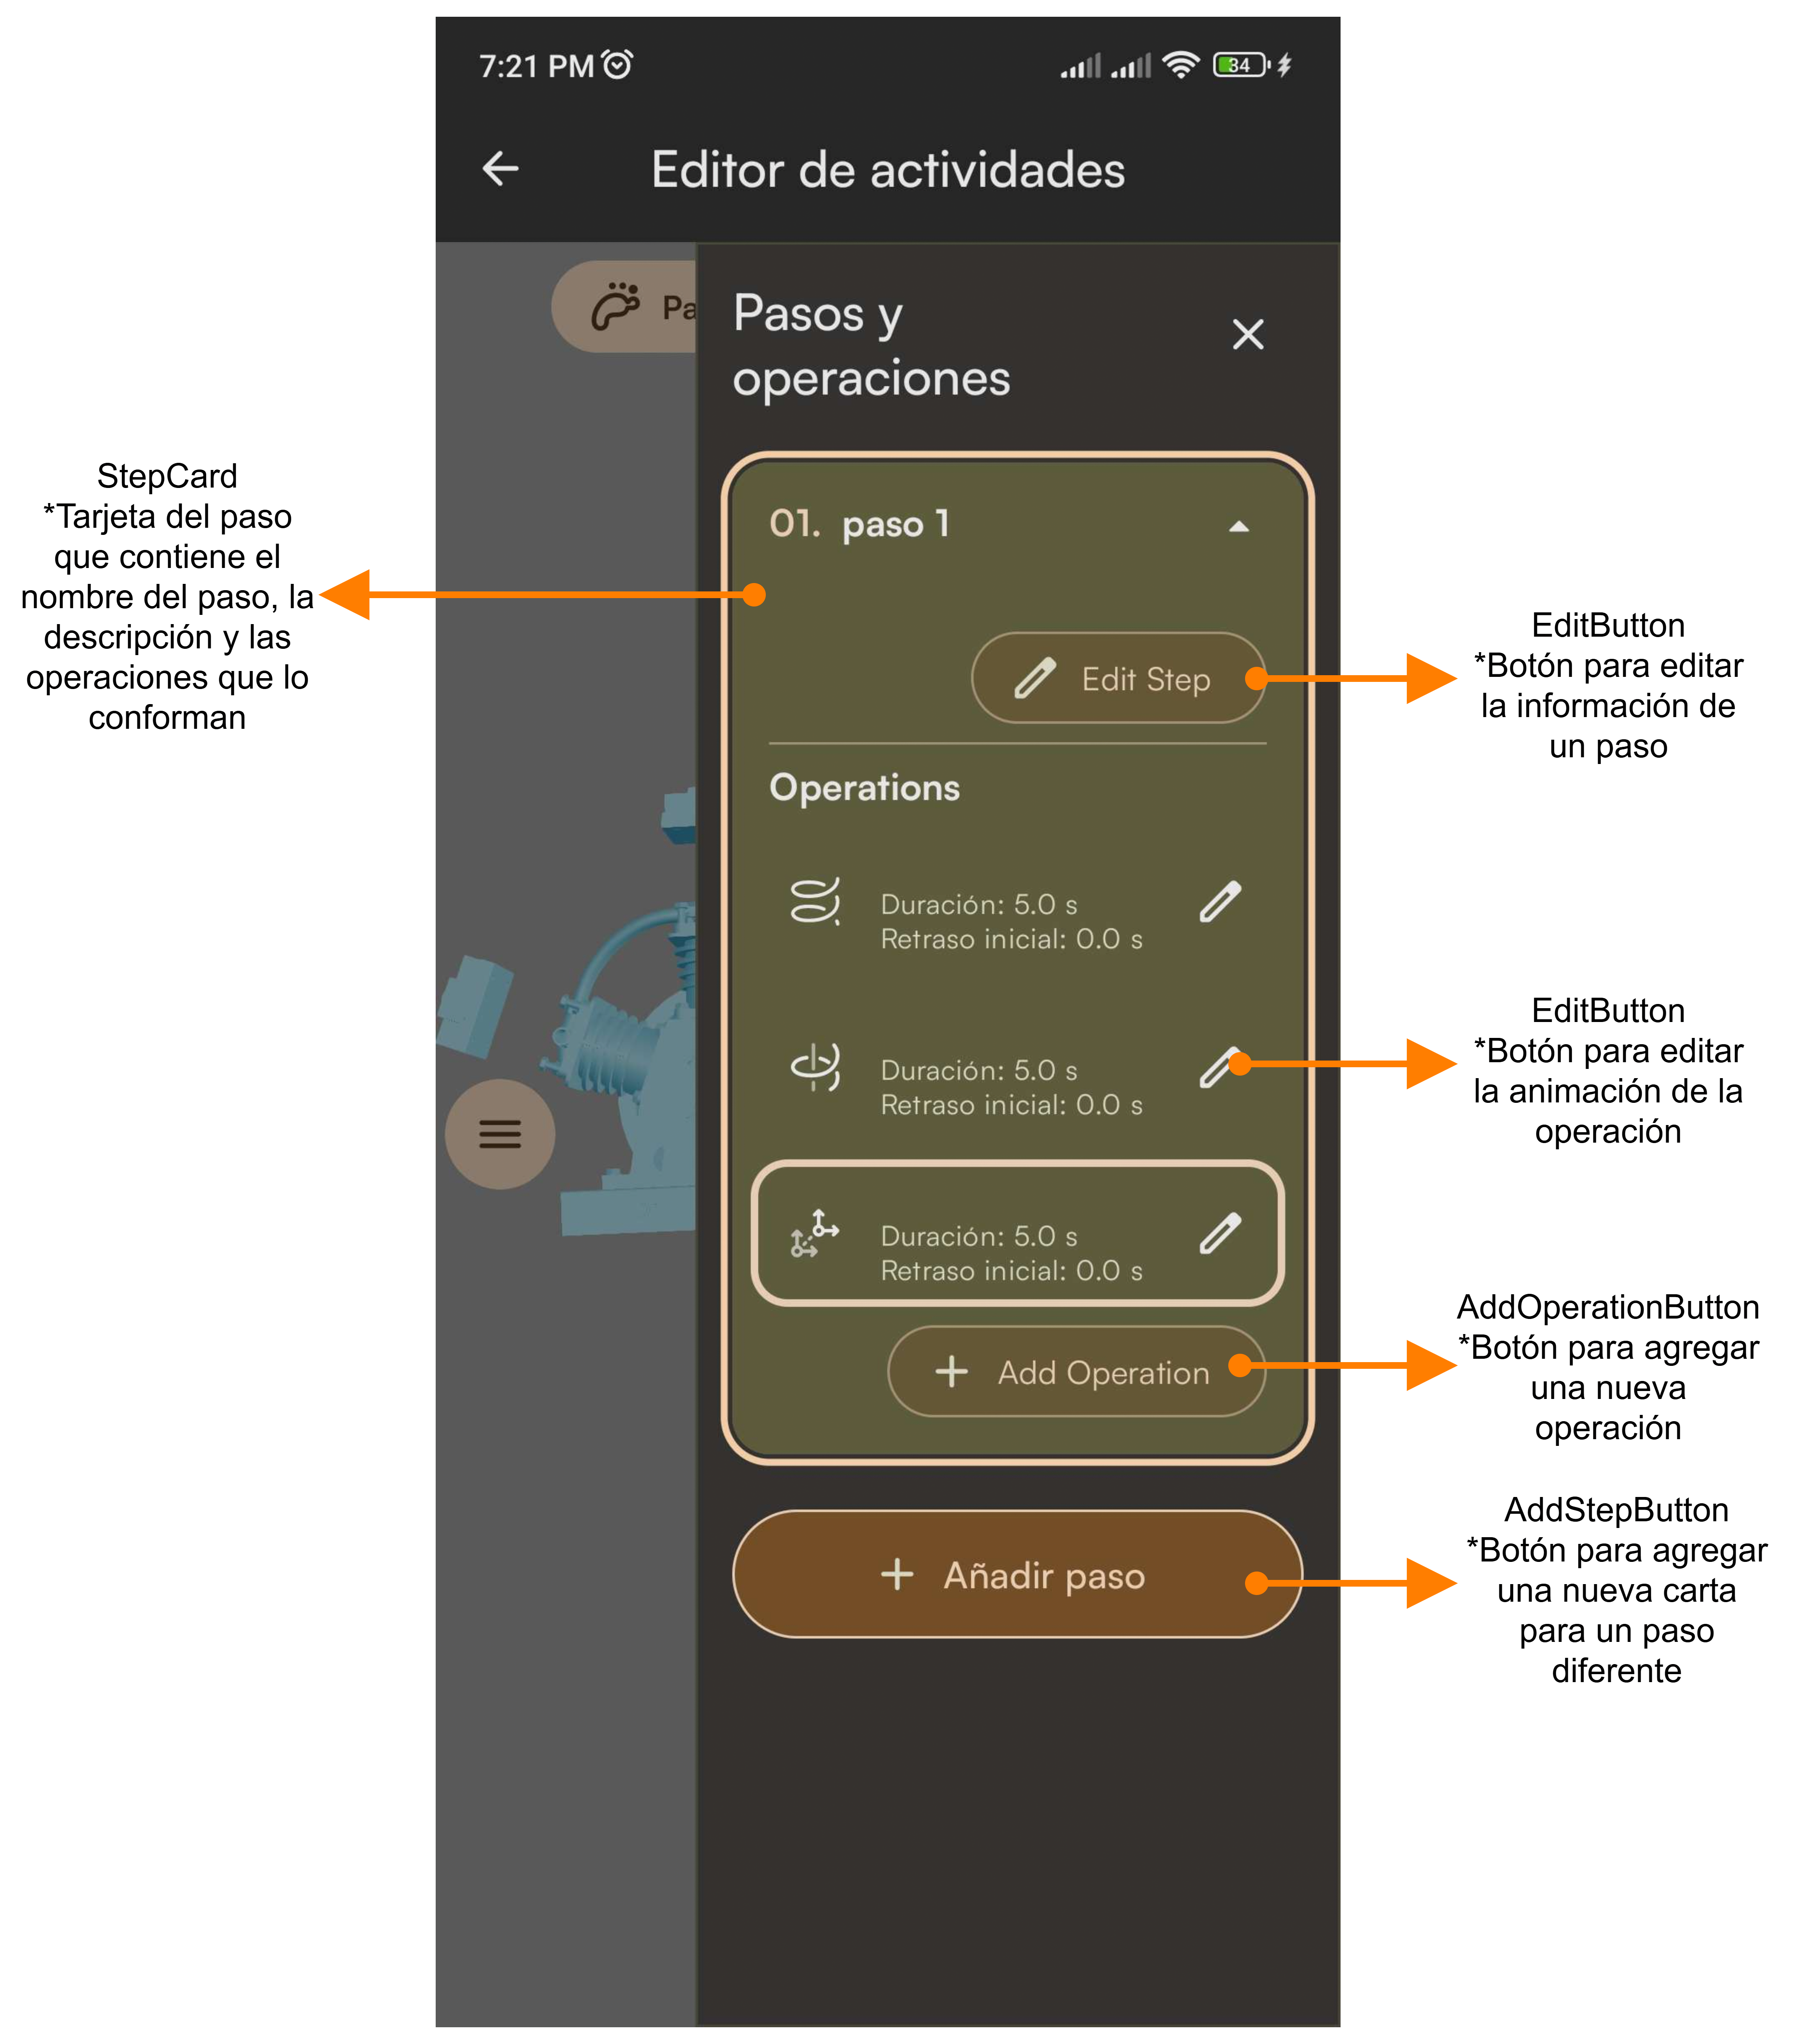
\includegraphics[height=12cm]{assets/figures/second_phase/secondary_screen/img_screen_editor_steps_list.png}
    \label{fig:screen_editor_steps_list}
\end{figure}

                Cada actividad se organiza en una serie de pasos, los cuales pueden contener una o varias operaciones encargadas de definir las animaciones de los submodelos seleccionados. Para ello el usuario deberá primero crear los pasos mediante el dialogo mostrado en la Figura \ref{fig:steps_dialog}, que habilitará la creación de operaciones que incorpora un panel inferior expandible, ilustrado en la Figura \ref{fig:operation_controls}, donde se seleccionará cuales submodelos serán animados de forma conjunta mediante su tipo de operacion: punto a punto, cilíndrica, junta y tornillo, cada una diseñada para representar diferentes comportamientos mecánicos.

                \begin{figure}[H]
    \caption{Diálogo de creación y edición de pasos}
    \centering
    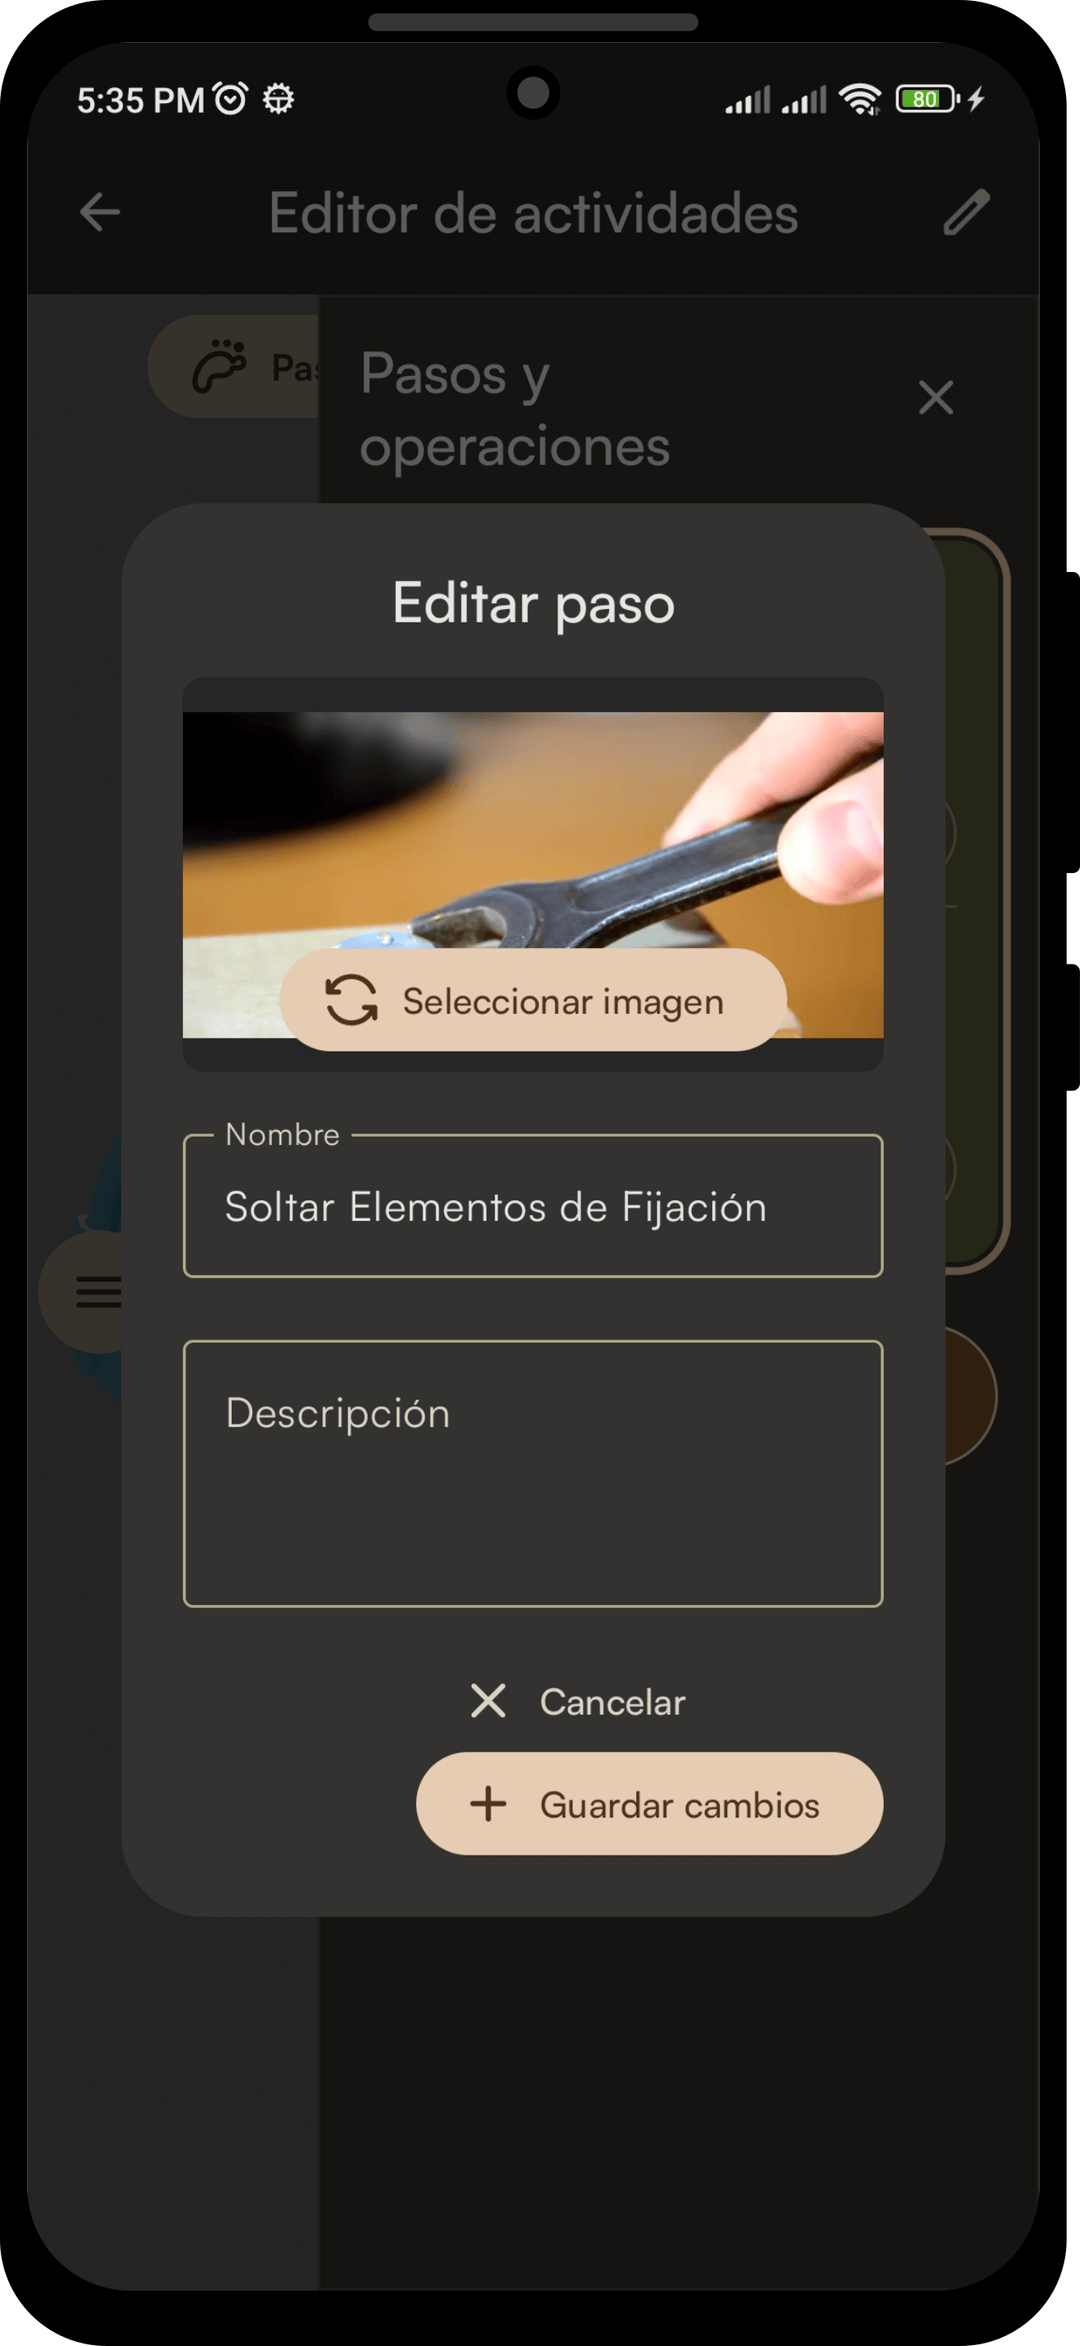
\includegraphics[width=0.4\textwidth]{assets/figures/second_phase/controls/img_steps_dialog.png}
    \label{fig:steps_dialog}
\end{figure}
\fixvspace{0}

                \begin{figure}[H]
    \caption{Controles para calibración de modelos 3D}
    \centering
    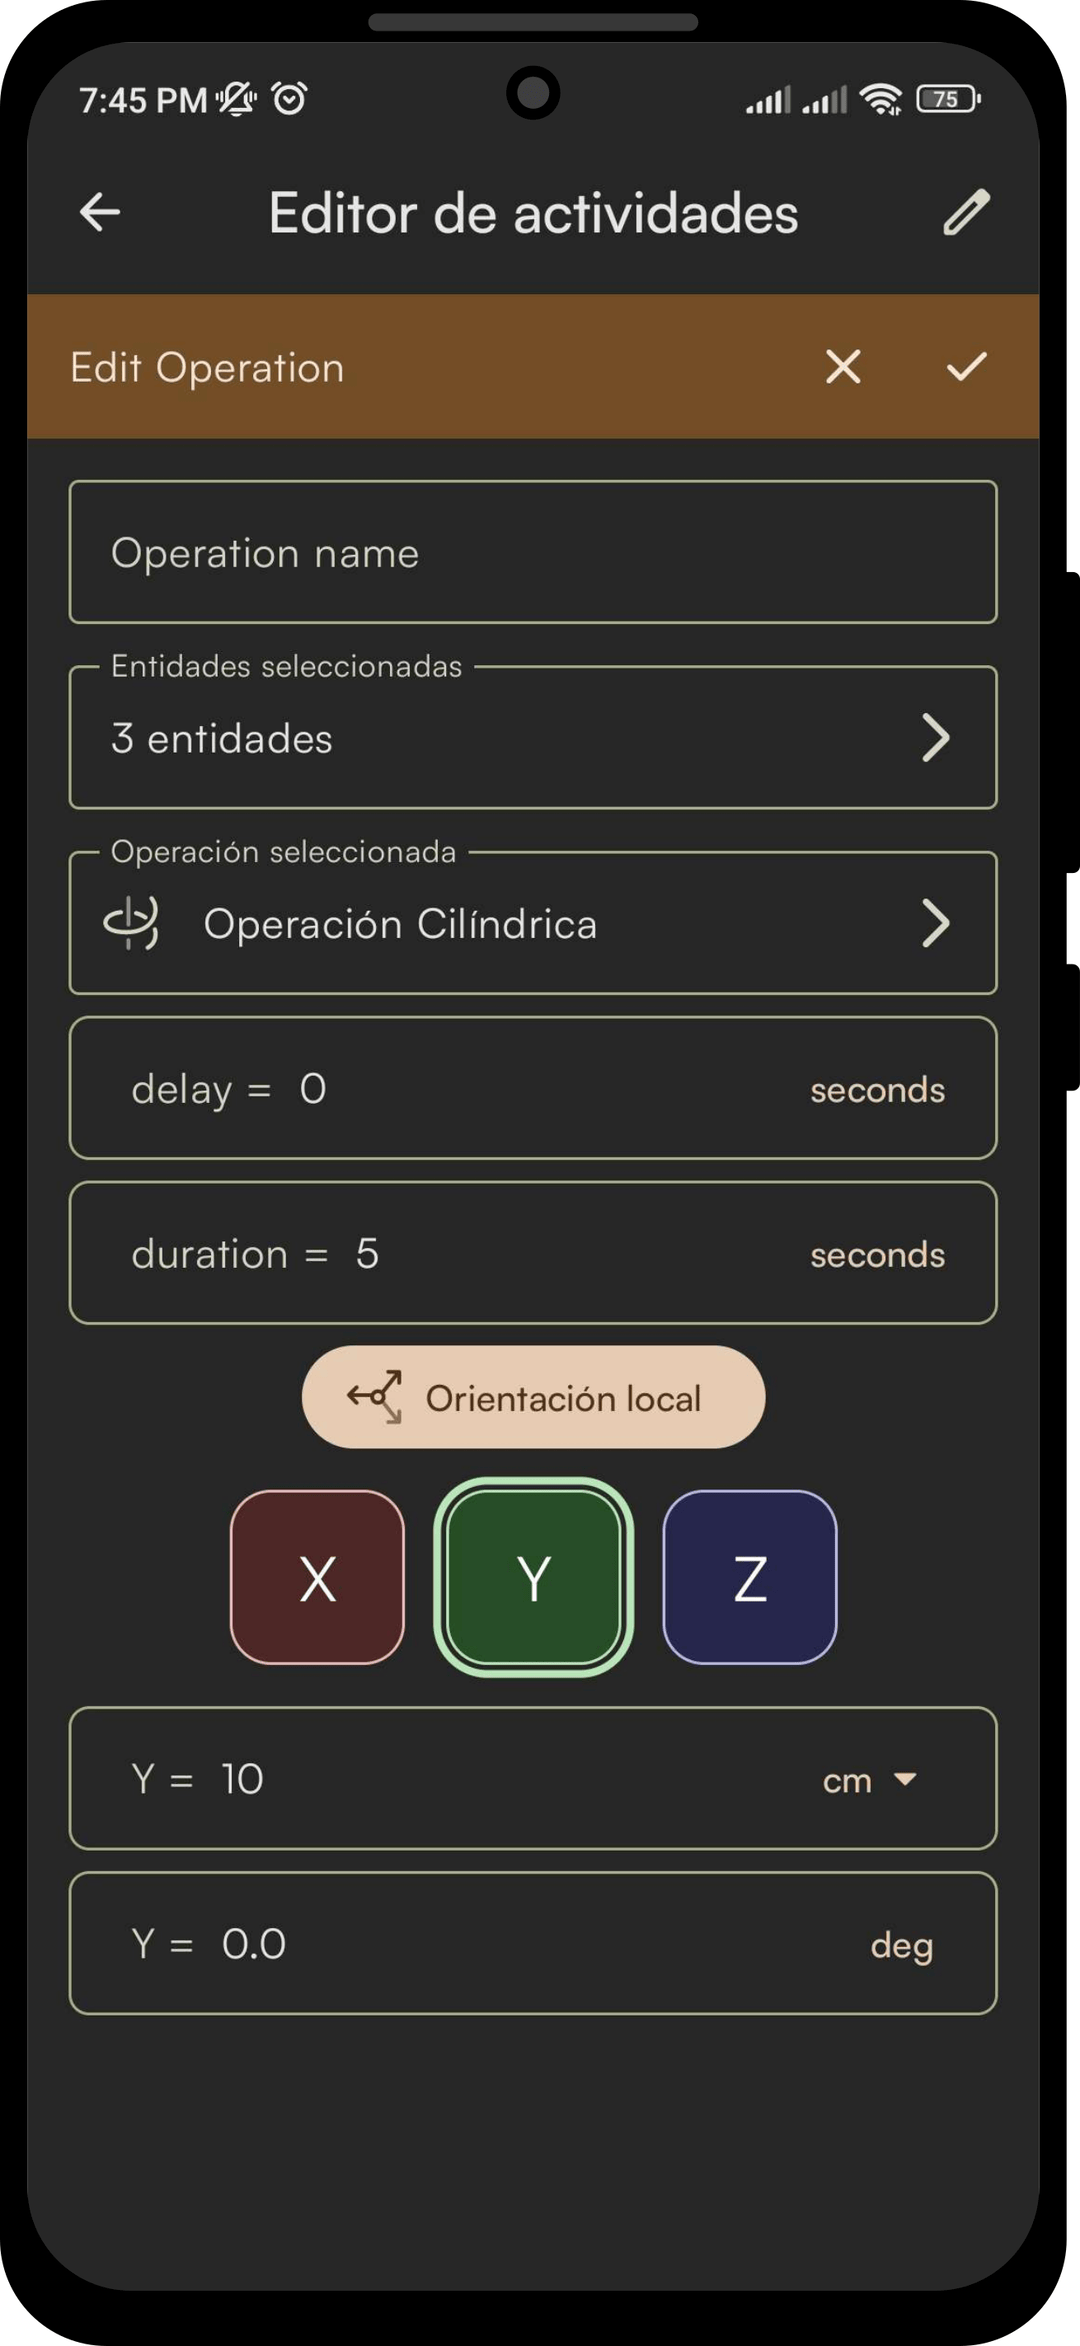
\includegraphics[width=0.4\textwidth]{assets/figures/second_phase/controls/img_operation_controls.png}
    \label{fig:operation_controls}
\end{figure}
\fixvspace{0}

                La Tabla \ref{tab:operations} resume las características de cada una de las operaciones, indicando los grados de libertad que implementan y una descripción general de su comportamiento durante la construcción de las animaciones.

                \begin{ThreePartTable}

    \renewcommand\TPTminimum{\textwidth}

    \setlength\LTleft{0pt}
    \setlength\LTright{0pt}
    \setlength\tabcolsep{3pt}

    \begin{TableNotes}
        \item \textit{Nota.} En todas las operaciones, la posición inicial corresponde a la posición final de la operación anterior o, en ausencia de una operación previa, a la posición original del modelo tridimensional.
    \end{TableNotes}

    \begin{longtable}{@{}P{0.25\textwidth}P{0.18\textwidth}P{0.57\textwidth}@{}}

        \caption{Operaciones disponibles para la creación de animaciones de mantenimiento}
        \label{tab:operations} \\

        \toprule
        \textbf{Operación} &
        \textbf{Grados de libertad} &
        \textbf{Descripción} \\
        \toprule
        \endfirsthead

        \multicolumn{3}{r}{\textit{(Continuación de la Tabla \ref{tab:operations})}} \\
        \toprule
        \textbf{Operación} &
        \textbf{Grados de libertad} &
        \textbf{Descripción} \\
        \toprule
        \endhead

        \midrule[\heavyrulewidth]
        \multicolumn{3}{r}{\textit{Continúa en la siguiente página}}\\
        \endfoot

        \bottomrule
        \insertTableNotes\\
        \endlastfoot

        Punto a punto &
        6 GDL &
        Permite definir una posición y orientación finales para un submodelo tridimensional. \\

        \midrule

        Cilíndrica &
        2 GDL &
        Describe un desplazamiento a lo largo de una dirección determinada y una rotación final sobre ese mismo eje. \\

        \midrule

        Junta &
        3 GDL &
        Permite modificar únicamente la orientación del submodelo mediante tres grados de libertad rotacionales, manteniendo como referencia la posición final de la operación anterior. \\

        \midrule

        Tornillo &
        2 GDL &
        Representa un movimiento helicoidal definido por un eje de desplazamiento y un número de revoluciones alrededor de dicho eje. \\

    \end{longtable}

\end{ThreePartTable}

                Mediante la combinación de estas operaciones, el usuario puede construir secuencias completas de mantenimiento que posteriormente serán reproducidas durante la sesión de realidad aumentada, permitiendo representar de manera visual los procedimientos que deben ejecutarse sobre la máquina real.

        \subsubsection{Diseño de la pantalla final de sesión de realidad aumentada}

            La pantalla de sesión de realidad aumentada constituye la interfaz utilizada durante la ejecución de las actividades de mantenimiento previamente configuradas. Su diseño busca integrar los modelos tridimensionales con el entorno físico del usuario, permitiendo visualizar de forma guiada cada uno de los pasos definidos durante la etapa de configuración.

            \begin{figure}[H]
    \caption{Pantalla de sesión de realidad aumentada}
    \centering
    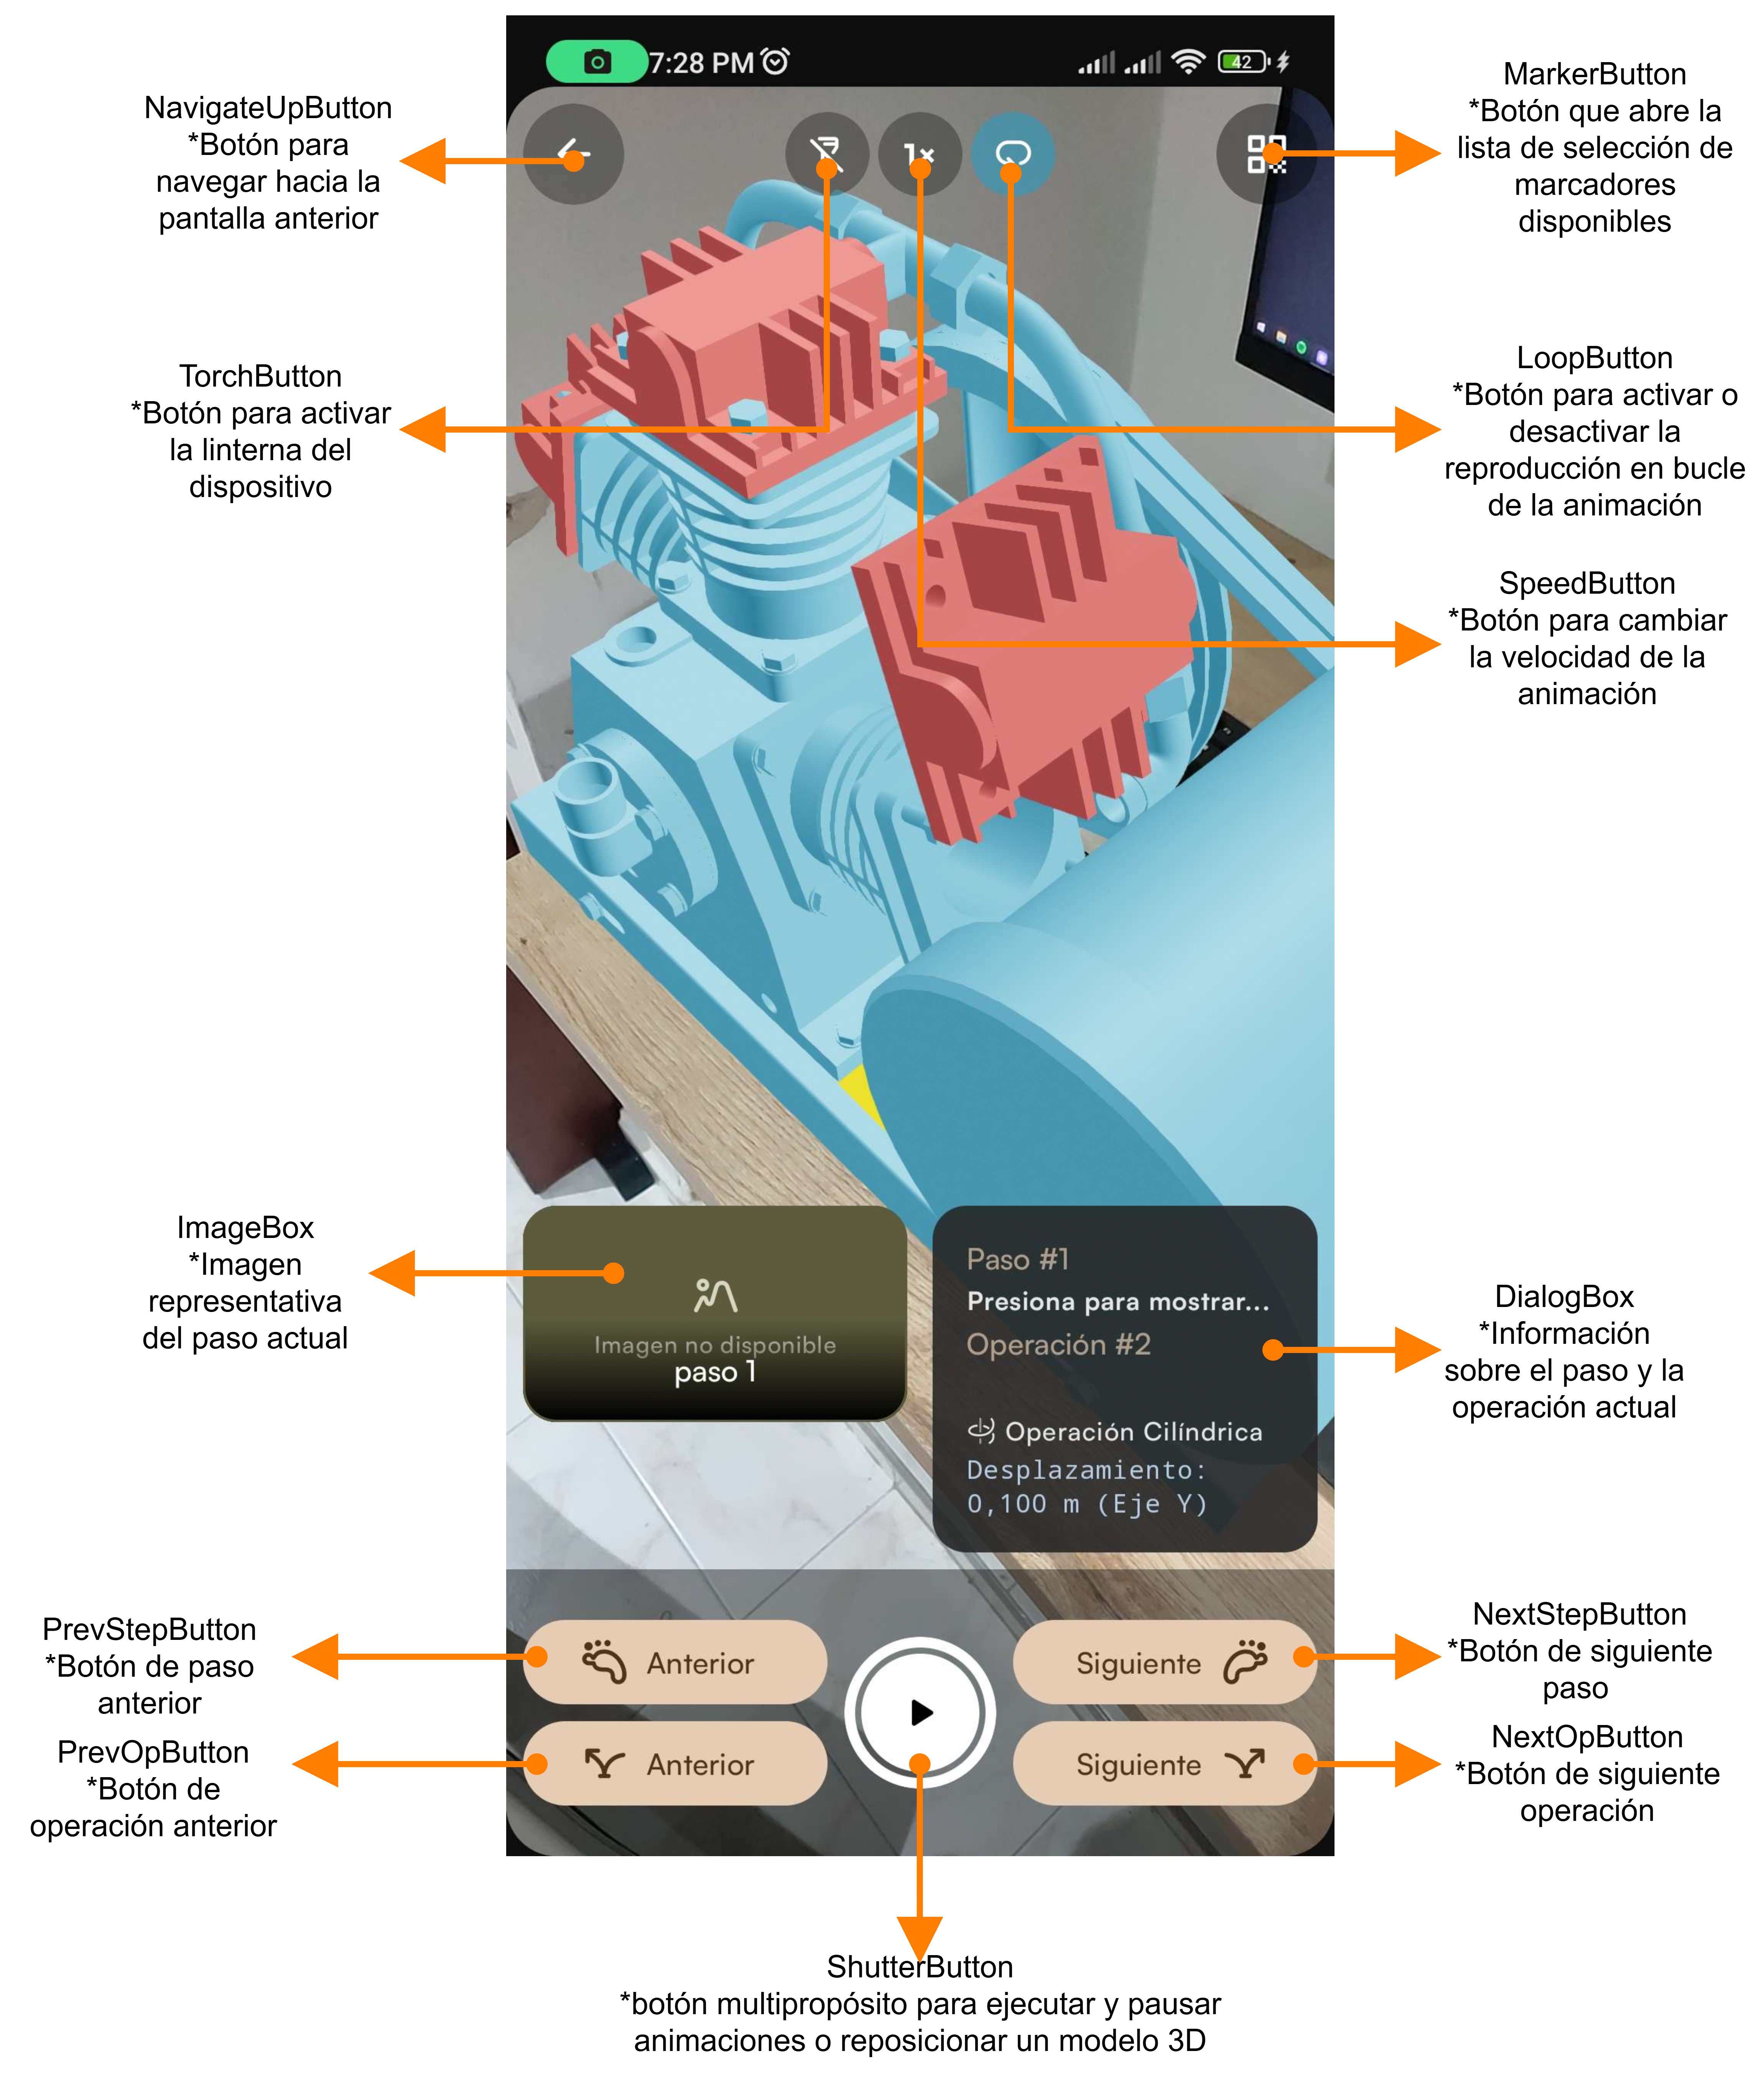
\includegraphics[height=12cm]{assets/figures/second_phase/secondary_screen/img_screen_arsession.png}
    \label{fig:screen_arsession}
\end{figure}

            Como se observa en la Figura \ref{fig:screen_arsession}, la interfaz incorpora una vista de cámara sobre la cual se superponen los modelos tridimensionales y los distintos paneles informativos necesarios para asistir al usuario durante la intervención. Al igual que la pantalla de calibración, implementa un botón de obturador con doble funcionalidad: una pulsación simple reproduce o pausa las animaciones correspondientes a la operación actual, mientras que al mantenerlo presionado se reposicionan los modelos 3D tomando como referencia el marcador activo.

            Los demás controles permiten navegar entre los diferentes pasos de la actividad, mientras que los paneles informativos muestran la descripción e imagen correspondiente a cada uno de ellos. De esta manera, el usuario puede seguir secuencialmente el procedimiento de mantenimiento, visualizando sobre la máquina real las animaciones y la información necesaria para ejecutar cada operación.

    \subsection{Secuencias de los procedimientos de configuración}

        Mediante el lenguaje de modelado visual UML, se elaboraron los diagramas que representan la interacción del usuario con las pantallas que componen la configuración previa con la realidad aumentada. Estos diagramas emplean barras de activación dentro de la línea de vida del usuario, las cuales representan el tiempo requerido para la ejecución de una tarea de forma conceptual.

        \subsubsection{Secuencia para la calibración de modelos 3D}

            La secuencia ilustrada en la Figura \ref{fig:sequence_model_calibration}, muestra el procedimiento que sigue un usuario en la interacción con la pantalla de calibración, donde se insertan modelos 3D que posteriormente se alinearán de forma relativa a un marcador físico por medio del uso de controles de posición y nodos de guías visuales. 

            \begin{figure}[H]
    \caption{Secuencia para la calibración de un modelo 3D}
    \centering
    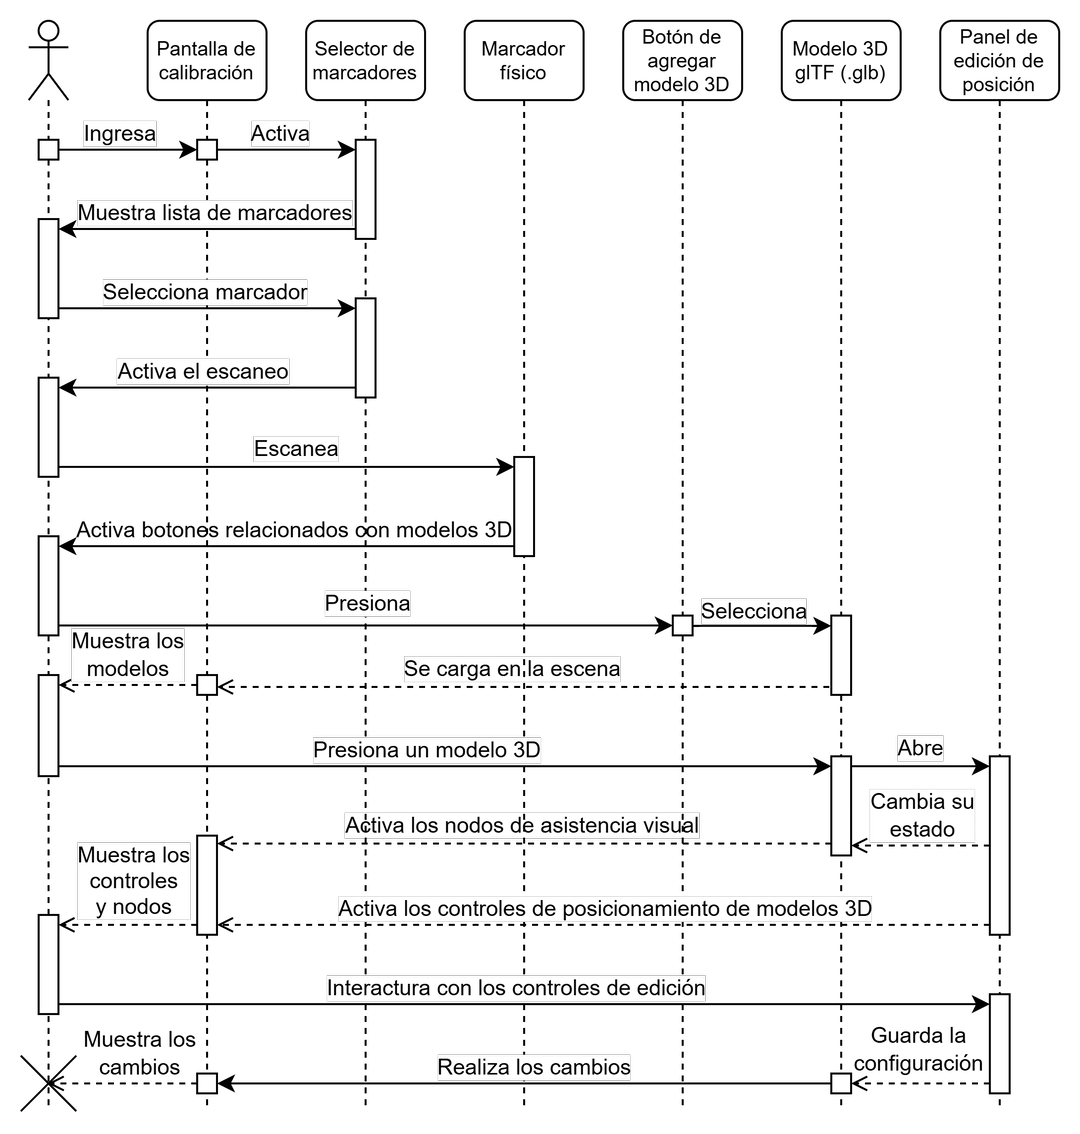
\includegraphics[width=\textwidth]{assets/figures/second_phase/sequence/img_sequence_model_calibration.png}
    \label{fig:sequence_model_calibration}
\end{figure}
\fixvspace{1}

        \subsubsection{Secuencia para la edición de una actividad de mantenimiento}

            La secuencia presentada en la Figura \ref{fig:sequence_activity_edition} describe el procedimiento que sigue el usuario para crear una actividad de mantenimiento y definir los pasos y operaciones que la conforman. Durante este proceso es posible seleccionar los submodelos involucrados y establecer los parámetros necesarios para construir las animaciones que posteriormente serán reproducidas durante la sesión de realidad aumentada.

            \begin{figure}[H]
    \caption{Secuencia para la edición de pasos y operaciones de una actividad}
    \centering
    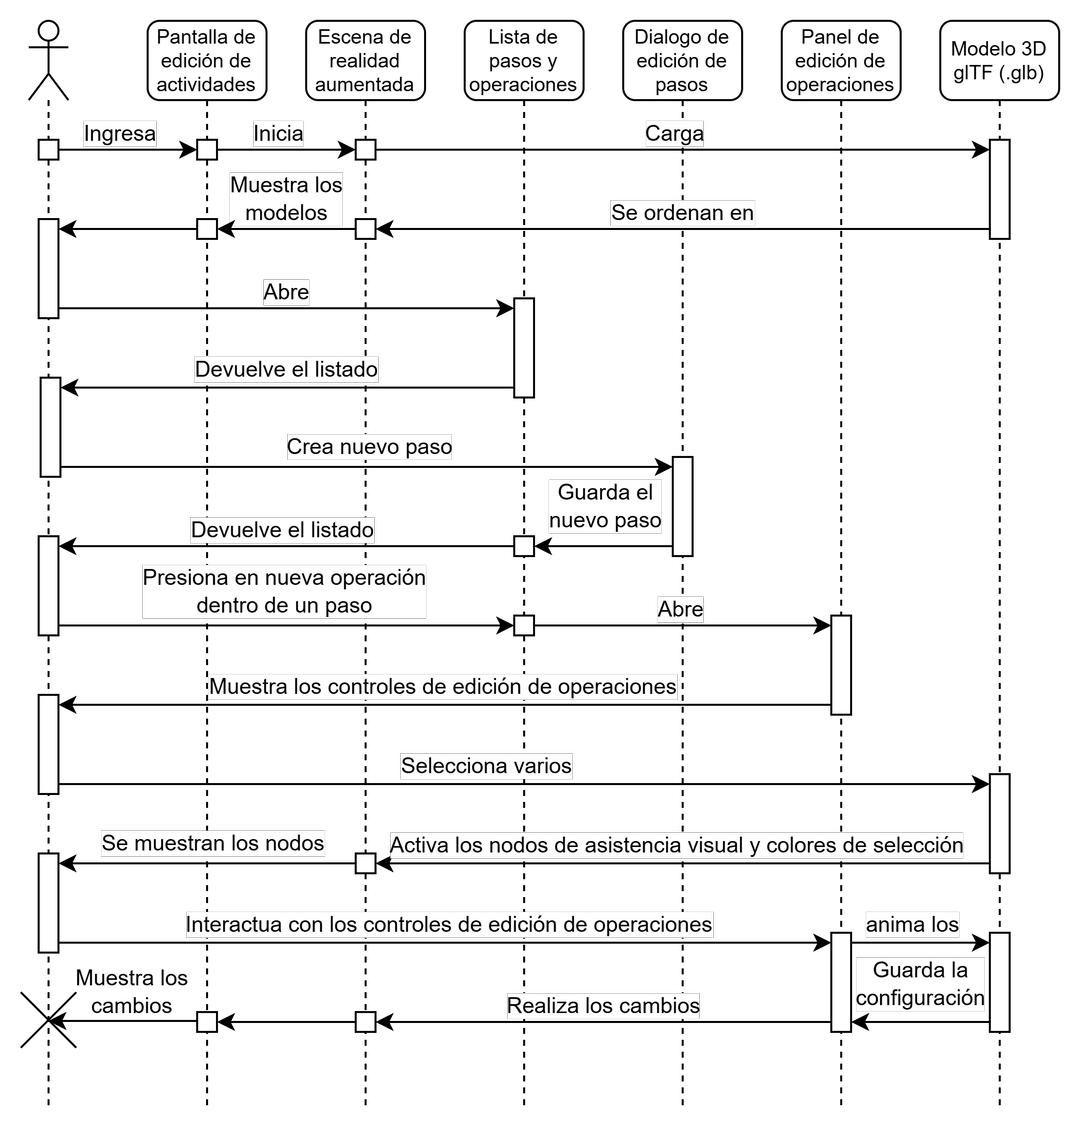
\includegraphics[width=\textwidth]{assets/figures/second_phase/sequence/img_sequence_activity_edition.png}
    \label{fig:sequence_activity_edition}
\end{figure}
\fixvspace{1}